%!TEX root=../paper.tex

\chapter{Architecture and Scheduling Optimization for Active Timing Margin of Voltage Variation}
\label{sec:voltage}

In addition to temperature variation, voltage variation poses unique challenges to active management of processor timing margin. Timing margin must ensure operating reliability under the worst-case, lowest voltage level delivered to transistors, taking into various effects including high loadline, fast $di/dt$ droops, as well as IR drop across the power delivery network (PDN).

In recent years, many hardware techniques have been proposed to  address the high amount of static margin allocated for voltage variation~\cite{kurd2008next,lefurgy2011active,bowman201222nm,grenat20145,tokunaga20145,bowman20158}. These active timing margin solutions schemes aim at reducing the total margin in an agile way to improve system efficiency while still ensuring processor reliability. In this thesis, we present a detailed, full-system characterization of these active timing margin hardware designed specifically for tolerating voltage variation. 

Using measurements and running real-world workloads, we study the factors that affect these active timing margin processors' behavior. Using a fully built production POWER7+ system, we systematically characterize the benefits and limitations of active timing margin in terms of multicore scaling and workload heterogeneity. In our analysis, we cover both active timing margin's undervolting and overclocking modes to fully characterize the system effects under different usage scenarios. 

We find when only one core is active, the current hardware active timing margin schemes can efficiently turn the underutilized timing margin into significant power and performance benefits while tolerating voltage swings. However, as more cores are progressively utilized by a multithreaded application, the benefits of active margin begin to diminish in both power and performance improvements. Using POWER7+'s sensor-rich features, we systematically characterize and decompose the on-chip voltage drop that affects the active timing margin's efficiency into its different components, and analyze the root cause of the problem. Under heavy load, the IR drop across the chip and the voltage regulator module's (VRM) loadline effect limit active timing margin's ability to the point of almost no benefit. 

The magnitude of the efficiency drop aforementioned, however, varies significantly from one workload to another. Thus, given the workload sensitivity of hardware active timing margin techniques, and the long-term nature of the observed effects, we introduce the notion of \emph{adaptive margin scheduling (AMS)}. The intent behind AMS is to compensate for active margin's inefficiencies in system software. The remainder of this section is structured as follows: \Sec{sec:voltage:background} provides background for the POWER7+ architecture and its implementation of active timing margin for voltage variation. \Sec{sec:voltage:characterization} characterizes active margin's limitations when scaling up the number of active cores under different workload scenarios. \Sec{sec:voltage:rootcause} analyzes the root cause of active margin's behavior as seen in the previous section. \Sec{sec:voltage:opt} proposes active timing margining scheduling to improve POWER7+'s efficiency when the load is light versus heavy. \Sec{sec:voltage:related} compares our work with prior work.

\section{Active Timing Margin in the POWER7+ Multicore Processor}
\label{sec:voltage:background}

\TODO{to be merged with the next chapter}

The POWER7+ is an eight-core out-of-order processor manufactured on a 32-nm process. It supports 4-way simultaneous multithreading, allowing a total of 32 threads to execute simultaneously on the system~\cite{manousopoulos2012characterizing}.

A POWER7+ processor has two main power domains, each with its own on-chip power delivery network (PDN). The V$_{dd}$ domain is dedicated to the logic circuits in the core and caches, and the V$_{cs}$ domain is dedicated for the on-chip storage structures~\cite{zyuban2013ibm,barth201045nm}. The PDNs are shared among all eight cores to reduce voltage noise~\cite{james2007comparison}. In our study, we primarily focus on voltage variation over the logic circuits's power domain as it is the main power consumer.

The processor supports both coarse-grained and fine-grained power management. Coarse-grained power management includes per-core power gating to reduce idle power consumption. Fine-grained power management is the active timing margin. In our later AMS optimization, we combine these two schemes to enhance the processor's overall efficiency.

POWER7+ uses active timing to prevent circuit timing emergencies~\cite{lefurgy2011active,lefurgy2013active,floyd2013runtime}. Although the implementation of active timing margin for voltage variation can vary from one platform to another~\cite{fischer200590nm,tschanz2007adaptive,kurd2008next,lefurgy2011active,bowman201222nm,grenat20145,tokunaga20145,bowman20158}, the general building blocks and principles largely remain the same. 
In POWER7+, clock cycle time is variable and actively tracks circuit speed from cycle to cycle. In the event of a voltage droop, the processor slows down the cycle time to allow circuit operation to complete. Because voltage droops occur rarely, during normal operation the active timing margin mechanism eliminates a significant portion of the timing slack.

\begin{figure*}[t]
\centering
\subfloat[Control loop overview.] {
   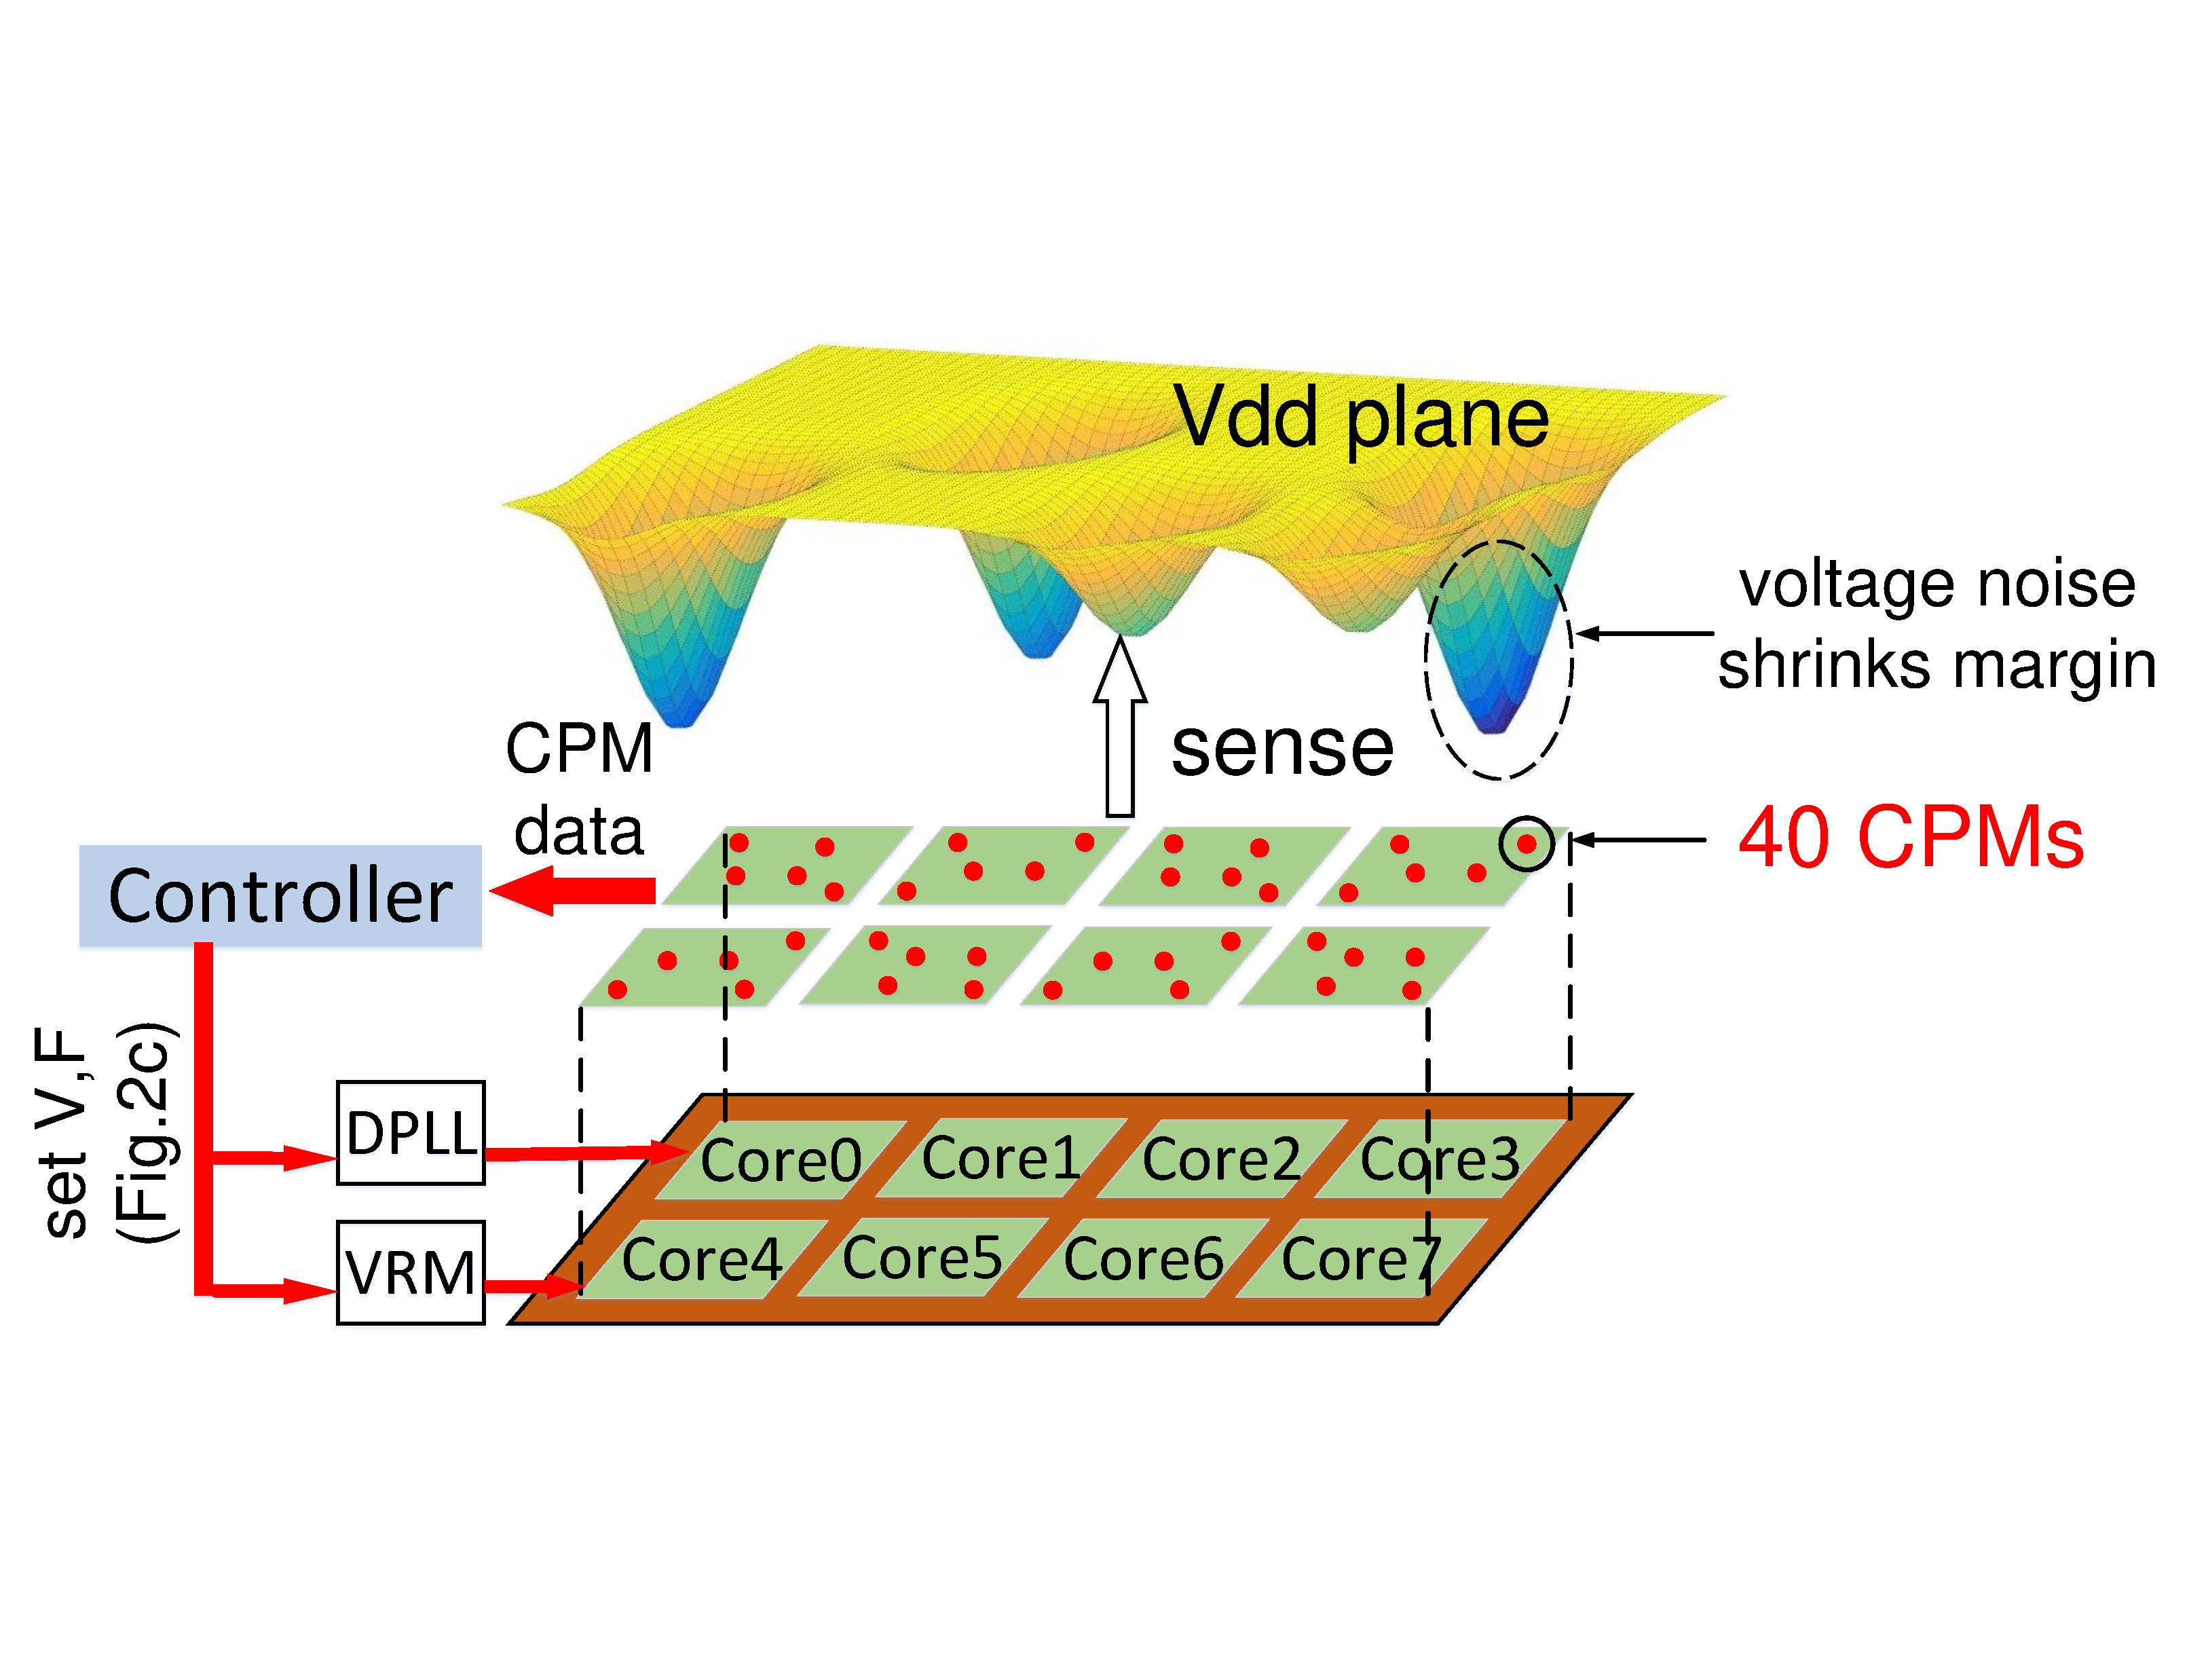
\includegraphics[trim=0 250 0 260,clip,width=.625\linewidth]{graphs/voltage/control-loop.pdf}
   \label{fig:control-loop} 
}
\subfloat[CPM behavior.] {
   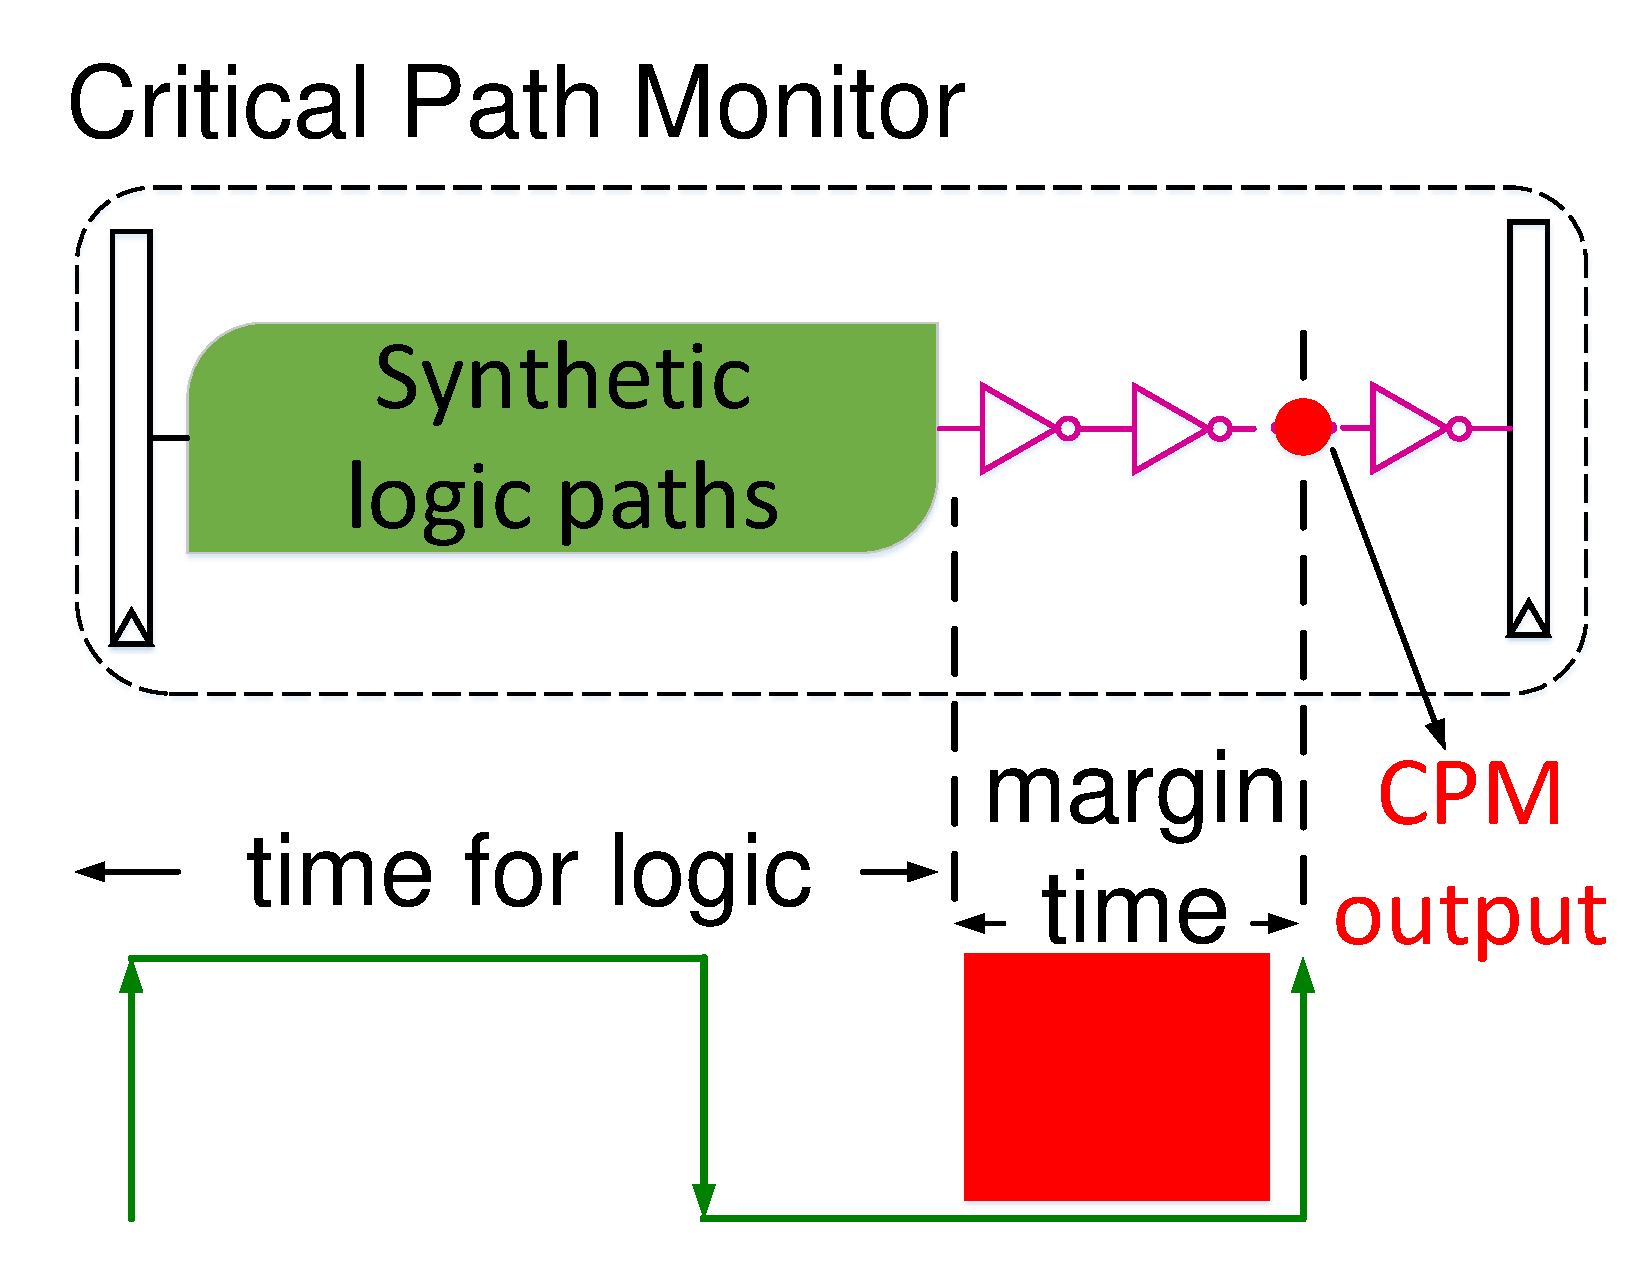
\includegraphics[trim=0 20 0 20,clip,width=.385\linewidth]{graphs/voltage/CPM-structure.pdf}
   \label{fig:cpm_internal} 
}
\caption{Interactions among CPMs, DPLLs, and VRMs to guarantee reliability and improve efficiency in POWER7+. CPM measures the timing margin and the controller adjusts voltage and frequency accordingly.}
\end{figure*}

\Fig{fig:control-loop} shows an overview of the feedback loop for active timing margin control. The system relies on three key components: (1) critical path monitor (CPM) sensors to sense timing margin~\cite{drake2007distributed,drake2013single}; (2) digital phase locked loops (DPLLs) to quickly and independently adjust clock frequency per core based on CPM readings~\cite{tierno2010dpll}; and (3) hardware and firmware controllers that decide when and how to leverage the benefits from a tighter timing margin.

POWER7+ has 40 CPMs distributed across the chip to provide chip-wide, cycle-by-cycle timing margin measurement. Each core has 5 CPMs placed in different units to account for core-level spatial variations in voltage noise and critical path sensitivity. Detailed characterization of CPM placement, calibration, and sensitivity is provided in~\cite{floyd2013runtime}.

A CPM uses synthetic paths to mimic different logical circuits' behavior and a 12-bit edge detector to quantify the amount of timing margin left. \Fig{fig:cpm_internal} illustrates the CPM's internal structure. On each cycle, a signal is launched through the synthetic paths and into the edge detector. When the next cycle arrives, the number of delay elements the edge has propagated through in the edge detector corresponds to the CPM output. A CPM outputs an integer index from 0--11, which corresponds to the position of the edge in the edge detector.

In the POWER7+ processor, during chip testing the different CPMs are calibrated to output a target value.  When the output is less (toward zero), the timing margin has been reduced from the calibrated point. Likewise, when the output is more (toward 11), the available timing margin has increased.

Per-core DPLL frequency control lets the processor tolerate transient voltage droops by reducing clock frequency for each core with no impact on other cores. The DPLLs can rapidly adjust frequency, as fast as 7\% in less than 10 ns, while the clock is still active; thus, the processor can tolerate transient voltage droops. Every cycle, the lowest-value CPM in each core is compared against the calibration position. In response, the DPLL will slew the clock frequency up or down to control the timing margin to the calibrated amount. 

POWER7+ supports two modes to convert the excess timing margin into either a performance increase by overclocking or power reduction by undervolting. In the overclocking mode, the CPM and DPLL hardware form a closed-loop controller. At the fixed nominal voltage, the DPLL continuously adjusts frequency on the basis of the CPM's timing sense to operate at the calibrated timing margin. Under light loads, clock frequency can be boosted by as much as 10\% compared to when active timing margining is off. In the undervolting mode, the firmware observes CPM-DPLL's frequency and over a longer term (32ms) adjusts voltage to make clock frequency hits the target. In this case, the performance benefit from the CPM-DPLL can be turned into an energy-saving benefit.

\section{Efficiency Analysis of Active Timing Margin on Multicore}
\label{sec:voltage:characterization}

Most prior art studied the benefits of mitigating voltage variation and reducing timing margin at the circuit-~\cite{kurd2008next,bowman201222nm,grenat20145,tokunaga20145,bowman20158} and architecture levels~\cite{lefurgy2011active,reddi2009voltage,gupta2008decor,powell2003pipeline,reddi2010voltage,bertran2014voltage} using homogeneous single-core workloads. This thesis focuses on understanding the efficiency of active timing margin on a multicore system, specifically as the system activity (i.e., core usage) begins to increase using real workloads.

Using an enterprise class server (\Sec{sec:voltage:characterization:setup}), we characterize the efficiency of active timing margin at the system level. In particular, we measure, analyze and characterize active timing margin's effectiveness under different architectural configurations and workload characteristics. We make two fundamentally new observations about the effectiveness of active timing margin on a multicore system. First, the efficiency of active timing margin can diminish as the number of active cores increases (\Sec{sec:voltage:characterization:scaling-trends}). Second, the inefficiency is highly subject to workload characteristics (\Sec{sec:voltage:characterization:workload-variation}).

\subsection{Experimental Infrastructure}
\label{sec:voltage:characterization:setup}
 
We perform our analysis on a commercial IBM Power 720 Express server (7R2) that has two POWER7+ processors on the motherboard. The processors share the main memory and other peripheral resources, such as storage and network. We focus on one of the two processors, although we validated our conclusions by conducting experiments on the other processor as well. Unless stated otherwise, the first processor is configured to idle and runs background tasks. The system runs RedHat Enterprise Linux, configured with 32~GB RAM. 

We use PARSEC~\cite{bienia2008parsec} and SPLASH-2~\cite{woo1995splash,bienia2008parsecsplash} in this section because they are scalable workloads and we need to the control the applications' parallelism to carefully study the impact of core scaling. The workloads are compiled using GCC with \texttt{-O2} optimization.

We characterize the efficiency of active timing margin across two modes of operation: 1) undervolting to reduce power consumption and 2) overclocking to boost performance. Hooks in the firmware let us place the system in either operating mode. The hardware and firmware autonomously select frequency and voltage depending on the configured operation mode.

\subsection{Core Scaling}
\label{sec:voltage:characterization:scaling-trends}
Using \benchmark{raytrace} from PARSEC (as an example), we show active timing margin's impact on chip power. We study both average chip power consumption and total CPU energy savings using \Fig{fig:raytrace-inefficiency}. We find that active timing margin is always effective at improving performance or lowering power consumption. However, it cannot always scale up efficiently with more cores. 

\begin{figure}[t]
	\centering
    \subfloat[Power saving.] {
      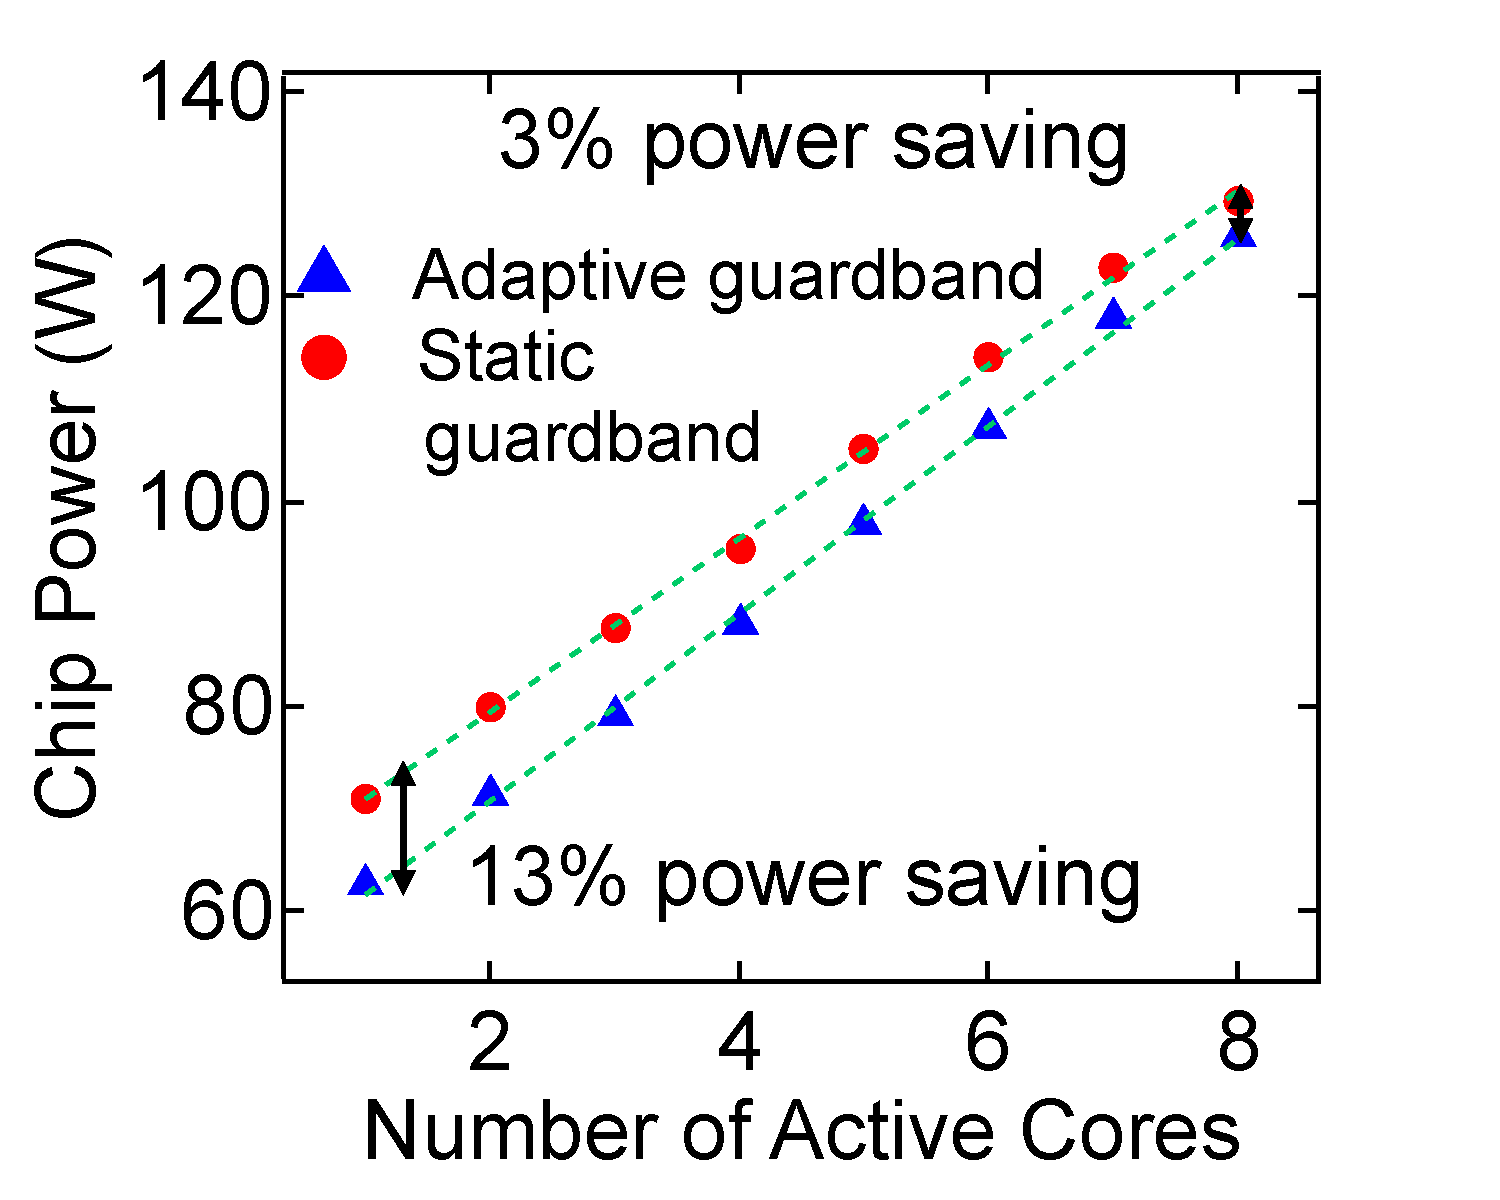
\includegraphics[trim=0 0 0 0,clip,width=.4\linewidth]{graphs/voltage/raytrace_pwr.pdf}
      \label{fig:raytrace-ineff_pwr} 
    }
    \subfloat[Energy reduction.] {
       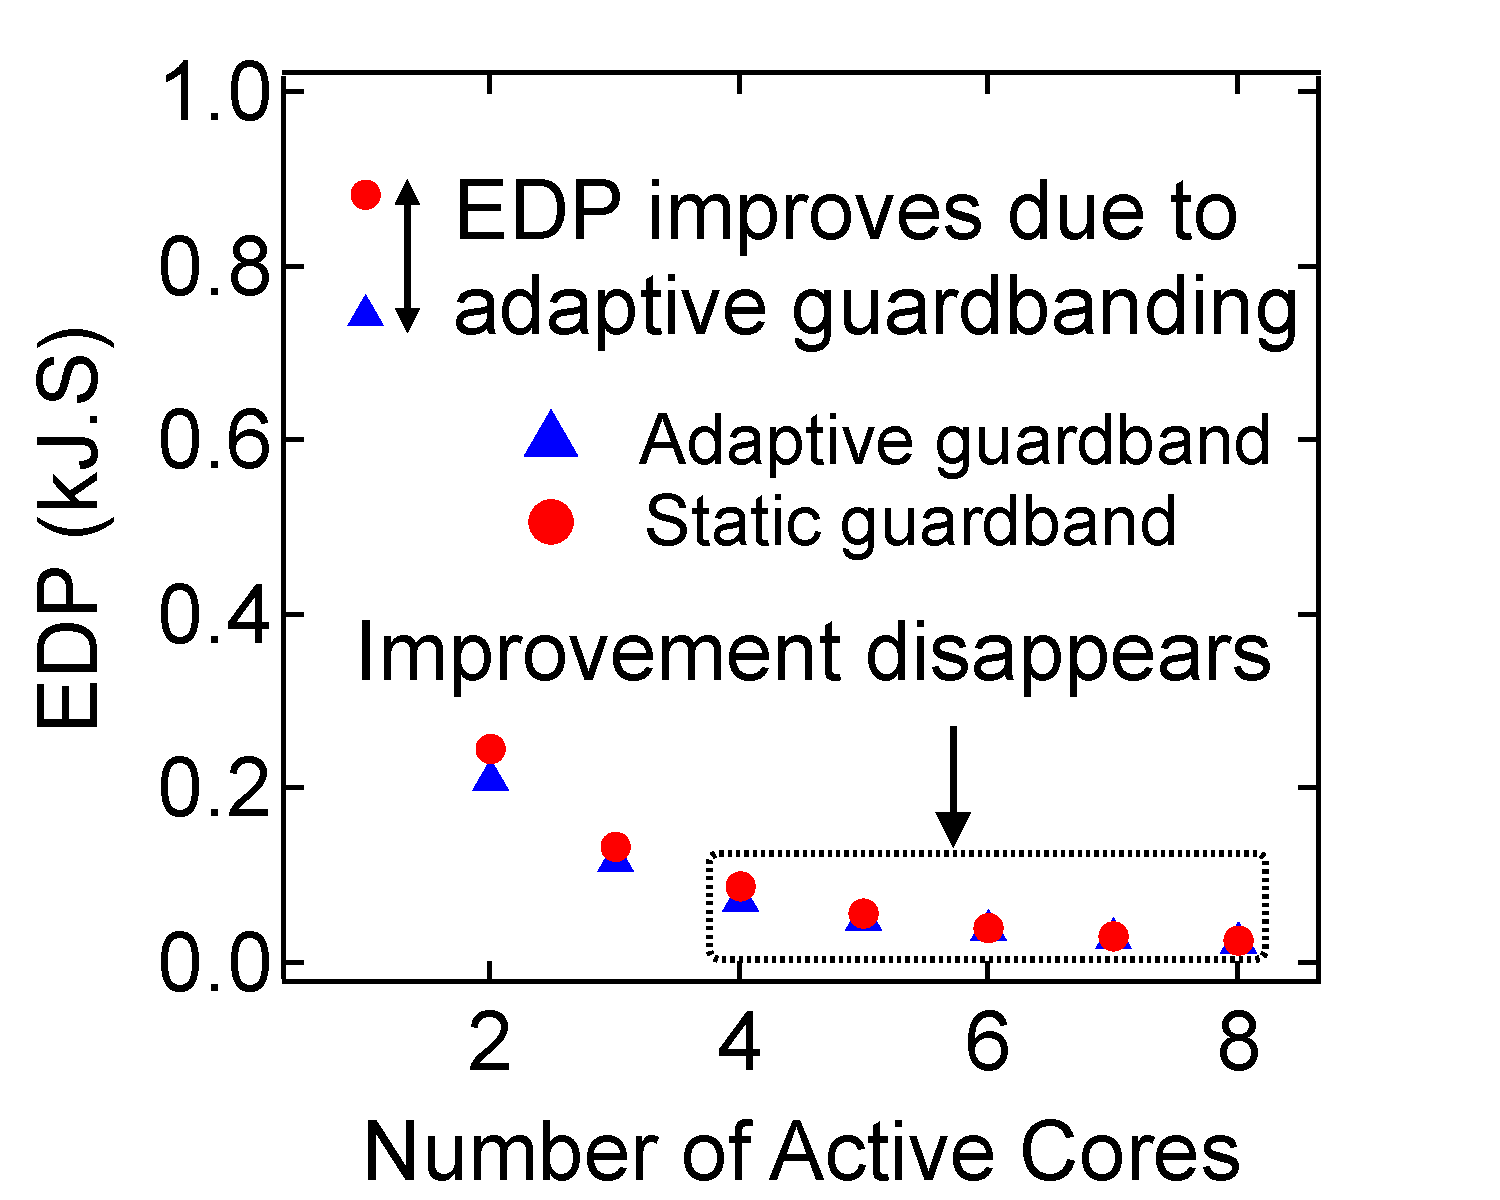
\includegraphics[trim=0 0 0 0,clip,width=.4\linewidth]{graphs/voltage/raytrace_edp.pdf}
       \label{fig:raytrace-ineff_edp} 
    }
    \caption{Active timing margin can save power effectively. However, the benefits decrease as more cores are used to actively run the application.}
    \label{fig:raytrace-inefficiency}
\end{figure}

\Fig{fig:raytrace-ineff_pwr} shows the program's power consumption as we use more cores, i.e., more threads to process the workload. We measure the microprocessor V$_{dd}$ rail power by reading physical sensors available on the server, which represents most of the total processor power. In undervolting mode, active timing margin turns the unused margin into energy savings by scaling back the voltage, which reduces unnecessary power consumption. When one core is active and the others are idle, active timing margin reduces the average power consumption by 13\% compared to no active timing margining. 

Although active timing margin always saves power, a more important and crucial observation from \Fig{fig:raytrace-ineff_pwr} is the decreasing power-saving trend as the number of active cores increases in the system. The power improvement from active timing margin decreases as the parallelism in the workload is (manually) increased, forcing the usage of the additional cores. Although active timing margin can save as much as 13\% power when only one core is active, the savings drop sharply to about 3\% when the activity scales up to eight cores.

When examining the workload's overall energy-delay product (EDP), \Fig{fig:raytrace-ineff_edp} shows notable energy efficiency improvement when only a small set of cores is actively processing the workload. However, beyond four cores, the improvement drops significantly. When only one core is active, processor energy efficiency improves by as much as 20\% compared to using a static margin. But the additional improvement beyond activating more than four cores becomes negligible. 

Our observations hold true for frequency-boosting as well. Active timing margin's ability to boost frequency decreases as core counts increase. \Fig{fig:lucb-inefficiency} shows experimental results for \benchmark{lu\_cb} from the SPLASH-2 benchmark suite. Compared to using a fixed target frequency of 4.2GHz under a static margin, active timing margin can achieve substantial frequency improvement, as shown in~\Fig{fig:lucb-ineff_freq}. When only one core is actively processing the workload, frequency increases by up to 10\% compared to the static margin baseline. However, when all eight cores are running the workload the frequency gain drops to only 4\%.

\begin{figure}
%\vspace*{-.15in}
\centering
    \subfloat[Frequency-boosting mode.] {
        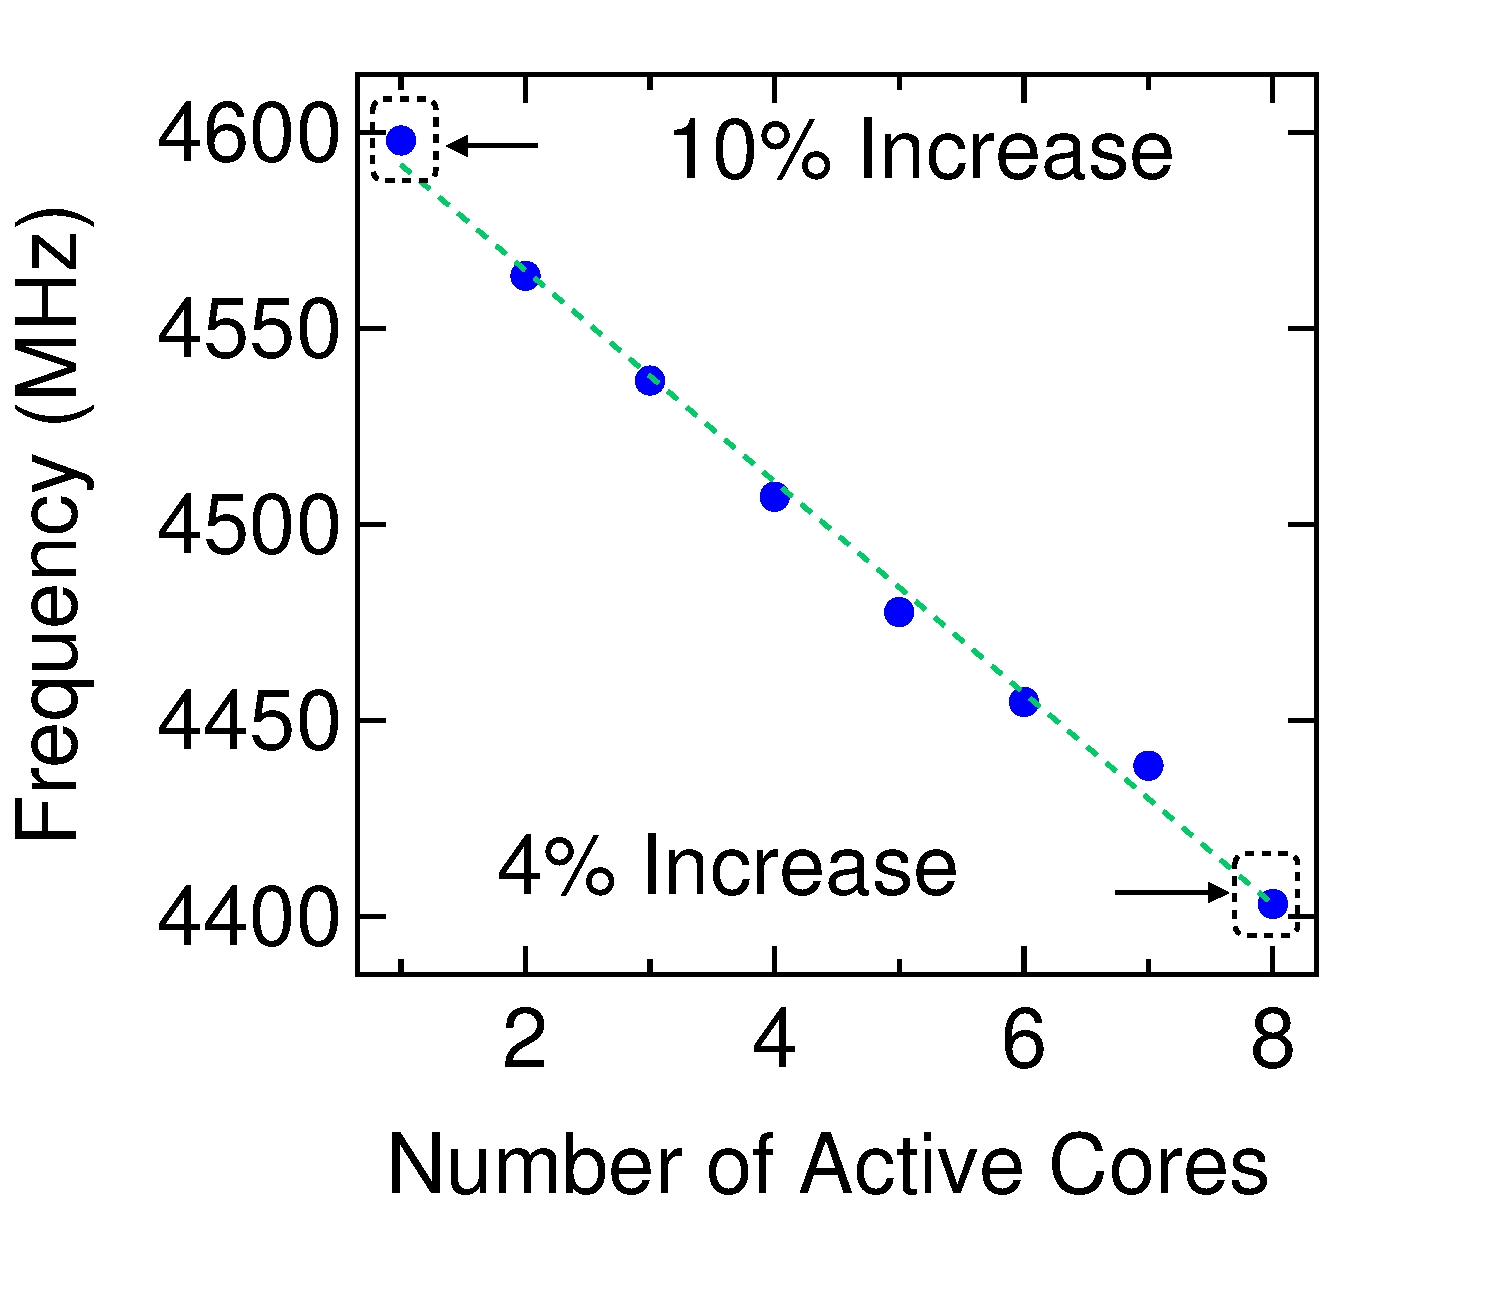
\includegraphics[trim=0 45 65 35,clip,width=.38\linewidth]{graphs/voltage/lucb_freq.pdf}
        \label{fig:lucb-ineff_freq} 
      }
    \subfloat[Execution time.] {
        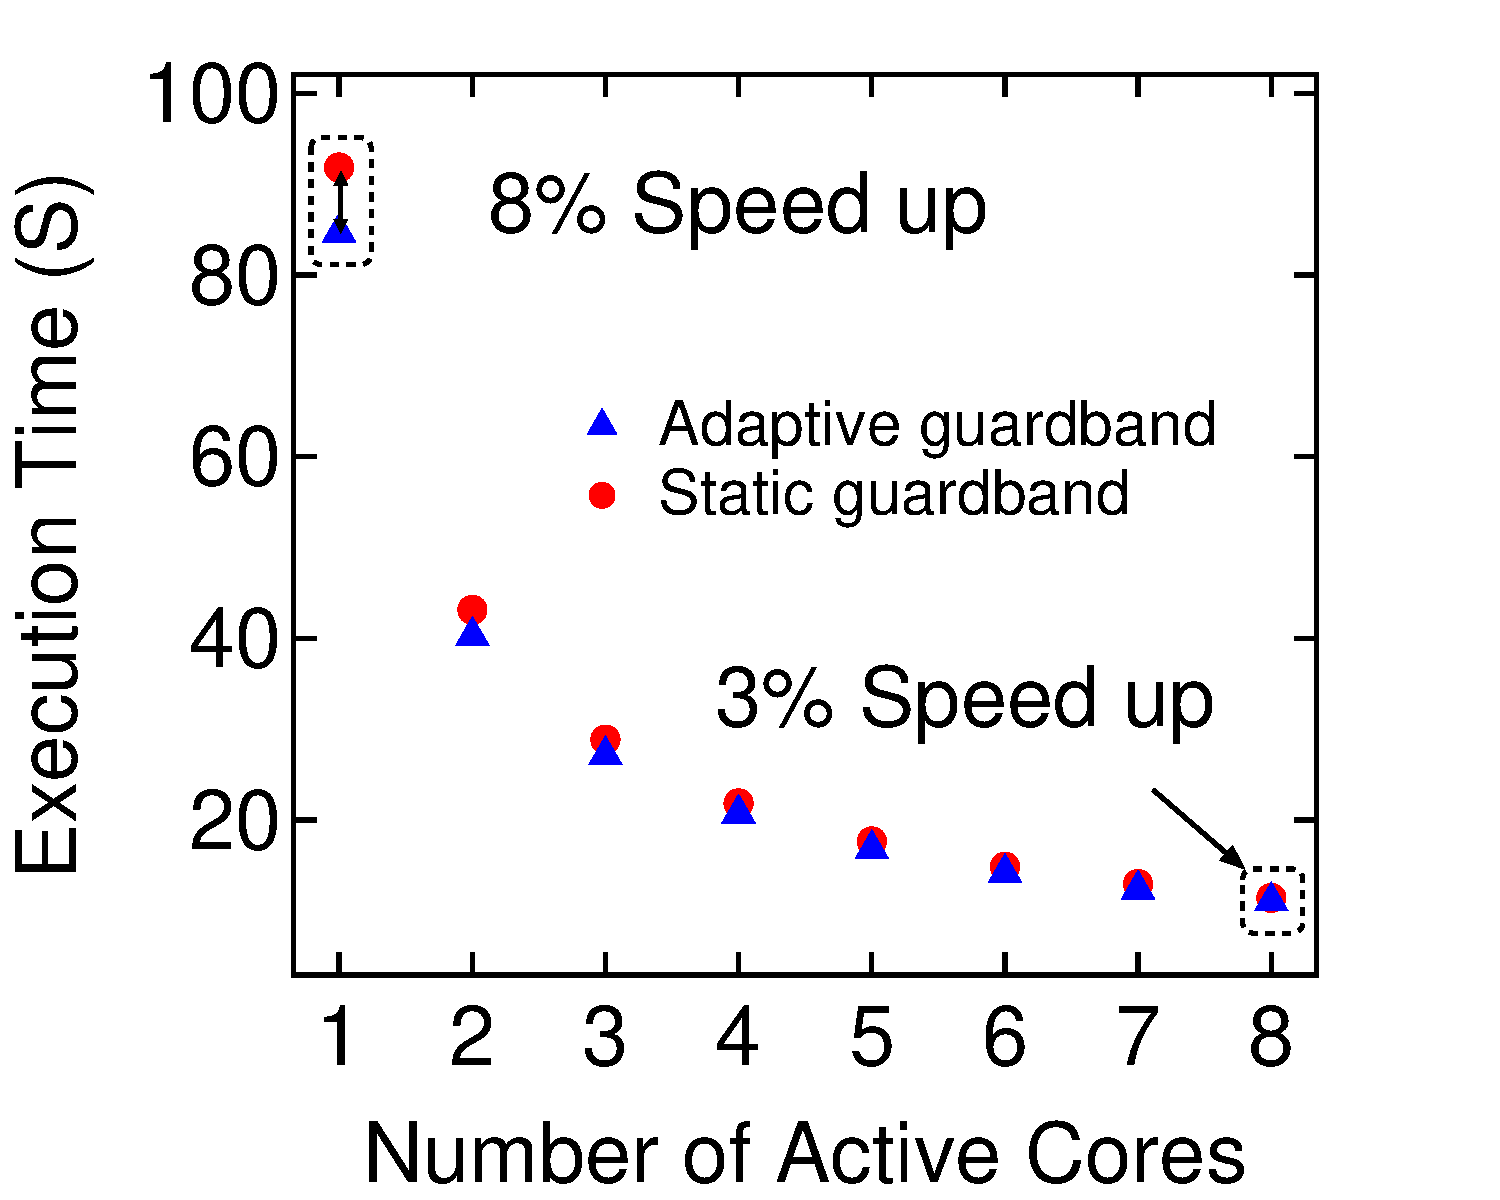
\includegraphics[trim=0 0 65 0,clip,width=.38\linewidth]{graphs/voltage/lucb_time.pdf}
        \label{fig:lucb-ineff_speedup} 
      }
    \caption{Active timing margin can improve performance by increasing frequency. However, the overclocking benefits decrease as more cores are used.}
    \label{fig:lucb-inefficiency}
 \end{figure}

Frequency improvement turns into program execution time speedup, especially for computing-bound workloads. For \benchmark{lu\_cb} the execution speedup varies gradually, decreasing from 8\% when only one core is used to 3\% when all cores are running the workload. This trend of diminishing benefit as core count scales up is similar to what we observe when the extra guardband is turned into energy savings for this workload. 

\subsection{Workload Heterogeneity}
\label{sec:voltage:characterization:workload-variation}

Variations in workload activity (i.e., heterogeneity) are known to strongly impact system performance from cache performance to bandwidth utilization. In this section, we demonstrate workload heterogeneity also impacts active timing margining's runtime efficiency. We focus our analysis on the architecture-level observations and later in \Sec{sec:voltage:rootcause} we explore the causes for the observed behaviors.

\Fig{fig:workloadvariation} shows the results for power and frequency improvement for all PARSEC and SPLASH-2 workloads compared to the same number of cores active when active timing margin is disabled. The improvements are with respect to the system using a static guardband. The results are from two experiments, one in which the control loop is operating in energy-saving mode (\Fig{fig:pwrvariation}) and the other in which it is operating in frequency-boosting mode (\Fig{fig:freqvariation}). Each line in both figures corresponds to one benchmark.

From \Fig{fig:pwrvariation} and \Fig{fig:freqvariation}, we draw four conclusions. First, active timing margining consistently yields improvement, regardless of its operating mode and workload diversity. Across all of the workloads, active timing margining reduces power consumption somewhere between 10.7\% and 14.8\% and improves processor clock frequency by as much 9.6\% on average, when one core is active. Even when all eight cores are active, improvements are at least above 4\%. Power-saving improvements are slightly larger than frequency improvements because of the quadratic relationship between voltage scaling and power, as opposed to the linear relationship between frequency and power.

\begin{figure}[t]
\vspace*{-.15in}
\centering
  \subfloat[Power-saving mode.] {
    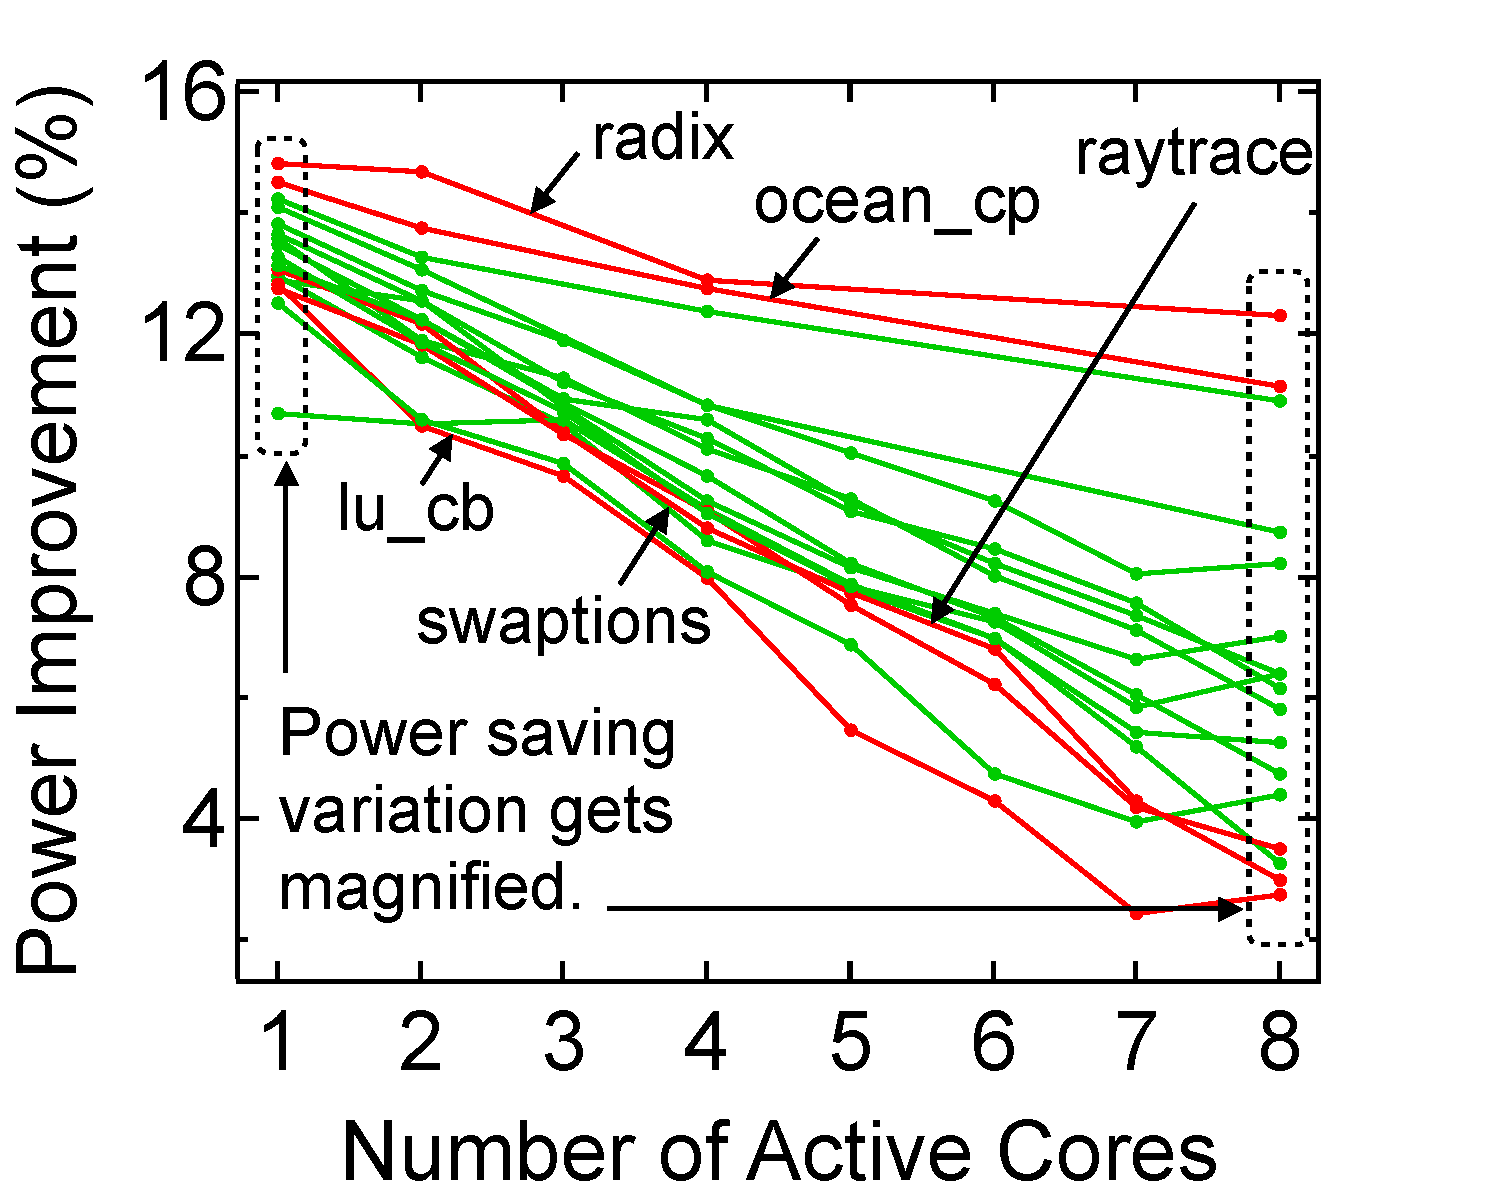
\includegraphics[trim=0 0 0 0,clip,width=.45\linewidth]{graphs/voltage/power_saving_variation.pdf}
    \label{fig:pwrvariation} 
  }
  \subfloat[Frequency-boosting mode.] {
    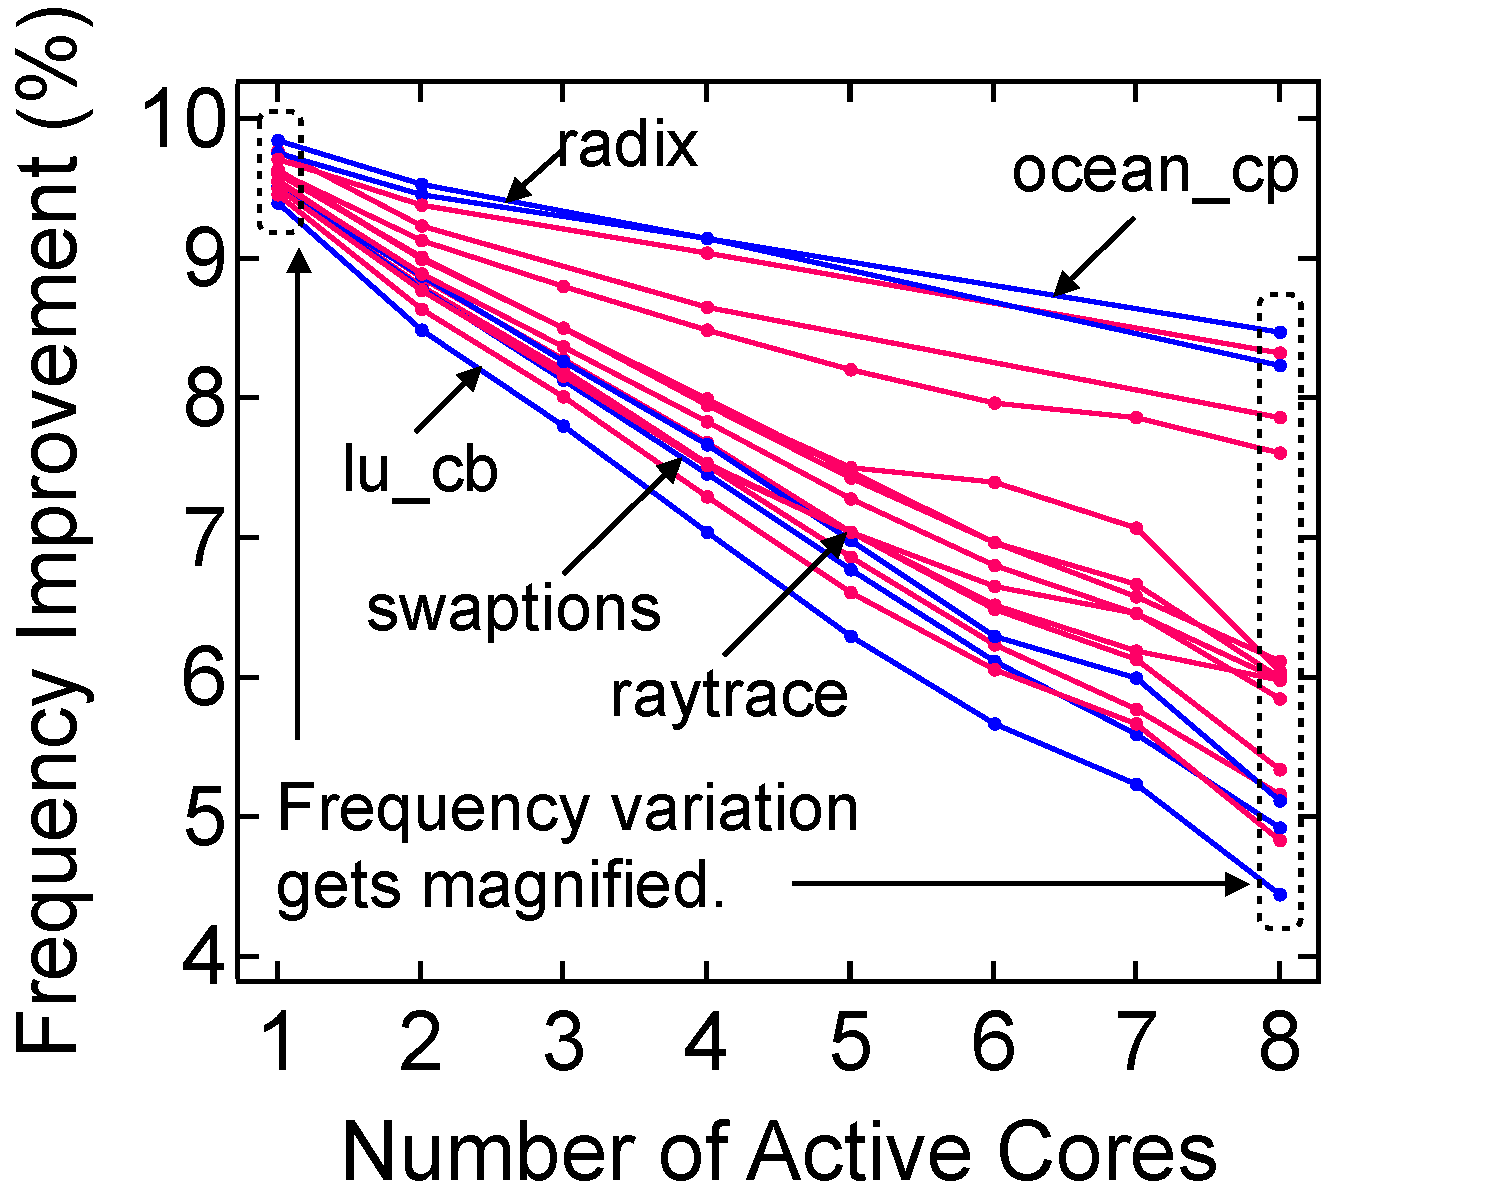
\includegraphics[trim=0 0 0 0,clip,width=.45\linewidth]{graphs/voltage/freq_saving_variation.pdf}
    \label{fig:freqvariation} 
  }
  \caption{Improvements reduce at different rates for each of the PARSEC and SPLASH-2 workloads when cores are progressively activated, leading to magnified workload variation when all cores are active.}
\label{fig:workloadvariation} 
\vspace{-0.2cm}
\end{figure}

Second, the improvements monotonically decrease as the number of active cores increases. Across all the workloads, we observe a consistent drop in active timing margining's efficiency. The average power efficiency improvement across the workloads drops from 13.3\% when one core is active to 10\% when two cores are active to 6.4\% when all cores are actively processing the workload. We observe a similar trend with frequency.

Third, the rate of monotonic decrease for each workload varies significantly. For instance, \benchmark{radix}'s power improvement drops from 15\% when one core is active to around 12\% when all eight cores are active. However, in \benchmark{swaptions}, the improvement drops drastically from 13\% to 3\%. In the frequency-boosting mode, the decreasing magnitude is slightly smaller, although the variation in improvements is still strongly present. Frequency for \benchmark{radix} and \benchmark{ocean\_cp} almost remains unchanged at 9\%, but the frequency of \benchmark{lu\_cb}, \benchmark{swaptions} and \benchmark{raytrace} drops notably from 10\% to 4\%.

Fourth, regardless of the active timing margining operating mode (i.e., power saving or frequency boosting), workload heterogeneity significantly impacts the mechanism's efficiency when all cores are active. This finding is especially important in the context of enterprise systems, because server workloads are ideally configured to fully use all computing resources to reduce the operator's total cost of ownership (TCO)~\cite{barroso2007case}. 

In multicore systems that rely on active timing margining, the system's behavior will vary significantly depending on how many cores are being used and what workloads are simultaneously coscheduled for execution on the processor. To prove this point, we later discuss the implications of workload coscheduling using our system. In the future, we suspect workload heterogeneity could be a major source of inefficiency, especially as we integrate more cores into the processor, unless we identify the problem's source for mitigation.

\section{Root-Cause Analysis of Active Timing Margin's Inefficiencies}
\label{sec:voltage:rootcause}

In this section, we analyze the root cause of active timing margin's inefficiency under increasing core counts and workload heterogeneity to understand how to reclaim the loss in efficiency. We present an approach for characterizing active timing margin's inefficiency using CPM sensors (\Sec{sec:voltage:rootcause:cpm-measurement}). On this basis, we characterize the voltage drop in the chip across both core counts and workloads because the on-chip voltage drop affects active timing margin's efficiency. Our analysis reveals that core count scaling results in a large on-chip voltage drop (\Sec{sec:voltage:rootcause:vdrop-analysis}), whereas workload heterogeneity plays a dominant role in affecting the processor's IR drop and loadline (\Sec{sec:voltage:rootcause:vdrop-decompose}).

\subsection{Measuring the On-chip Voltage Drop}
\label{sec:voltage:rootcause:cpm-measurement}

\begin{figure*}[t]
\centering
  \subfloat[Mapping between on-chip voltage and CPM values.] {
      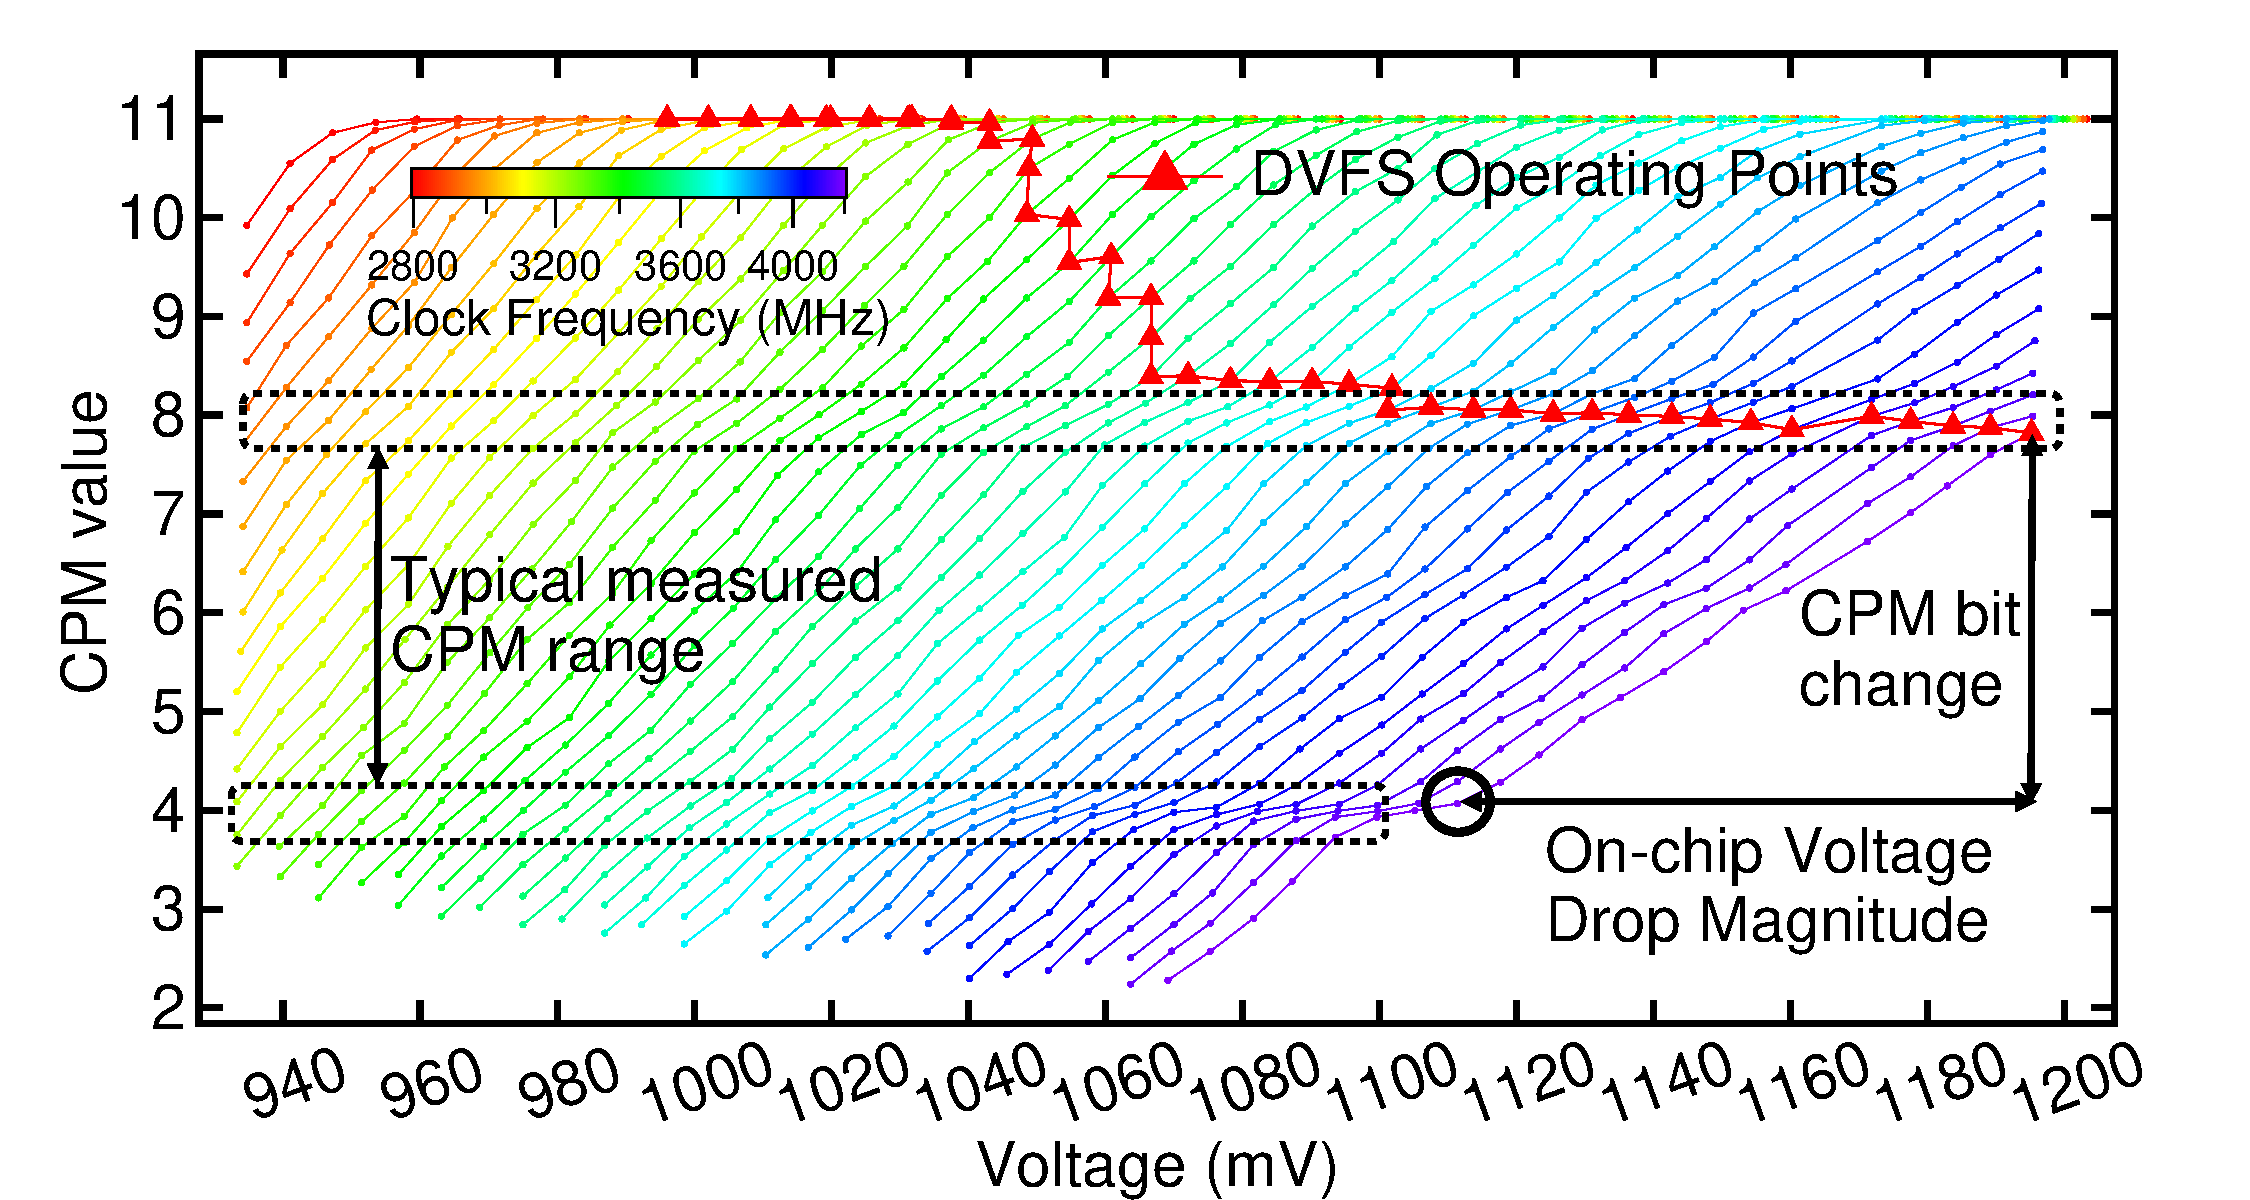
\includegraphics[trim=25 0 25 0,clip,width=0.425\linewidth]{graphs/voltage/cpm2volt.pdf}
      \label{fig:cpm2volt} 
  }
  \subfloat[The CPMs' sensitivity toward supply voltage in each core.] {
      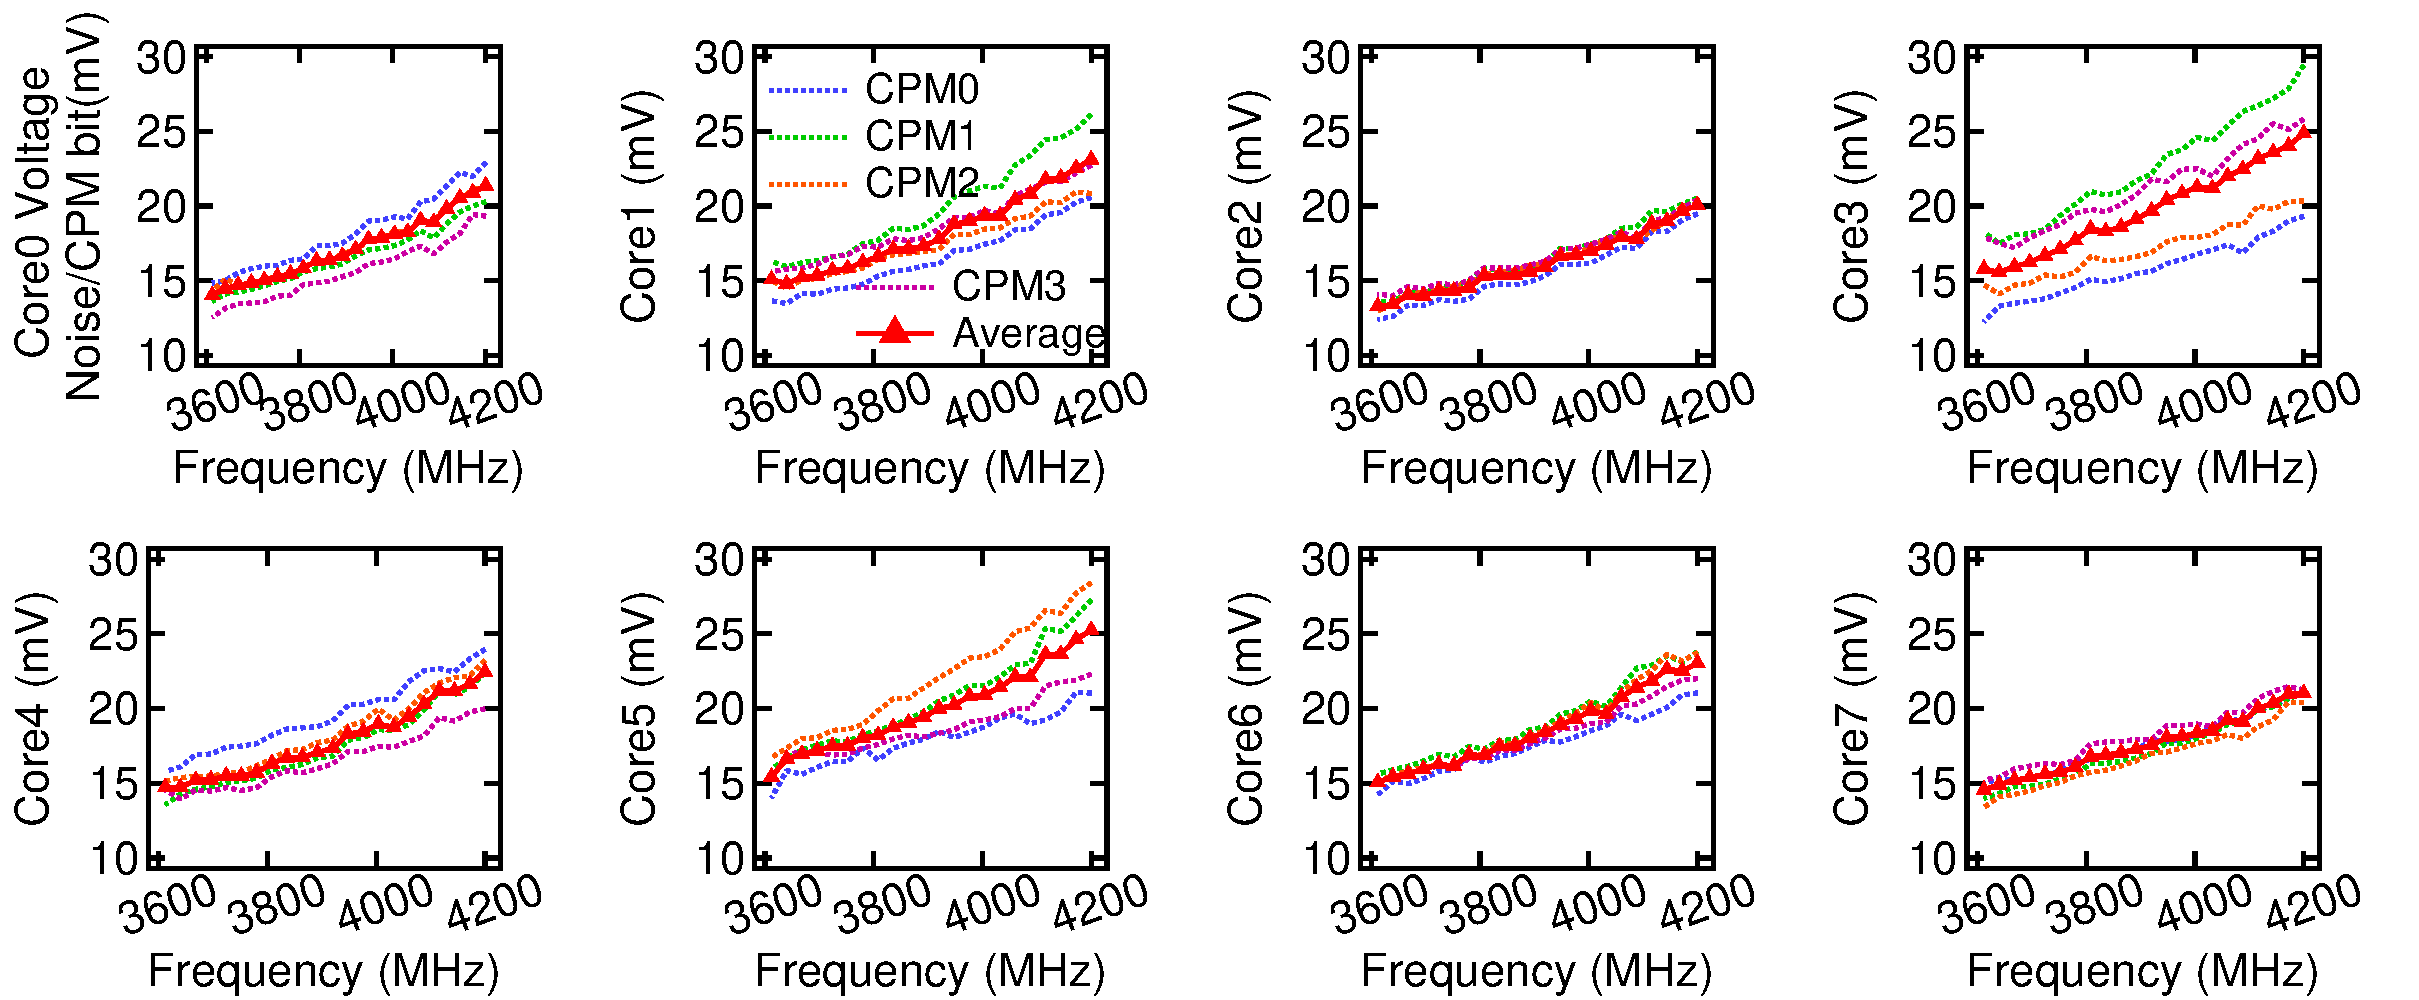
\includegraphics[trim=5 0 10 0,clip,width=0.575\linewidth]{graphs/voltage/cpm_process_variation.pdf}
      \label{fig:cpmsensitivity} 
  }
\caption{CPMs can sense the chip supply voltage with a precision of about 21mV per CPM bit at peak frequency.}
\label{fig:cpm-analysis}
\end{figure*}

We developed a novel approach to capture and characterize active timing margin's behavior using CPMs. We use CPM output to capture the on-chip voltage drop that affects the timing margin, which in turn affects the active timing margin's efficiency. In effect, we use CPMs as ``performance counters'' to estimate on-chip voltage, similar to how performance counters were first shown to be useful for predicting power consumption~\cite{isci2003runtime,huang2012accurate}.

Because timing margin is determined by on-chip voltage, capturing the CPM's output would reflect the transient voltage drops between the VRM output and on-chip voltage. Low on-chip voltage leads to less time for the CPM's synthetic-path edge to propagate through the inverter chain, and thus the CPM will yield a low output value. Under high on-chip voltage, the circuit runs faster, and the CPM yields a higher output.

To read the CPMs, we disable active timing margin because it dynamically adjusts the timing margin to keep the margin small and CPMs constant. The CPMs typically hover around an output value of 2 when active timing margin is active due to CPM calibration. By disabling active timing margin, we allow the CPMs' output values to ``float'' in response to on-chip voltage fluctuations, and thus we can study how supply voltage affects the behavior of CPMs. 

We use the IBM Automated Measurement of Systems for Temperature and Energy Reporting software (AMESTER)~\cite{floyd2011introducing} to read the CPMs' output. We record CPM readings under different on-chip voltage levels to determine how CPM responds to different on-chip voltage. AMESTER reads the CPMs at the minimal sampling interval of 32ms, which is restricted by the service processor. AMESTER can read the CPMs in either {\it sticky mode} or {\it sample mode}. In sticky mode, AMESTER reads the worst-case, i.e. smallest, output of each CPM during the past 32 ms, which is useful for quantifying worst-case droops. In sample mode, AMESTER provides a real-time sample of each CPM, which is useful for characterizing normal operation.

We use CPMs in sample mode to convert their output into on-chip voltage. To minimize experimental variability, we let the operating system run and throttle each core to fetch one instruction every 128 cycles. \Fig{fig:cpm-analysis} shows the mapping between CPM output and on-chip voltage. In~\Fig{fig:cpm2volt}, we sweep the voltage range for all possible clock frequencies and look at the average output of all 40 CPMs over 12,500 samples, which corresponds to about 1 minute of measurement. Each line corresponds to one frequency setting, and the system default voltage levels at DVFS operating points are highlighted with the marked line. Starting from 2.8~GHz, each diagonal line, as we move to the right, corresponds to a 28 MHz increase in frequency. The rightmost line corresponds to the peak frequency of 4.2~GHz. For any one frequency, the CPM value gets smaller as we lower the voltage, confirming the expected behavior that smaller voltages correspond to less timing margin. Also, for a fixed voltage ($x$-axis), higher frequency yields smaller CPM values ($y$-axis) because of less cycle time and a tighter timing margin. 

\begin{figure*}[t]
  \centering
  \hspace{-0.5cm}
  \begin{minipage}{0.5\linewidth}
    \centering
    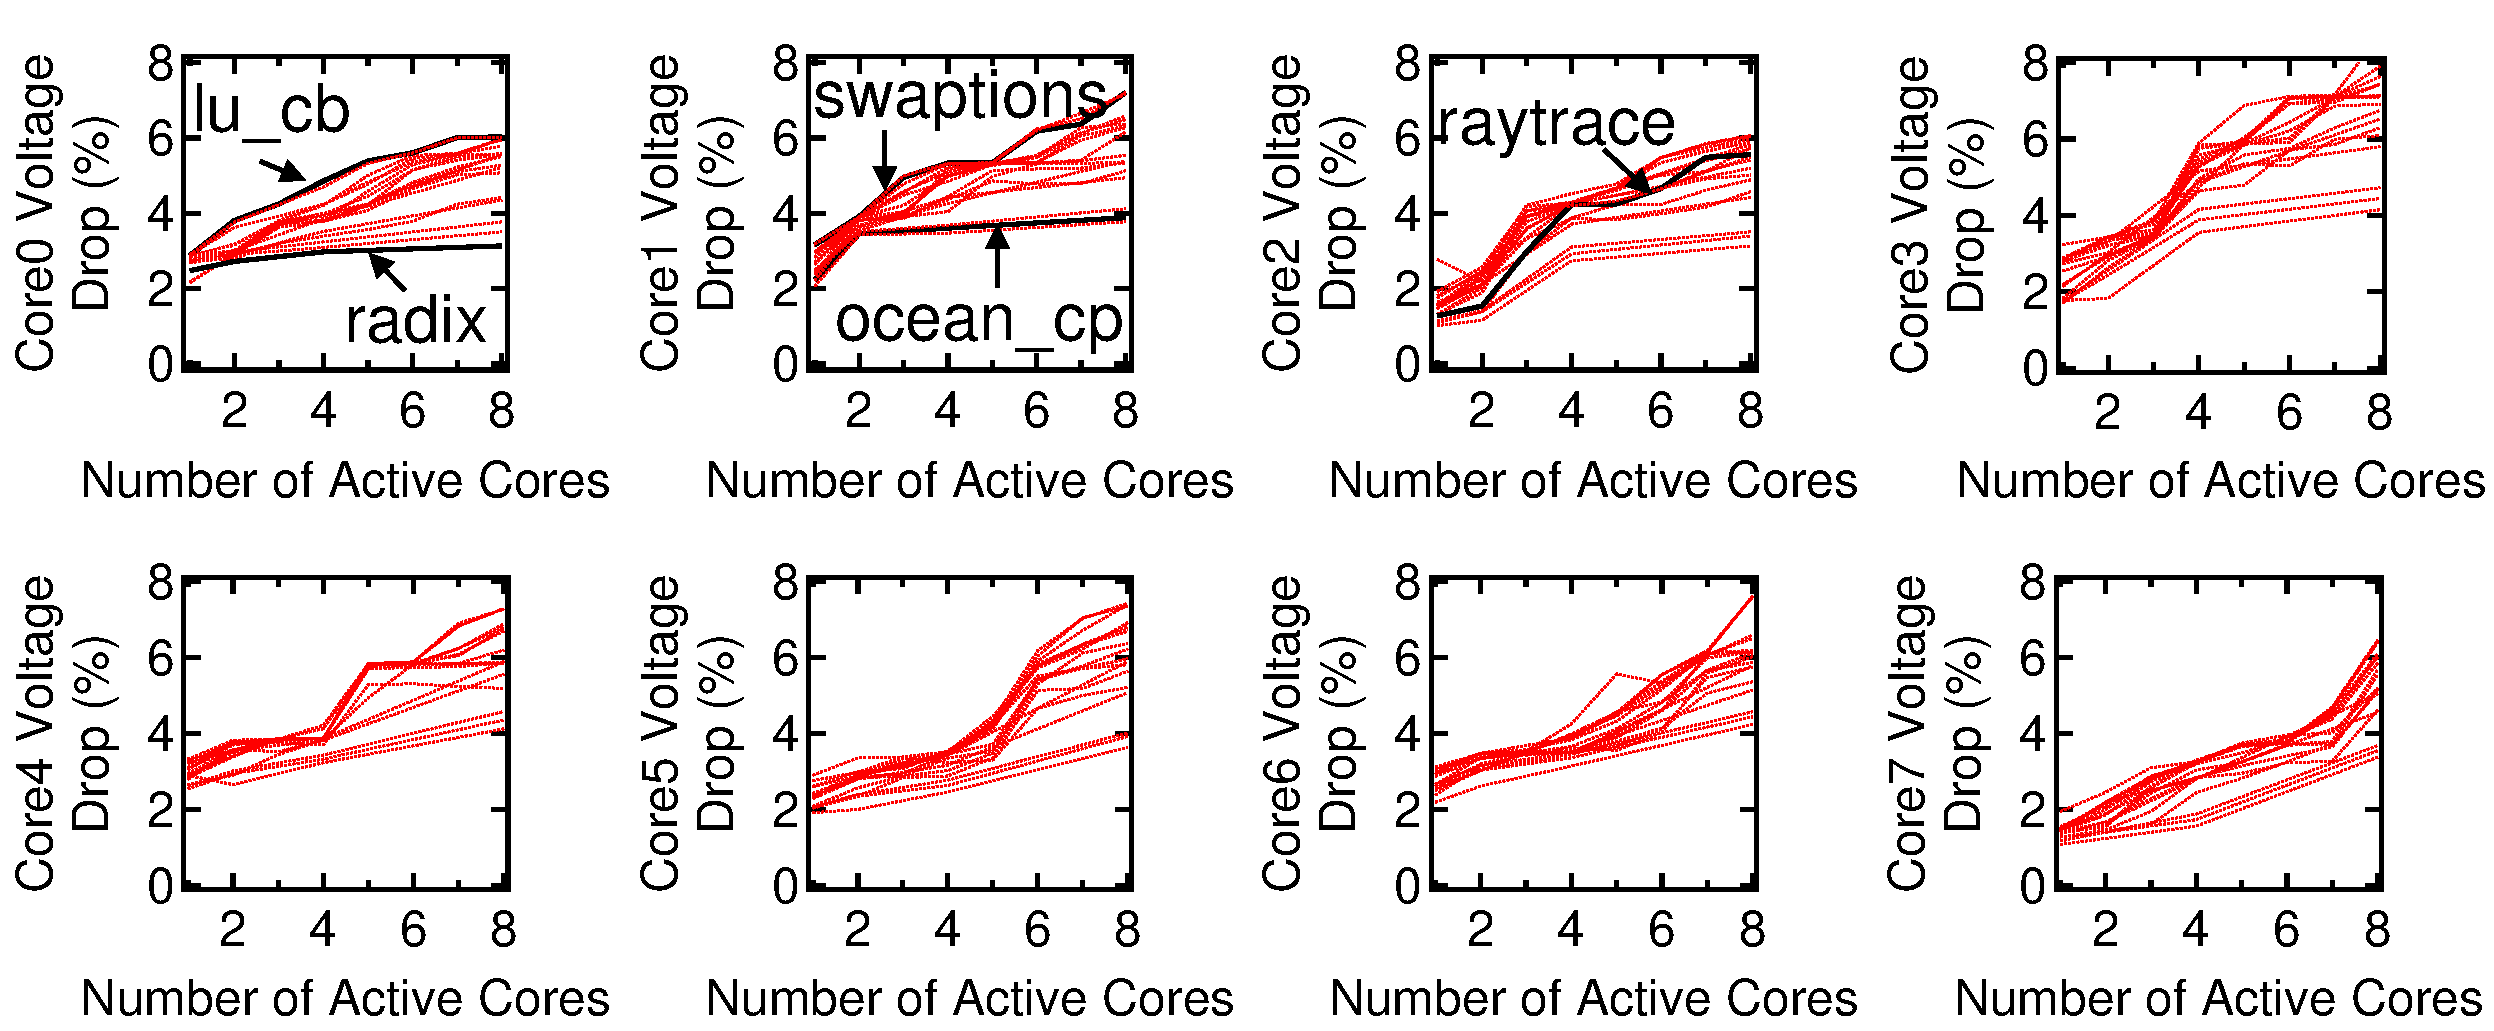
\includegraphics[trim=0 0 0 0,clip,height=1.5in]{graphs/voltage/cpm_scale_variation.pdf}
    \captionsetup{width=0.95\textwidth}
    \vspace{-0.2cm}
    \caption{On-chip voltage drop analysis across cores under different workloads.}
  \label{fig:cpm-variation} 
  \end{minipage}
\hspace{0cm}
  \begin{minipage}{0.47\linewidth}
    \centering
    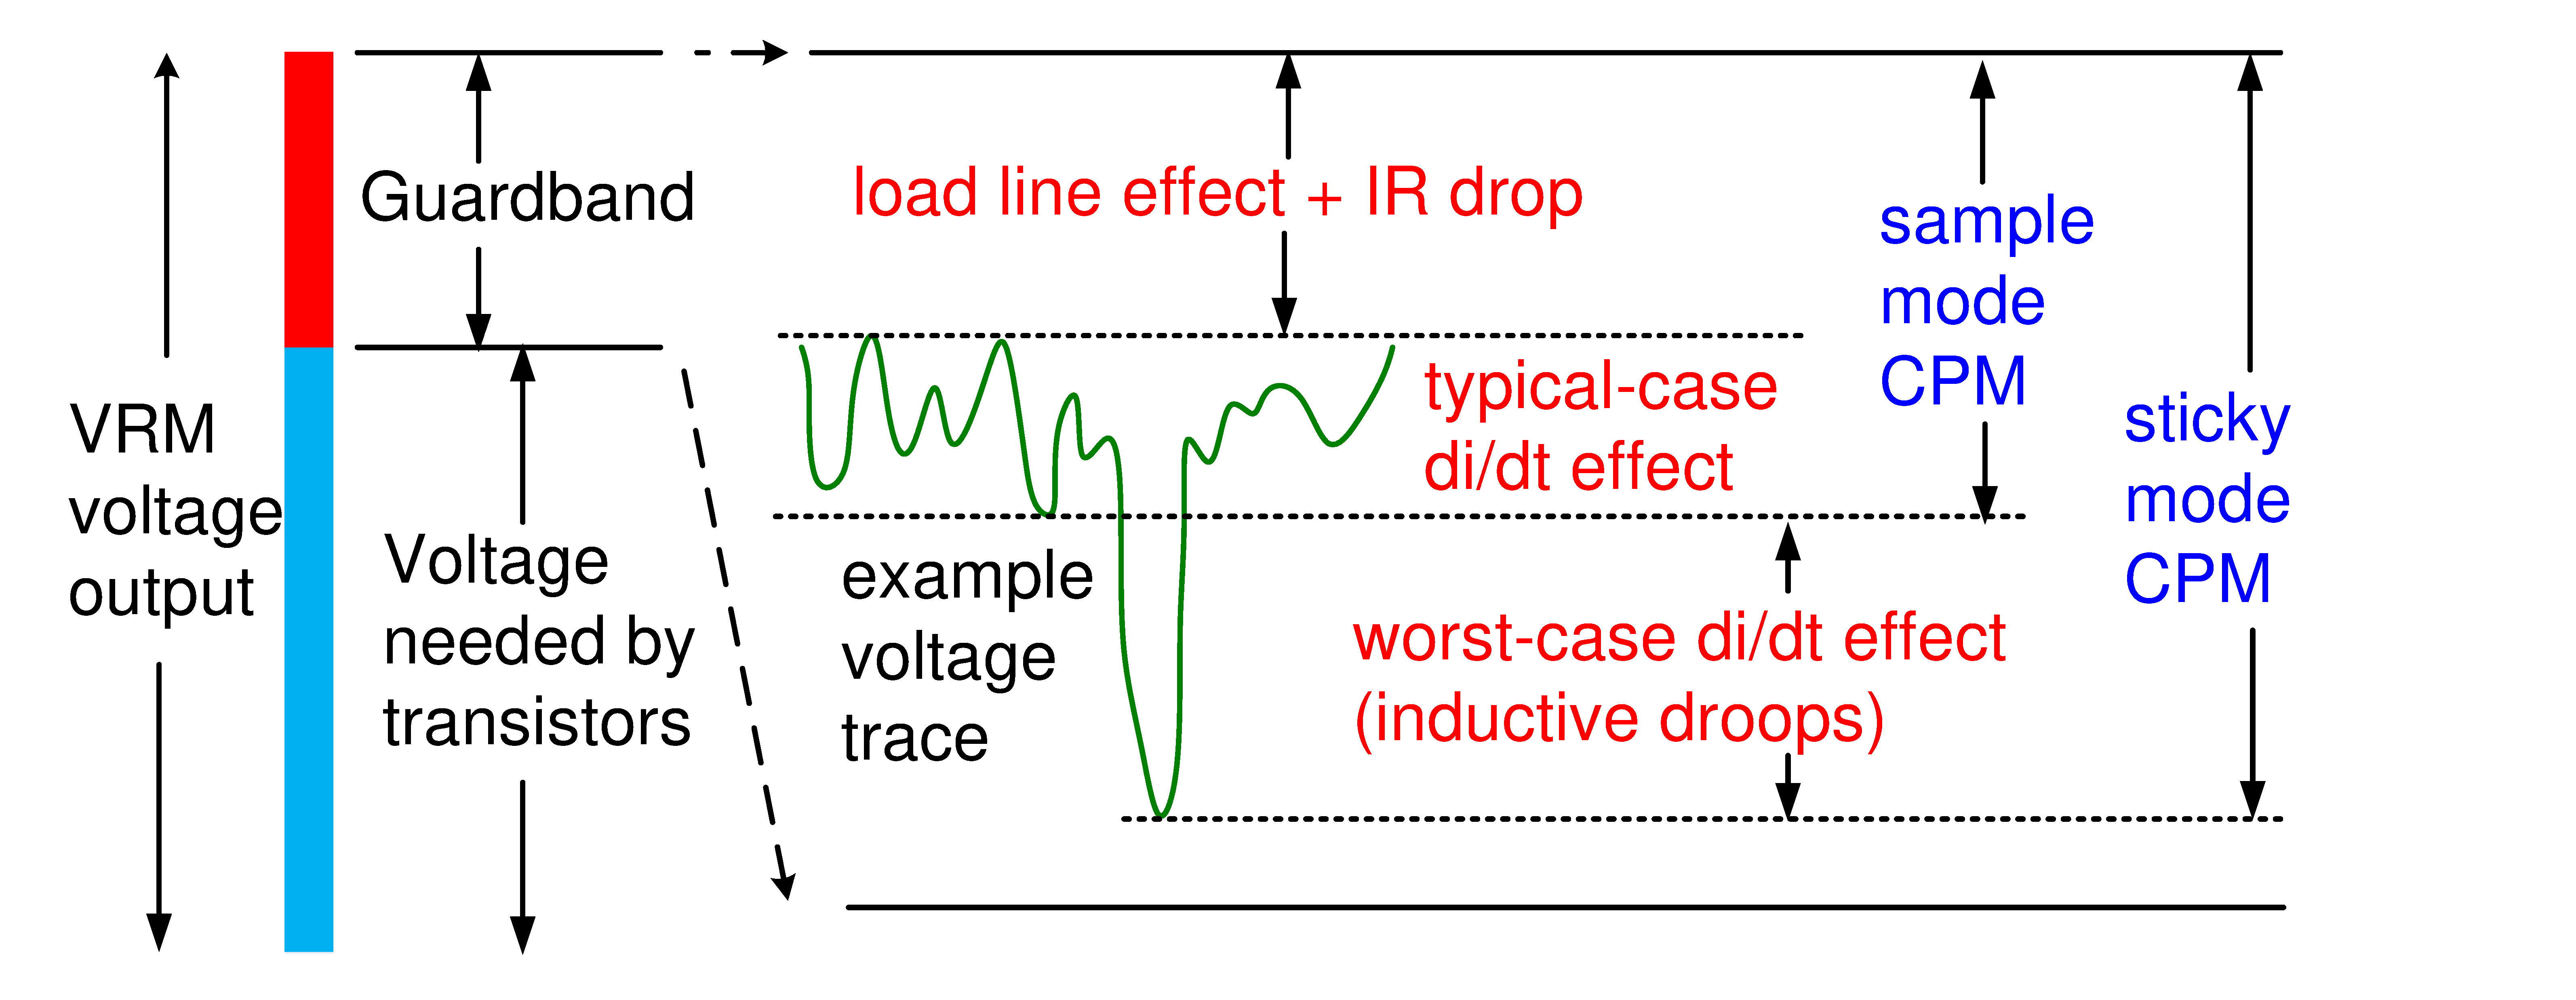
\includegraphics[trim=0 0 0 0,clip,height=1.5in]{graphs/voltage/noise_components.pdf}
    \captionsetup{width=0.95\textwidth}
    \vspace{-0.3cm}
    \caption{Voltage drop component analysis, including $di/dt$ droop, IR drop and the loadline effect.}
    \label{fig:vnoise-component} 
  \end{minipage}
\end{figure*}

\Fig{fig:cpm2volt} lets us establish a direct relationship between CPM and on-chip voltage. We observe a near-linear relationship between the two variables under each frequency. Therefore, with a linear fit, we can determine each CPM bit's significance. On average, one CPM output value corresponds to 21~mV of on-chip voltage. On this basis, we can estimate the magnitude of on-chip voltage drop during any 32~ms interval. For instance, if the measured CPM output drops from eight to four, the estimated on-chip voltage has dropped by 84~mV. 

\Fig{fig:cpmsensitivity} shows the sensitivity of the CPMs within each processor core. Although we see a near-linear relationship between frequency and all the CPMs, there is variation among the CPMs in each core and between cores. For instance, CPMs in Core~2,~6,~7 have steadier sensitivity compared to Core~1,~3,~5. The latter have higher distribution across CPMs. We attribute this behavior to process variation and CPM calibration error, as explained by prior work~\cite{floyd2013runtime}.

To ensure the robustness of our measurement results, we considered both repeatability and temperature effects. We repeated our experiment on another socket in the same server, and the result conforms to the same trend shown in~\Fig{fig:cpm2volt}. We observe that chip temperature varies between $27$\textdegree C at the lowest frequency to $38$\textdegree C at the highest. Internal benchmark runs show such temperature variation does not have significant influence over CPM readings, and thus we can draw general conclusions from~\Fig{fig:cpm2volt}.

\subsection{On-chip Voltage Drop Analysis}
\label{sec:voltage:rootcause:vdrop-analysis}

Using our on-chip voltage drop measurement setup, we quantify the magnitude of the on-chip voltage drop to explain the general core scaling trends seen in~\Sec{sec:characterization}. It is important to understand what factors, and more importantly how those factors, impact the efficiency of active timing margin as more cores are activated. 

\Fig{fig:cpm-variation} shows the measured results for the voltage drop across different cores within the processor, ranging from Core~0 through Core~7. The cores are spatially located in the same order as they appear on the physical processor~\cite{zyuban2013ibm}. The $y$-axis is the percentage of on-chip voltage drop from the nominal. Given the magnitude of voltage drop and knowledge about the system's nominal operating voltage, we can determine the percentage change. The $x$-axis indicates the total number of simultaneously active cores, specifically as they are activated in succession from core 0 to 7. Keeping consistent with \Fig{fig:workloadvariation}, each line in the subplots corresponds to one workload from PARSEC and SPLASH-2. Each subplot shows a particular core's characteristics with respect to every other (active or inactive) core in the processor. 

\Fig{fig:cpm-variation} lets us understand several important factors that affect active timing margin's efficiency. First, voltage drop increases as more cores are activated. For all workloads, voltage drop increases from about 2\% to 8\% as the number of active cores increases. The trend is similar to the diminishing benefits seen previously in the power and frequency improvement in \Fig{fig:workloadvariation}. As the magnitude of voltage drop increases, timing margin decreases and thus active timing margin's efficiency decreases at higher loads. 

\begin{figure*}[t]
     \subfloat[raytrace.] {
        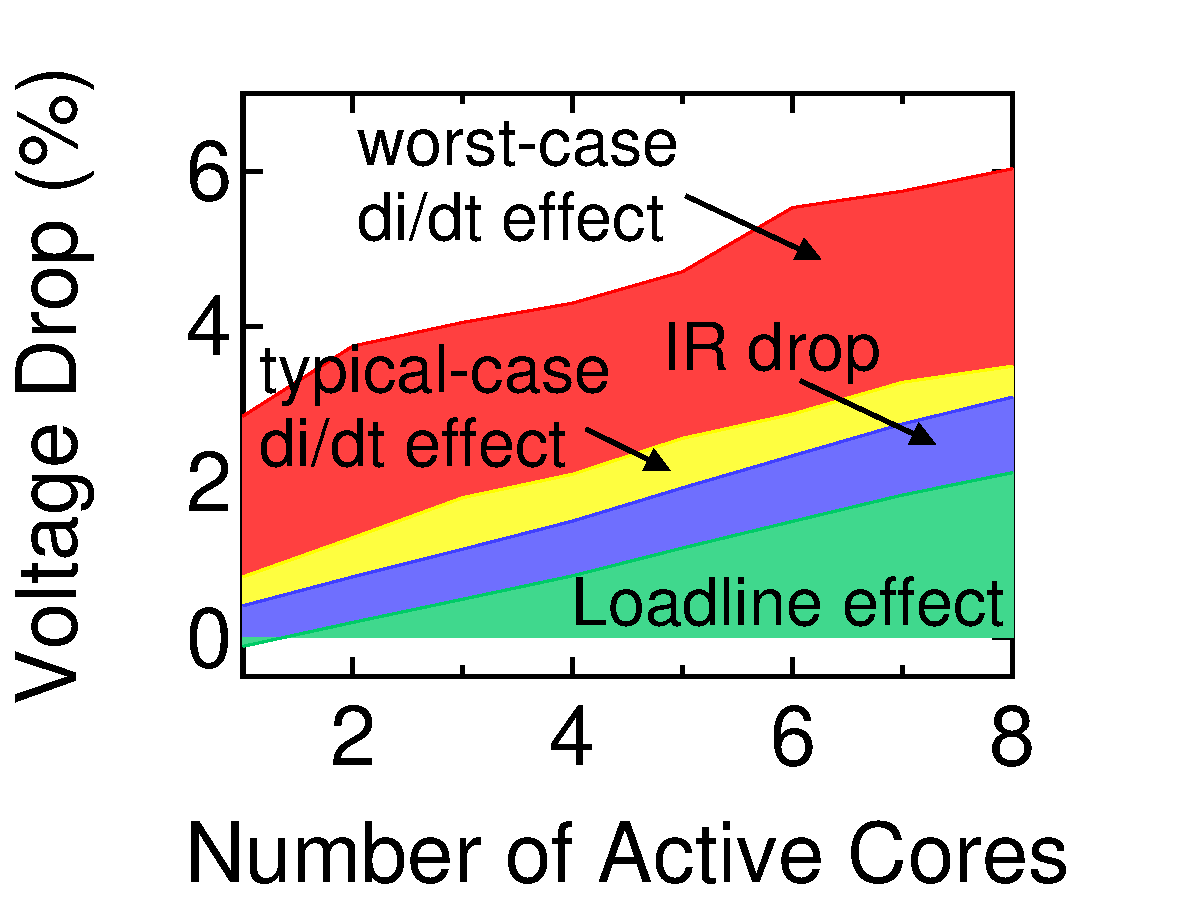
\includegraphics[trim=0 0 0 0,clip,width=.2\linewidth]{graphs/voltage/current_raytrace.pdf}
        \label{fig:raytrace_ir} 
      }
      \hspace*{-.1in}
      \subfloat[barnes.] {
        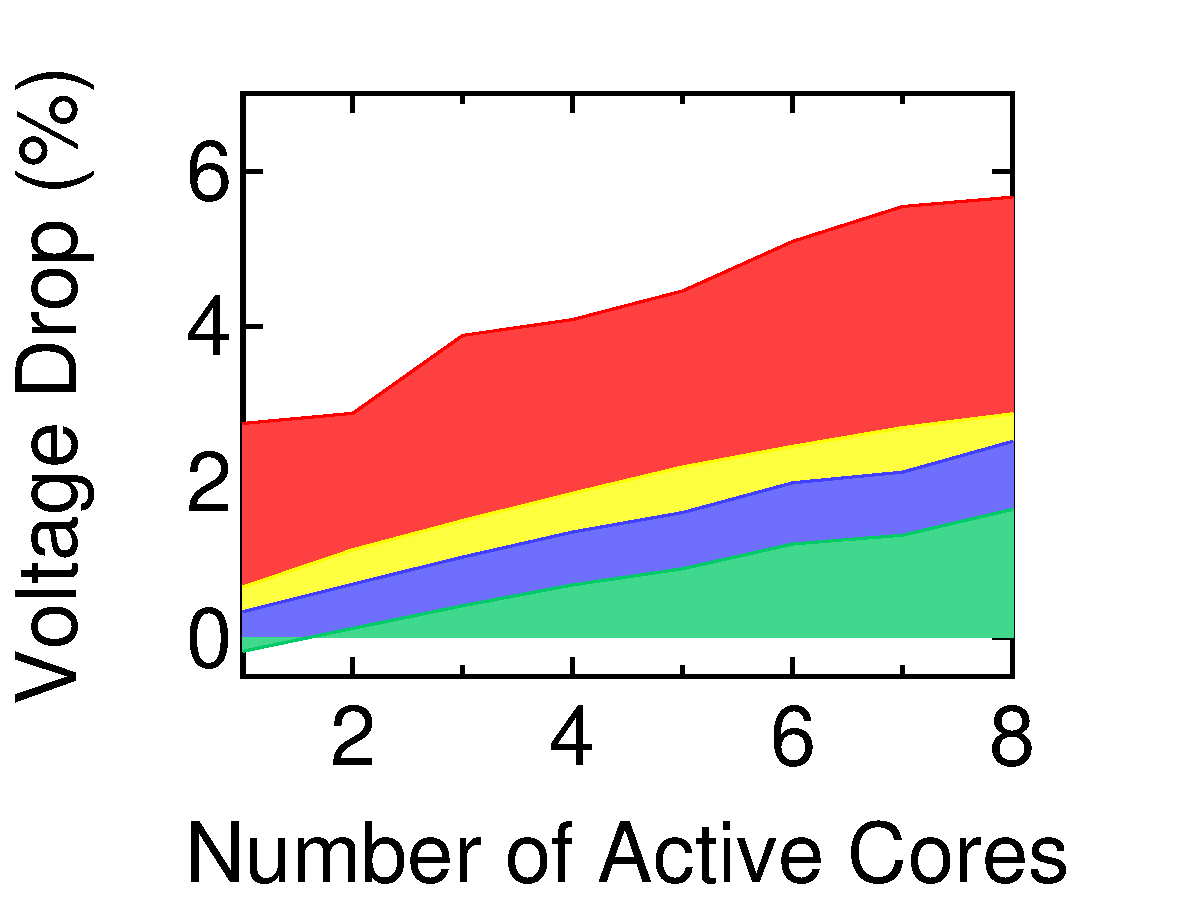
\includegraphics[trim=0 0 0 0,clip,width=.2\linewidth]{graphs/voltage/current_barnes.pdf}
        \label{fig:barnes_comp} 
      }
      \hspace*{-.1in}
      \subfloat[blackscholes.] {
        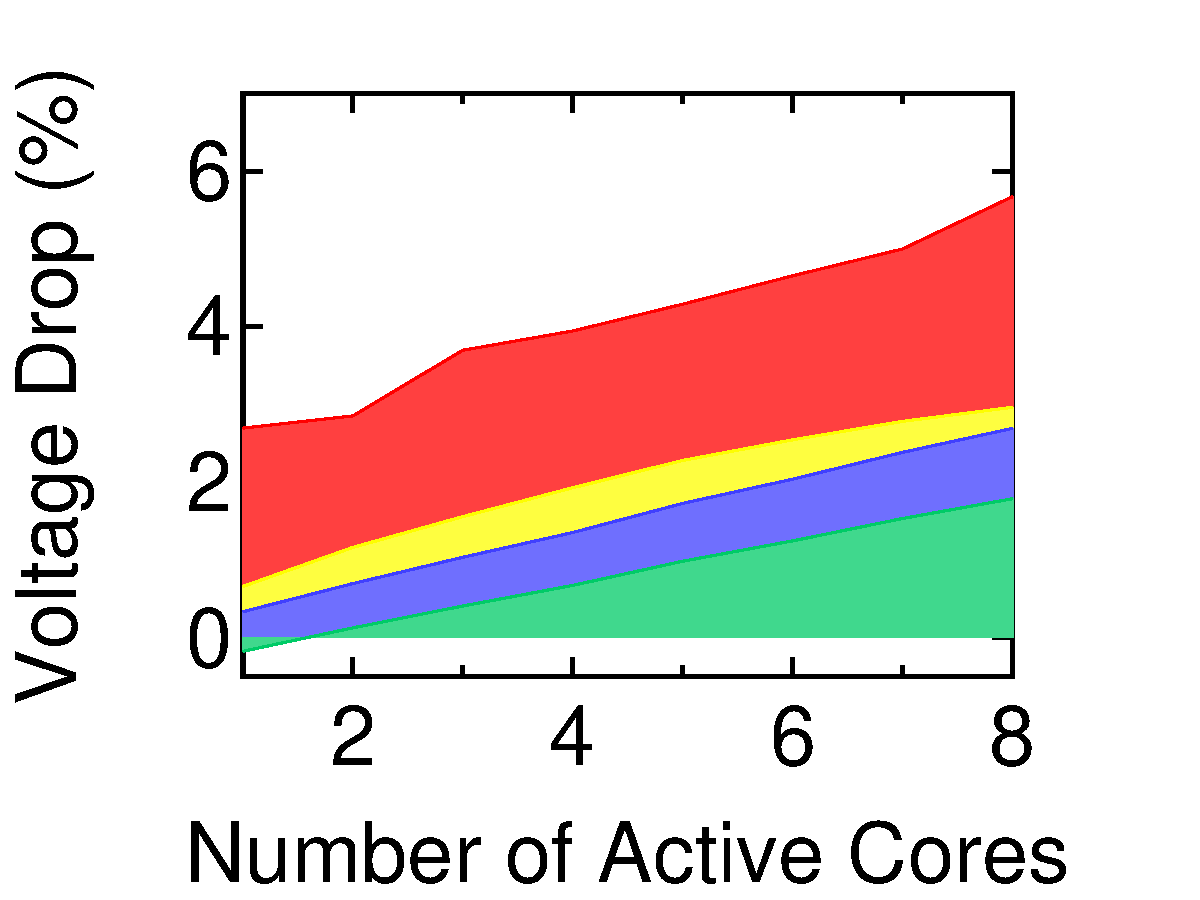
\includegraphics[trim=0 0 0 0,clip,width=.2\linewidth]{graphs/voltage/current_blackscholes.pdf}
        \label{fig:blackscholes_comp} 
      }
      \hspace*{-.1in}
      \subfloat[bodytrack.] {
        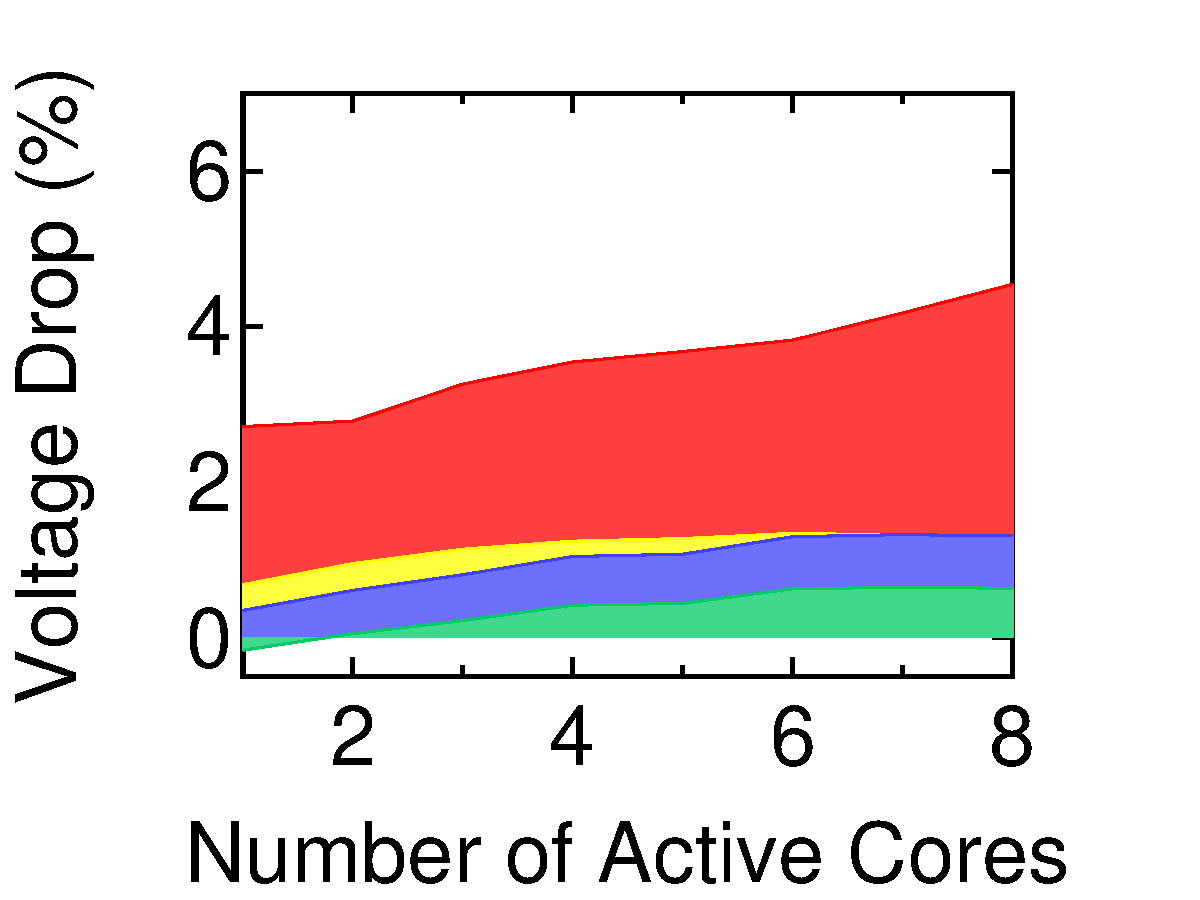
\includegraphics[trim=0 0 0 0,clip,width=.2\linewidth]{graphs/voltage/current_bodytrack.pdf}
        \label{fig:bodytrack_comp} 
      }
     \hspace*{-.1in}
      \subfloat[ferret.] {
        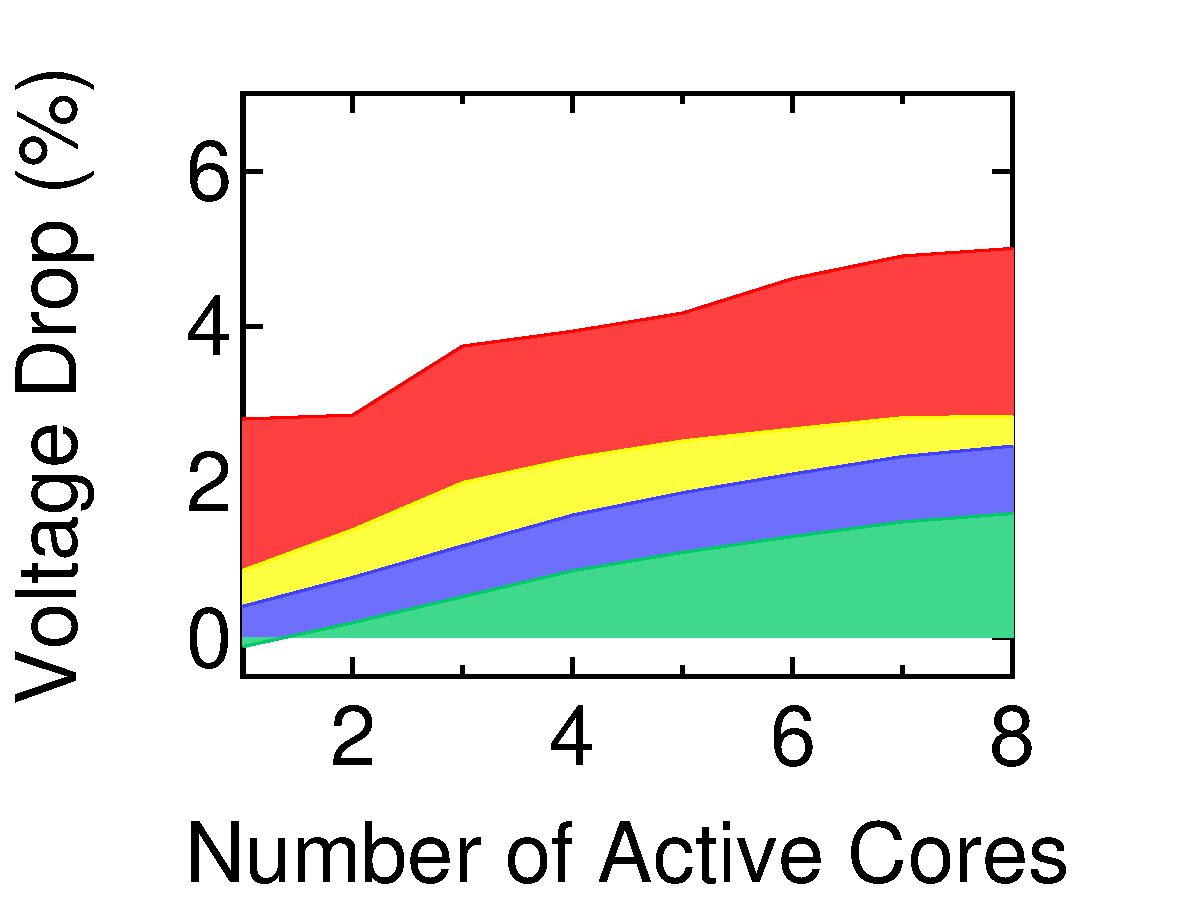
\includegraphics[trim=0 0 0 0,clip,width=.2\linewidth]{graphs/voltage/current_ferret.pdf}
        \label{fig:ferret_comp} 
      }
\vspace*{-.15in}
      \hspace*{-.05in} 
      \subfloat[lu\_ncb.] {
        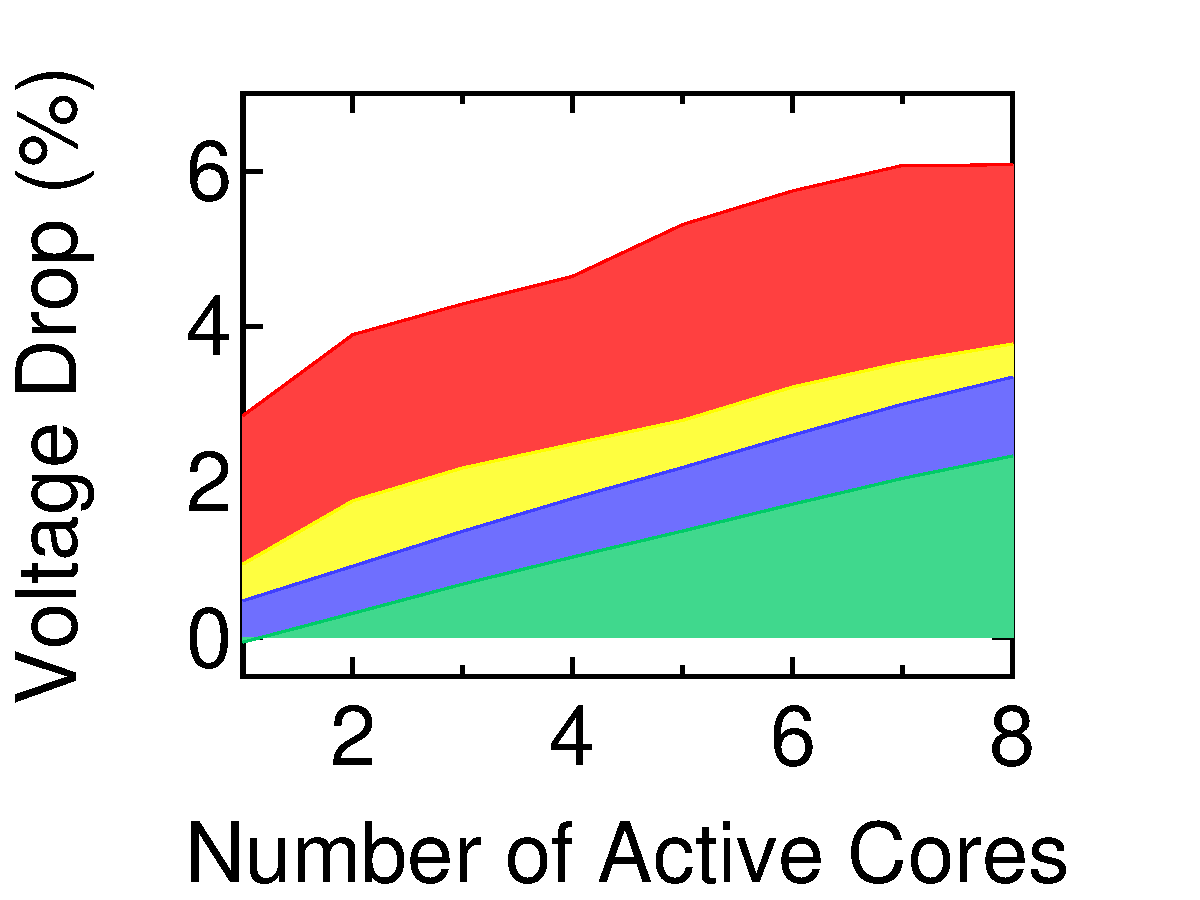
\includegraphics[trim=0 0 0 0,clip,width=.2\linewidth]{graphs/voltage/current_lu_ncb.pdf}
        \label{fig:lu_ncb_comp} 
      }
      \hspace*{-.1in} 
      \subfloat[ocean\_cp.] {
        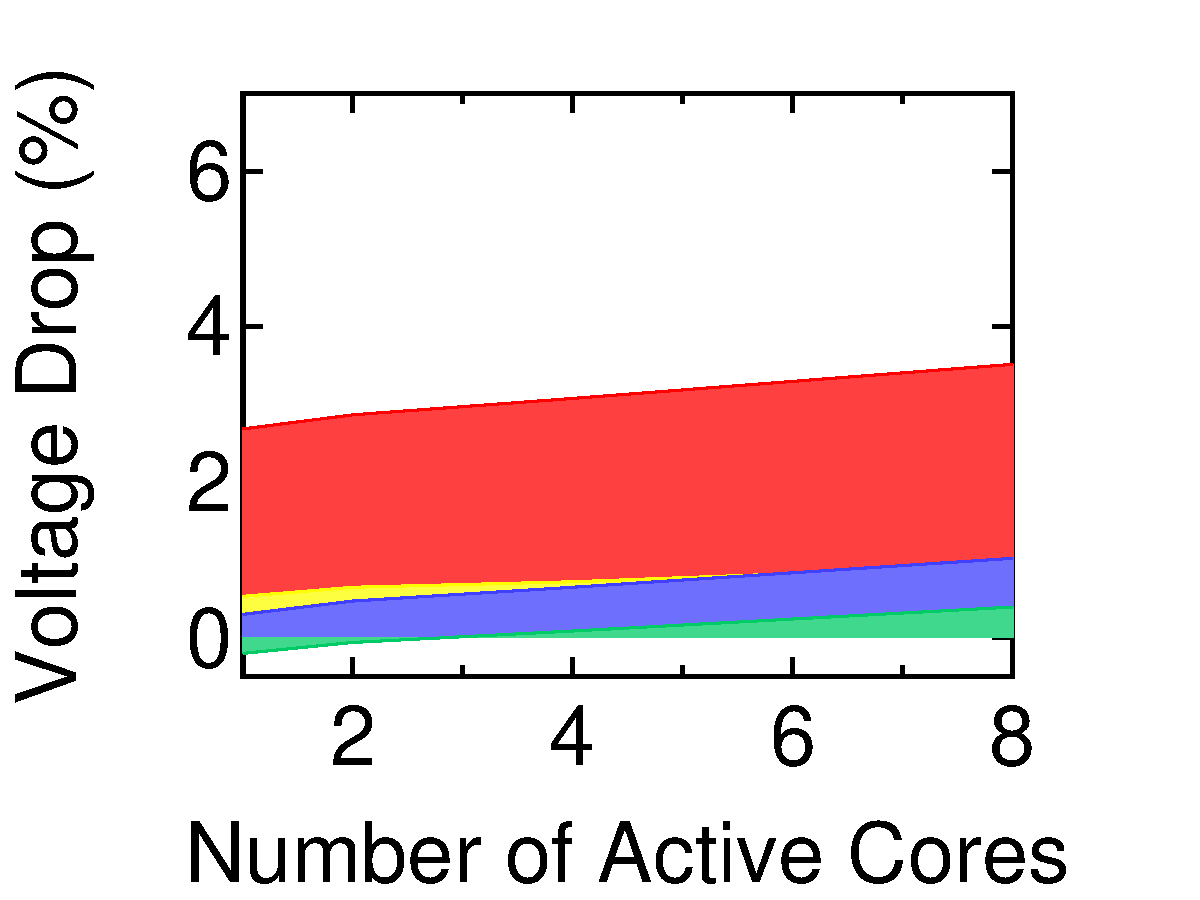
\includegraphics[trim=0 0 0 0,clip,width=.2\linewidth]{graphs/voltage/current_ocean_cp.pdf}
        \label{fig:ocean_cp_comp} 
      }
      \hspace*{-.1in} 
      \subfloat[swaptions.] {
        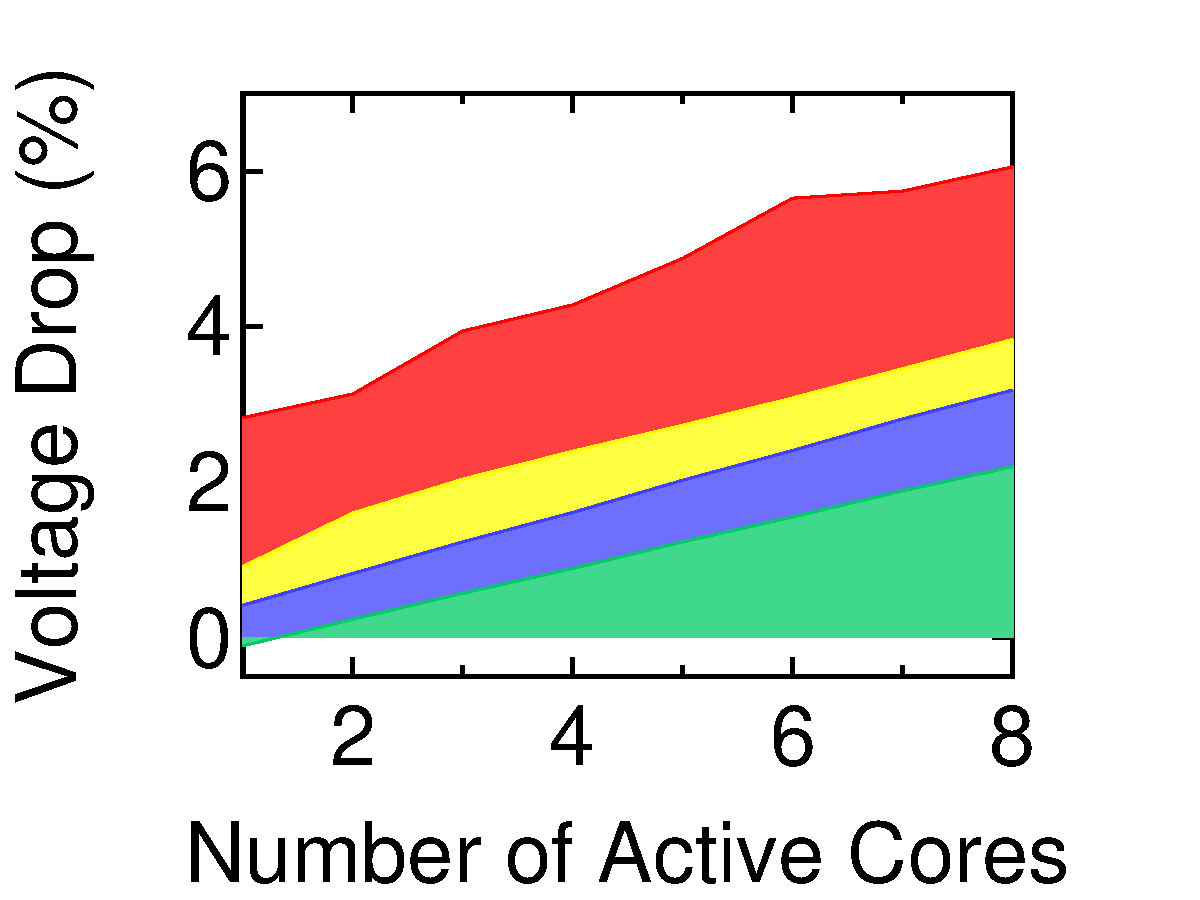
\includegraphics[trim=0 0 0 0,clip,width=.2\linewidth]{graphs/voltage/current_swaptions.pdf}
        \label{fig:swaptions_comp} 
      }
      \hspace*{-.1in} 
      \subfloat[vips.] {
        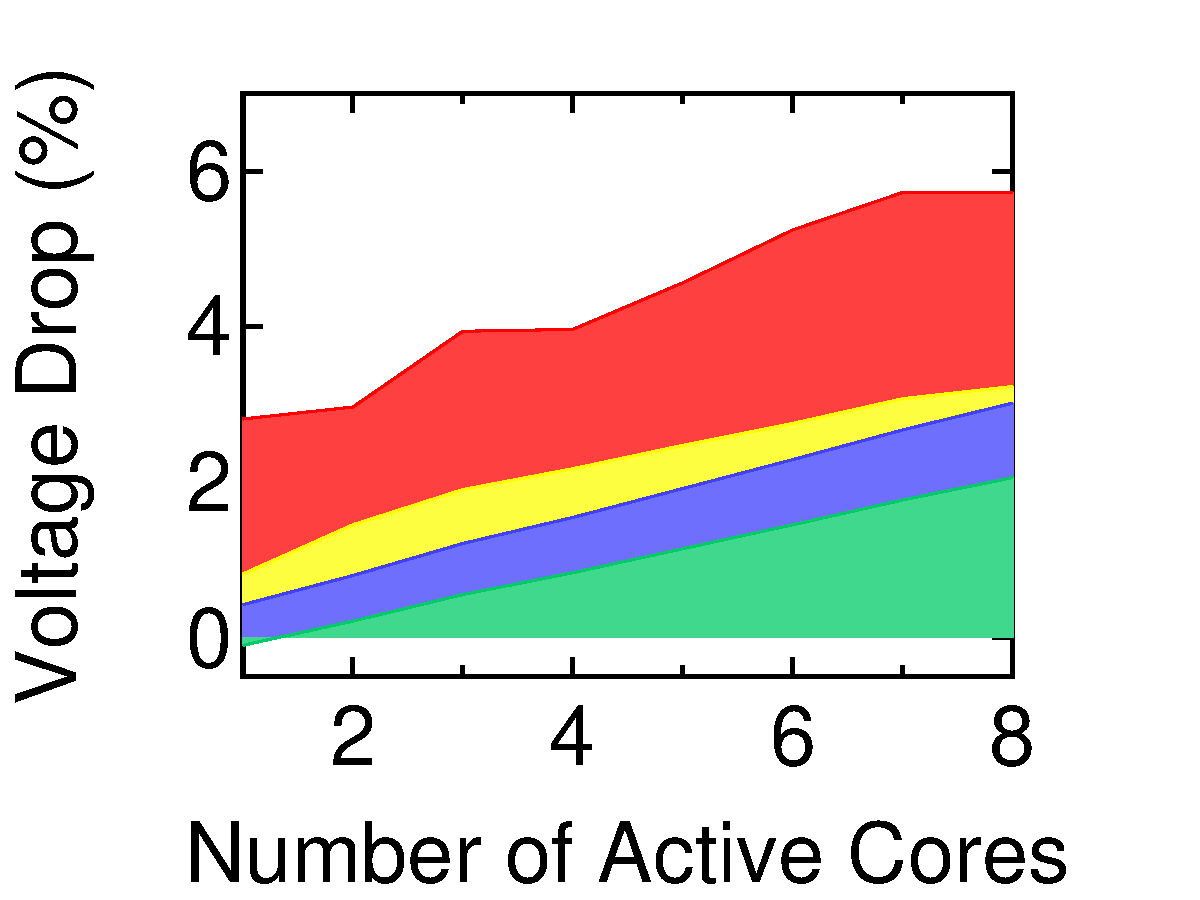
\includegraphics[trim=0 0 0 0,clip,width=.2\linewidth]{graphs/voltage/current_vips.pdf}
        \label{fig:vips_comp} 
      }
      \hspace*{-.1in} 
      \subfloat[water\_nsquared.] {
        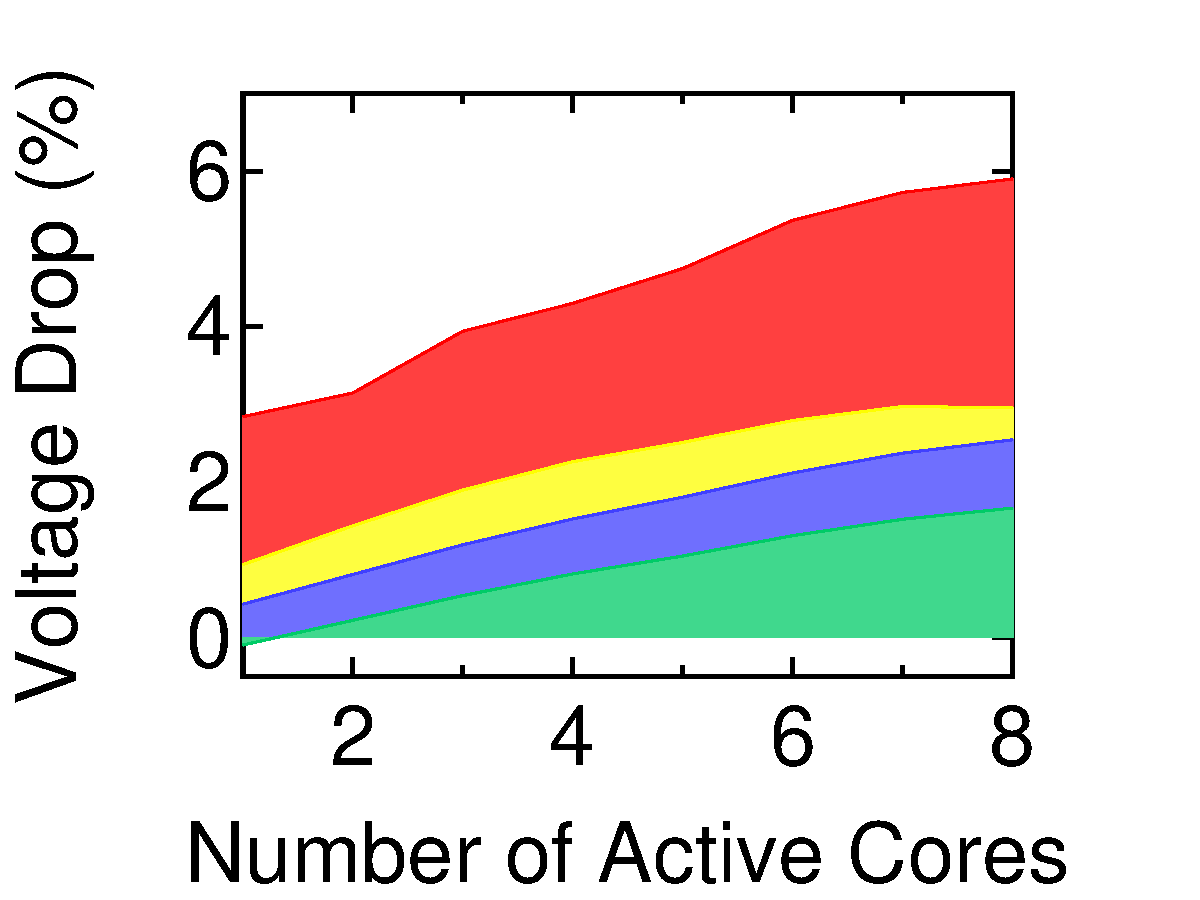
\includegraphics[trim=0 0 0 0,clip,width=.2\linewidth]{graphs/voltage/current_water_nsquared.pdf}
        \label{fig:water_nsquared_comp} 
      }
    \caption{Different components of on-chip voltage drop for some PARSEC and SPLASH-2 benchmarks. In general, as more of the processor's cores are activated, voltage drop increases by varying magnitudes across workloads.}
    \label{fig:drop-components} 
\end{figure*}

Second, the increasing on-chip voltage drop trend manifests as chip-wide global behavior because voltage drop affects all cores at the same time, regardless of whether they are idling or actively running a workload. For instance, when cores on the upper row (Core~0 through Core~3) are actively running a workload, they experience voltage drop. Meanwhile, cores in the bottom row also experience voltage drop even though Core~4 through Core~7 are not running any workloads. 

The implications of the second finding are that global effects, such as chip-wide $di/dt$ noise~\cite{gupta2007understanding,miller2012vrsync,bertran2014voltage} and off-chip IR drop, can affect active timing margin's system-wide power-saving efficiency because active timing margin makes decisions on the basis of the worst-case behavior of all cores. In particular, this behavior impacts the power-saving mode because the processor has a single off-chip VRM that will need to supply the highest voltage to match the most demanding core's voltage requirement. So, even if some cores are lightly active, the system may have to forgo their active timing margin benefits to support the activity of the busy core(s). In applications where workload imbalance exists, this can become a major efficiency impediment. 

Third, the on-chip voltage drop's scaling trend, as the number of active cores increases, tends to differ across cores, indicating that voltage drop has localized behavior in addition to the global behavior described previously. For instance, across all the cores the magnitude of voltage drop shifts upward significantly whenever that particular core is activated. For instance, Core~7's voltage drop increases by 2\% when it is activated, as evident in Core~7's voltage drop plot.

More generally, cores that are activated earlier have a higher voltage drop at first, and thereafter their voltage drop begins to saturate and plateau. For instance, Core~0 and Core~1 have a higher voltage drop when Core~0 through Core~3 are activated. These cores' voltage drop increase quickly when the number of active cores is less than four. On the contrary, the voltage drop for Core~4 through Core~7 does not change much while Core~0 through Core~3 are activated, but thereafter their voltage drop increases much more quickly.

Localized effects impact the operation of the per-core frequency-boosting mode. Each POWER7+ core has its own DPLL that can dynamically perform frequency scaling to improve performance when required. However, each core's performance can be boosted only when it is not affected by activity on its neighboring cores. In general, our observations imply that it is easier to boost clock frequency and, hopefully, performance -- at least for computing-bound workloads -- over reducing voltage, because frequency-boosting is largely affected by localized voltage drop. By comparison, the global voltage drop typically tends to have a more pronounced effect on the chip-wide power-saving mode. 

\subsection{Decomposing the On-chip Voltage Drop}
\label{sec:voltage:rootcause:vdrop-decompose}

To understand how workload heterogeneity affects the power-saving and frequency-boosting modes when all cores are active, we must understand why the on-chip voltage drop varies significantly from one workload to another with an increasing number of cores. For example, in \Fig{fig:cpm-variation} \benchmark{lu\_cb}'s voltage drop increases more quickly compared to \benchmark{radix}, whose voltage drop does not change much as the number of active cores increases.  We decompose the on-chip voltage drop into its three primary components (see \Fig{fig:vnoise-component}): worst-case $di/dt$ noise, also called voltage droops due to sudden current surges caused by microarchitecture activities; typical-case $di/dt$ noise due to regular current ripples; and passive voltage drop due to IR drop across the PDN and the loadline effect~\cite{lefurgy2011active} at the VRM.

We use a mixture of current sensing techniques and CPM measurements to decompose the voltage drop. To measure passive voltage drop (i.e., loadline effect + IR drop), we use VRM's current sensors. The IR drop and loadline effects are quantified using a heuristic equation verified against hardware measurements. The input to the equation is the current going from the VRM into the POWER7+ processor, sampled periodically.

We use CPMs to calculate the magnitude of typical and worst-case voltage noise. To get the typical $di/dt$ value, we run the CPMs in sample mode to acquire an immediate CPM reading, and after converting the CPM output into voltage, we subtract the passive component from it. To get the worst-case $di/dt$ value, we run the CPMs in sticky mode to acquire the largest voltage droop seen in the past 32~ms and subtract it from the long-term average measured in sample mode. 

We select several representative benchmarks from previously discussed data and decompose their on-chip voltage drop into $di/dt$ noise and passive drop in \Fig{fig:drop-components}. The subplots are in the form of a stacked area chart, showing the trend as more cores are progressively activated. Only Core~0 data simplifies the presentation of our analysis, although we have verified that the conclusions described in the following paragraphs hold true for the other cores as well.

By analyzing the data, we conclude that passive voltage drop, including IR drop across PDN and VRM's loadline is the dominant factor contributing to increasing voltage drop. Intuitively, these two passive effects have the most direct influence over active timing margin's behavior because they always exist steadily during execution as compared to $di/dt$ noise.

\begin{figure*}[t]
\centering
   \subfloat[] {
    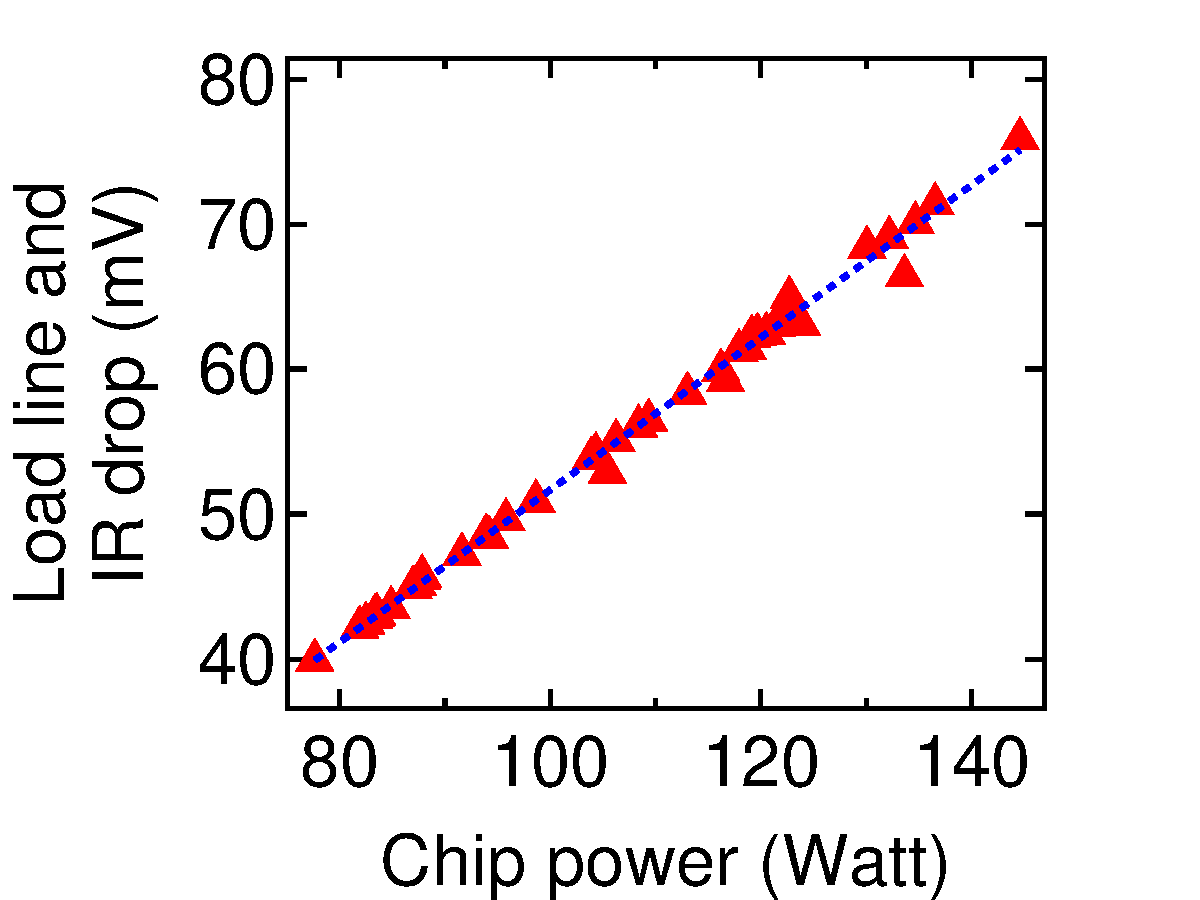
\includegraphics[trim=0 0 20 0,clip, height=1.25in]{graphs/voltage/pwr_loadline.pdf}
    \label{fig:pwr-loadline} 
  }
  \subfloat[] {
    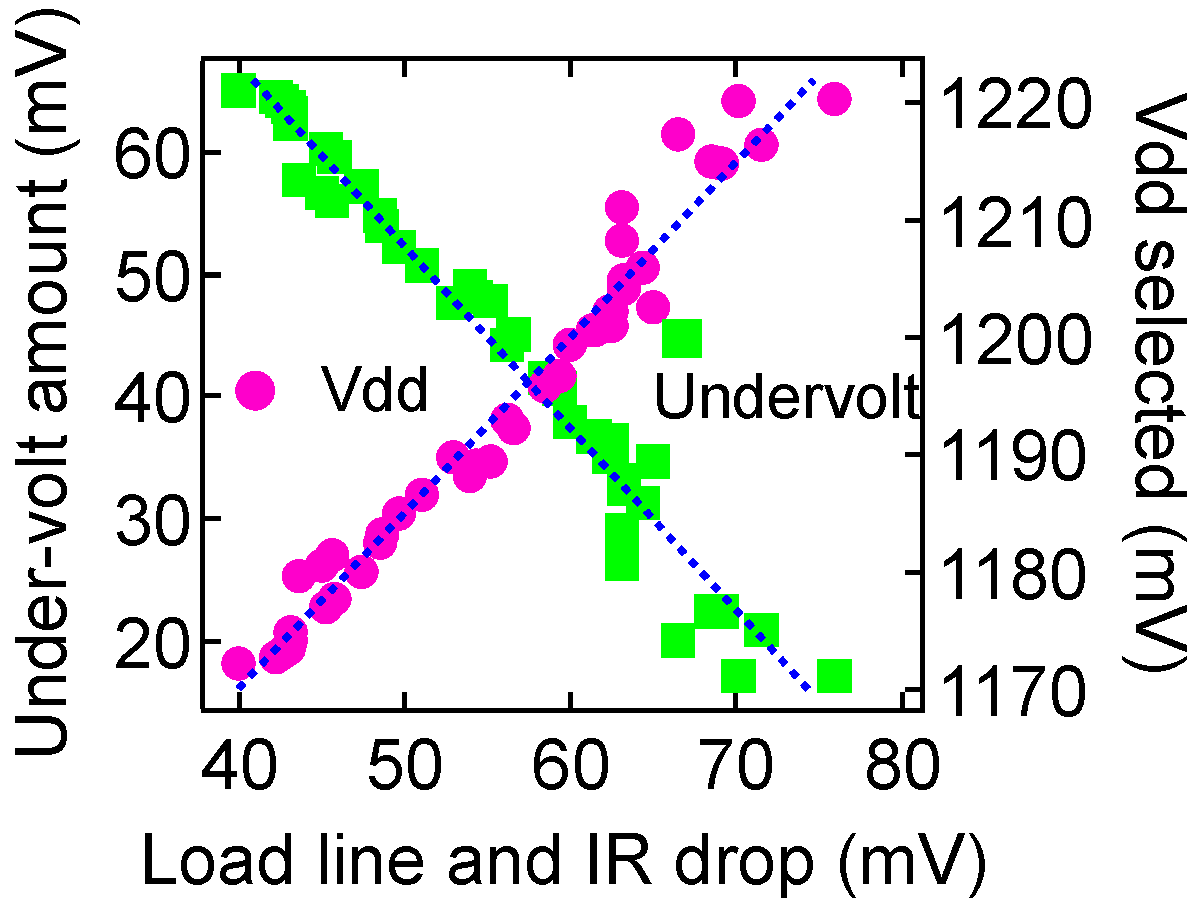
\includegraphics[trim=0 0 -50 0,clip,height=1.25in]{graphs/voltage/loadline_vdd.pdf}
    \label{fig:line-vdd} 
  }
  \subfloat[] {
    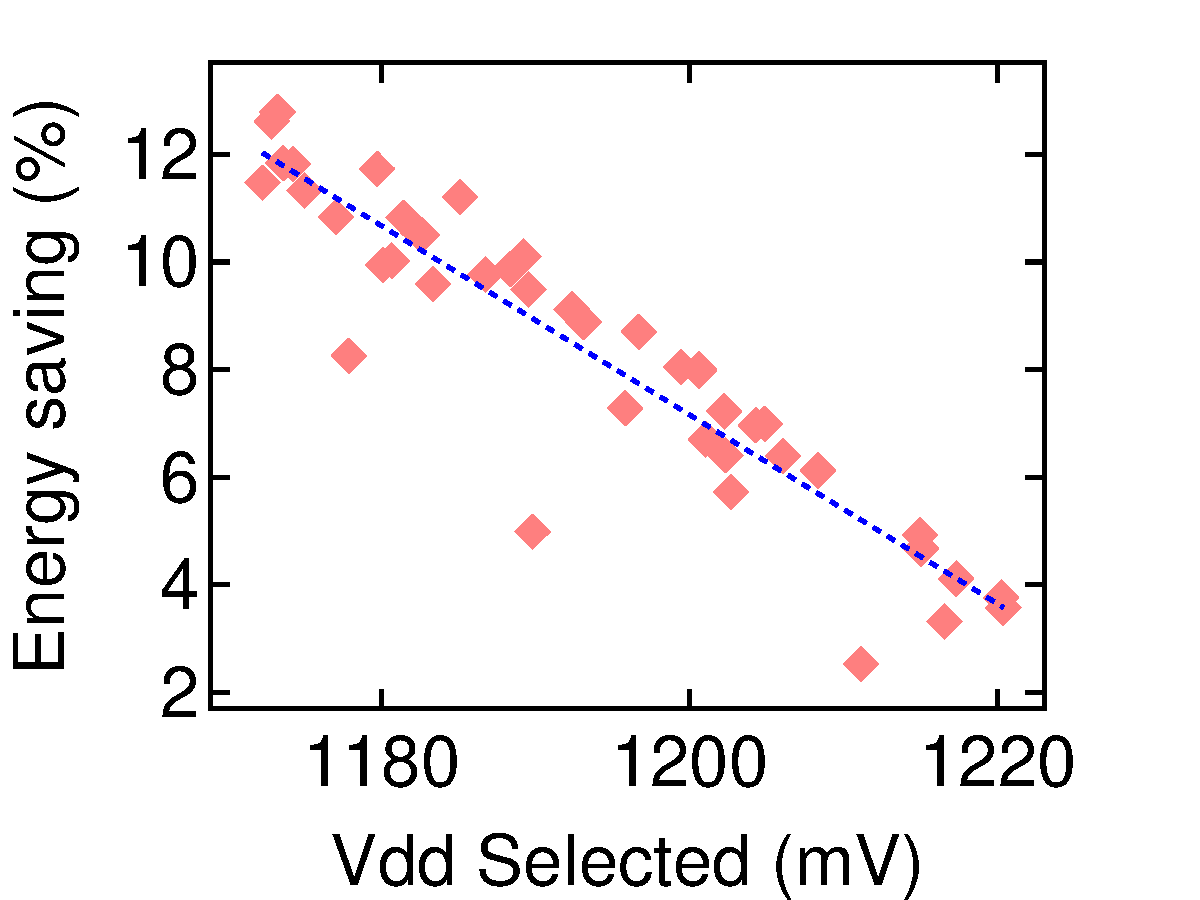
\includegraphics[trim=0 0 20 0,clip,height=1.25in]{graphs/voltage/vdd_saving.pdf}
    \label{fig:vdd-saving} 
  }
  \subfloat[] {
    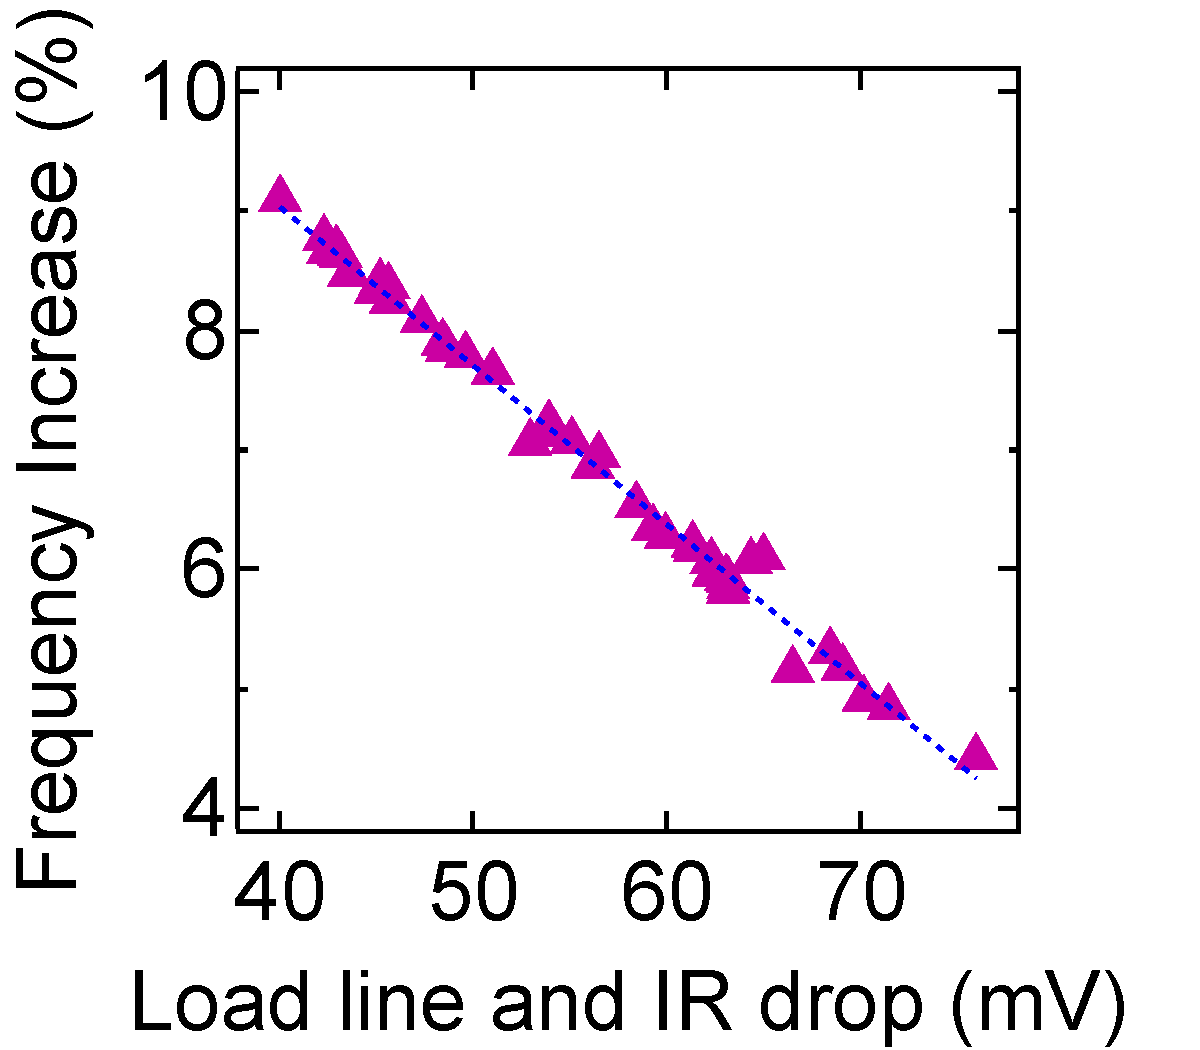
\includegraphics[trim=0 0 20 0,clip,height=1.25in]{graphs/voltage/loadline_freq.pdf}
    \label{fig:line-freq} 
  }
  \caption{Power-intensive workloads induce large loadline and IR drop, which severely limits the active timing margin system's undervolting capability, and thus impacts the system's overall power-saving potential.}
  \label{fig:ldir-proof}
\end{figure*}

As we scale the number of active cores, the worst-case $di/dt$ noise increases slightly across all of the benchmarks, and typical-case $di/dt$ noise decreases. For instance, the worst-case $di/dt$ noise growth is noticeable in \benchmark{bodytrack}, \benchmark{vips} and \benchmark{water\_nsquared}. When multiple cores are active simultaneously, they can have synchronous behavior, or random alignment, that can cause large and sudden current swings leading to voltage droops~\cite{reddi2010voltage,miller2012vrsync,kim2012audit}. However, our droop frequency analysis (not shown here) indicates that such large worst-case droops occur infrequently. On the contrary, typical-case $di/dt$ noise gets smaller when core count scales. With more active cores, microarchitectural activities stagger among different cores, which can lead to noise smoothing ~\cite{miller2012vrsync,reddi2010voltage}.

Compared to $di/dt$ noise, we find a clear scale-up trend of passive voltage drop from~\Fig{fig:drop-components}, and it contributes most to the scale-up of total voltage drop. IR drop and loadline effects increase almost linearly with the number of active cores because the passive voltage drop is caused by processor current draw, which is further determined by chip power. When more cores are used, the whole chip consumes more dynamic power and will lead to higher IR drop and loadline effects.

Because active timing margin can deal with occasional $di/dt$ voltage droops by slowing down frequency quickly, the rare voltage drop caused by this effect does not strongly influence the power-saving and frequency-boosting capability of active timing margin, even though they consume a significant portion of the total voltage guardband. Thus, we believe passive voltage drop is the main source of impact to active timing margin's efficiency. 

We confirm that loadline and IR drop cause active timing margin's inefficiency at full load by quantifying the relationship between their voltage drop under static guardbanding with respect to the system's two optimization modes: power saving (i.e., undervolting) and frequency boosting (i.e., overclocking). \Fig{fig:ldir-proof} shows the causal relationship between workload power consumption, loadline and IR drop, and the active timing margin's two modes. To ensure we have enough data points, we consider 27 SPECrate workloads on top of the existing 17 PARSEC and SPLASH-2 workloads used before. Each point represents the data we experimentally measured for one benchmark.

In~\Fig{fig:ldir-proof}, across all the subfigures, we see a strong correlation between passive voltage drop and the power-saving and frequency-boosting modes. \Fig{fig:pwr-loadline} shows a strong linear relationship between power and passive voltage drop. \Fig{fig:line-vdd} shows when a workload has a high loadline and IR drop, the voltage guardband is highly utilized, and so active timing margin has less room for undervolting. Thus, the voltage selected by active timing margin is higher. The result is fewer energy savings for high-power workloads, as the data in~\Fig{fig:vdd-saving} demonstrates. The same holds true for active timing margin's frequency-boosting mode. Here as well, a high loadline and IR drop reduce the timing margin; thus, the DPLL has limited room left to overclock the frequency as shown in \Fig{fig:line-freq}.

\section{Architecture \/ Scheduling Optimization}
\label{sec:voltage:opt}

We propose system-level scheduling techniques to improve the benefits of active timing margin. Our scheduler's overarching goal is to minimize the impact that loadline and IR drop have on an active timing margin processor's power and performance efficiency. We demonstrate \emph{active timing margin scheduling} (AMS) int \Sec{sec:voltage:opt:loadline}, and evaluates its effect in runtime power reduction in \Sec{sec:voltage:opt:result}

In a multi-socket server, conventional wisdom says to consolidate workloads onto fewer processors so that the idle processor can be shut down to eliminate wasted power~\cite{murthy2013linux,lo2014towards,leverich2014reconciling}. However, this principle does not apply to servers with active timing margin and per-core power-gating capability. Our measured results show consolidation actually leads to higher power o these systems. We propose loadline borrowing to maximize active timing margin's power-saving benefits for the underlying processors. Compared to workload consolidation, loadline borrowing achieves up to 12\% power savings.

\begin{figure}[!b]
\centering
\vspace*{-10pt}
\subfloat[Workload consolidation.] {
    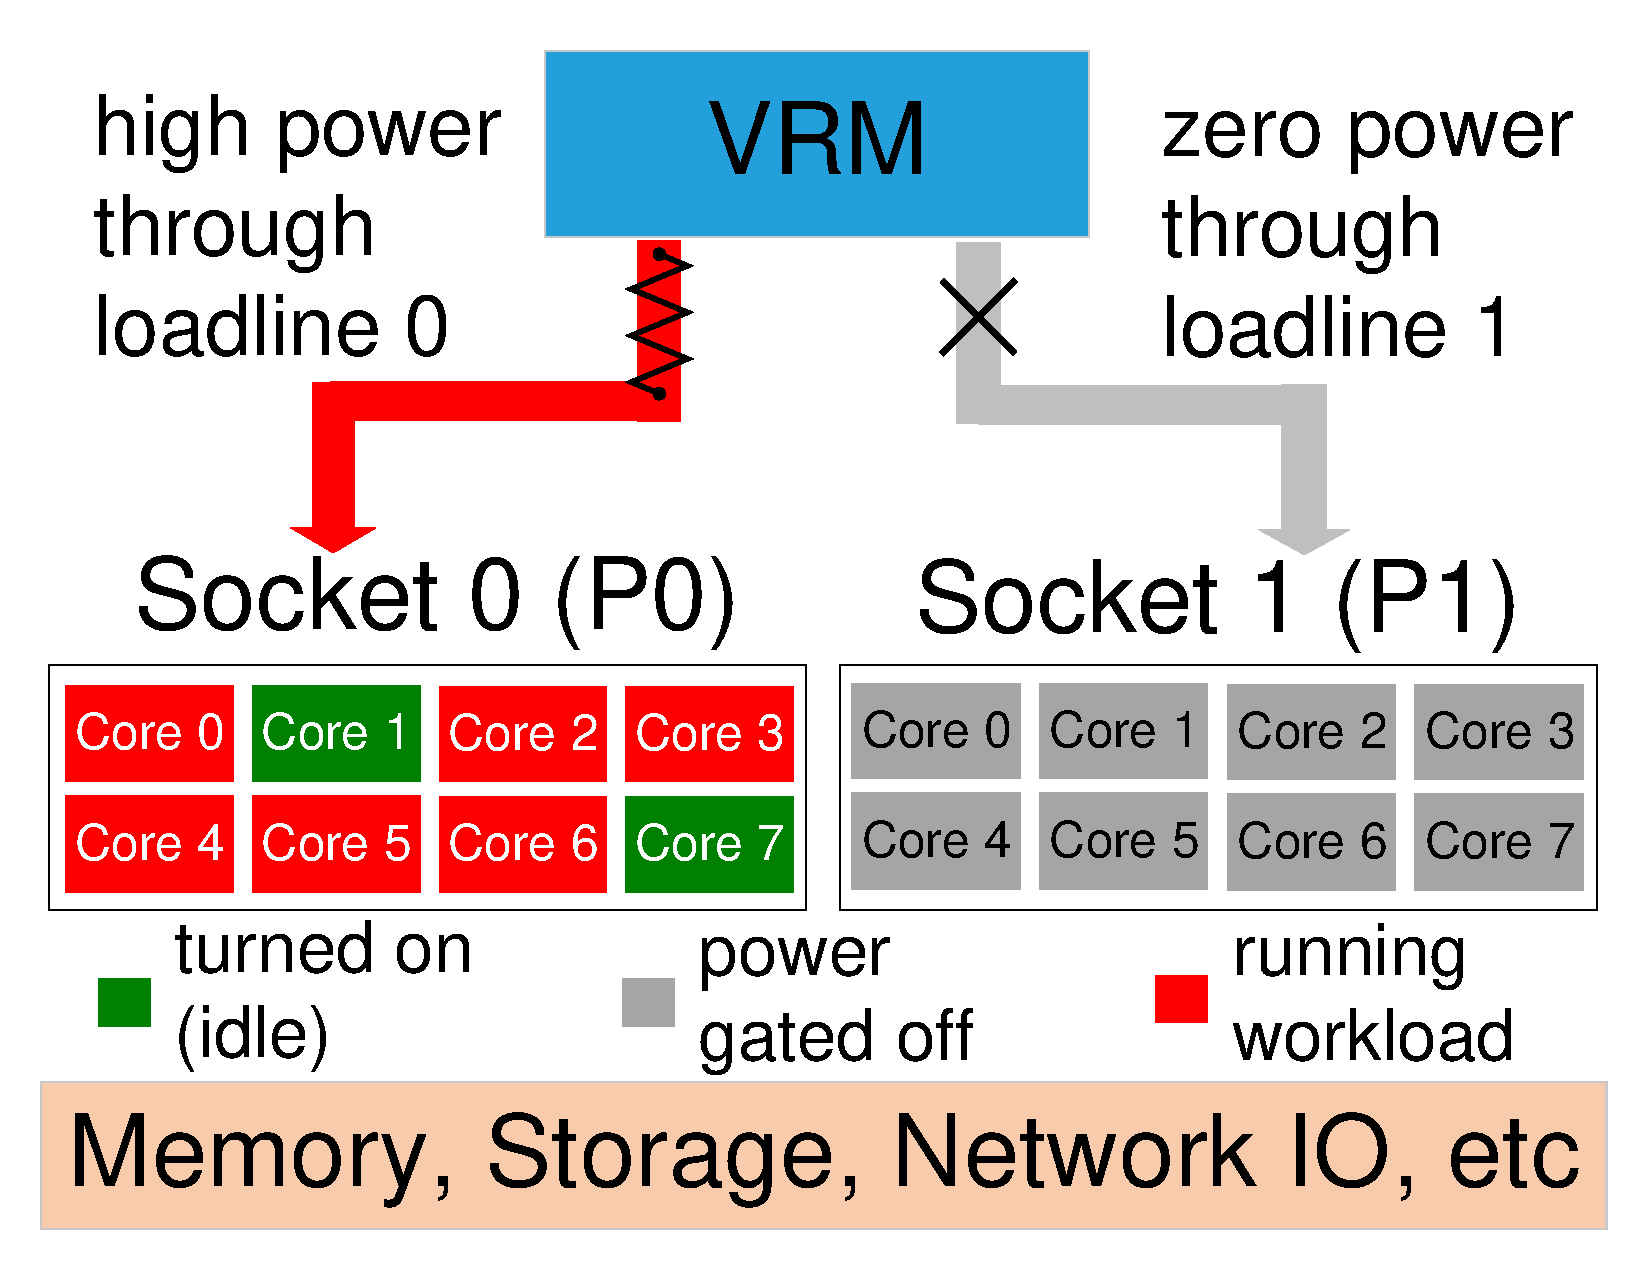
\includegraphics[trim=0 0 0 0,clip,width=.43\linewidth]{graphs/voltage/loadline-borrowing_diagram1.pdf}
    \label{fig:ll-borrow-idea1} 
}
\hfill
\subfloat[Loadline borrowing.] {
    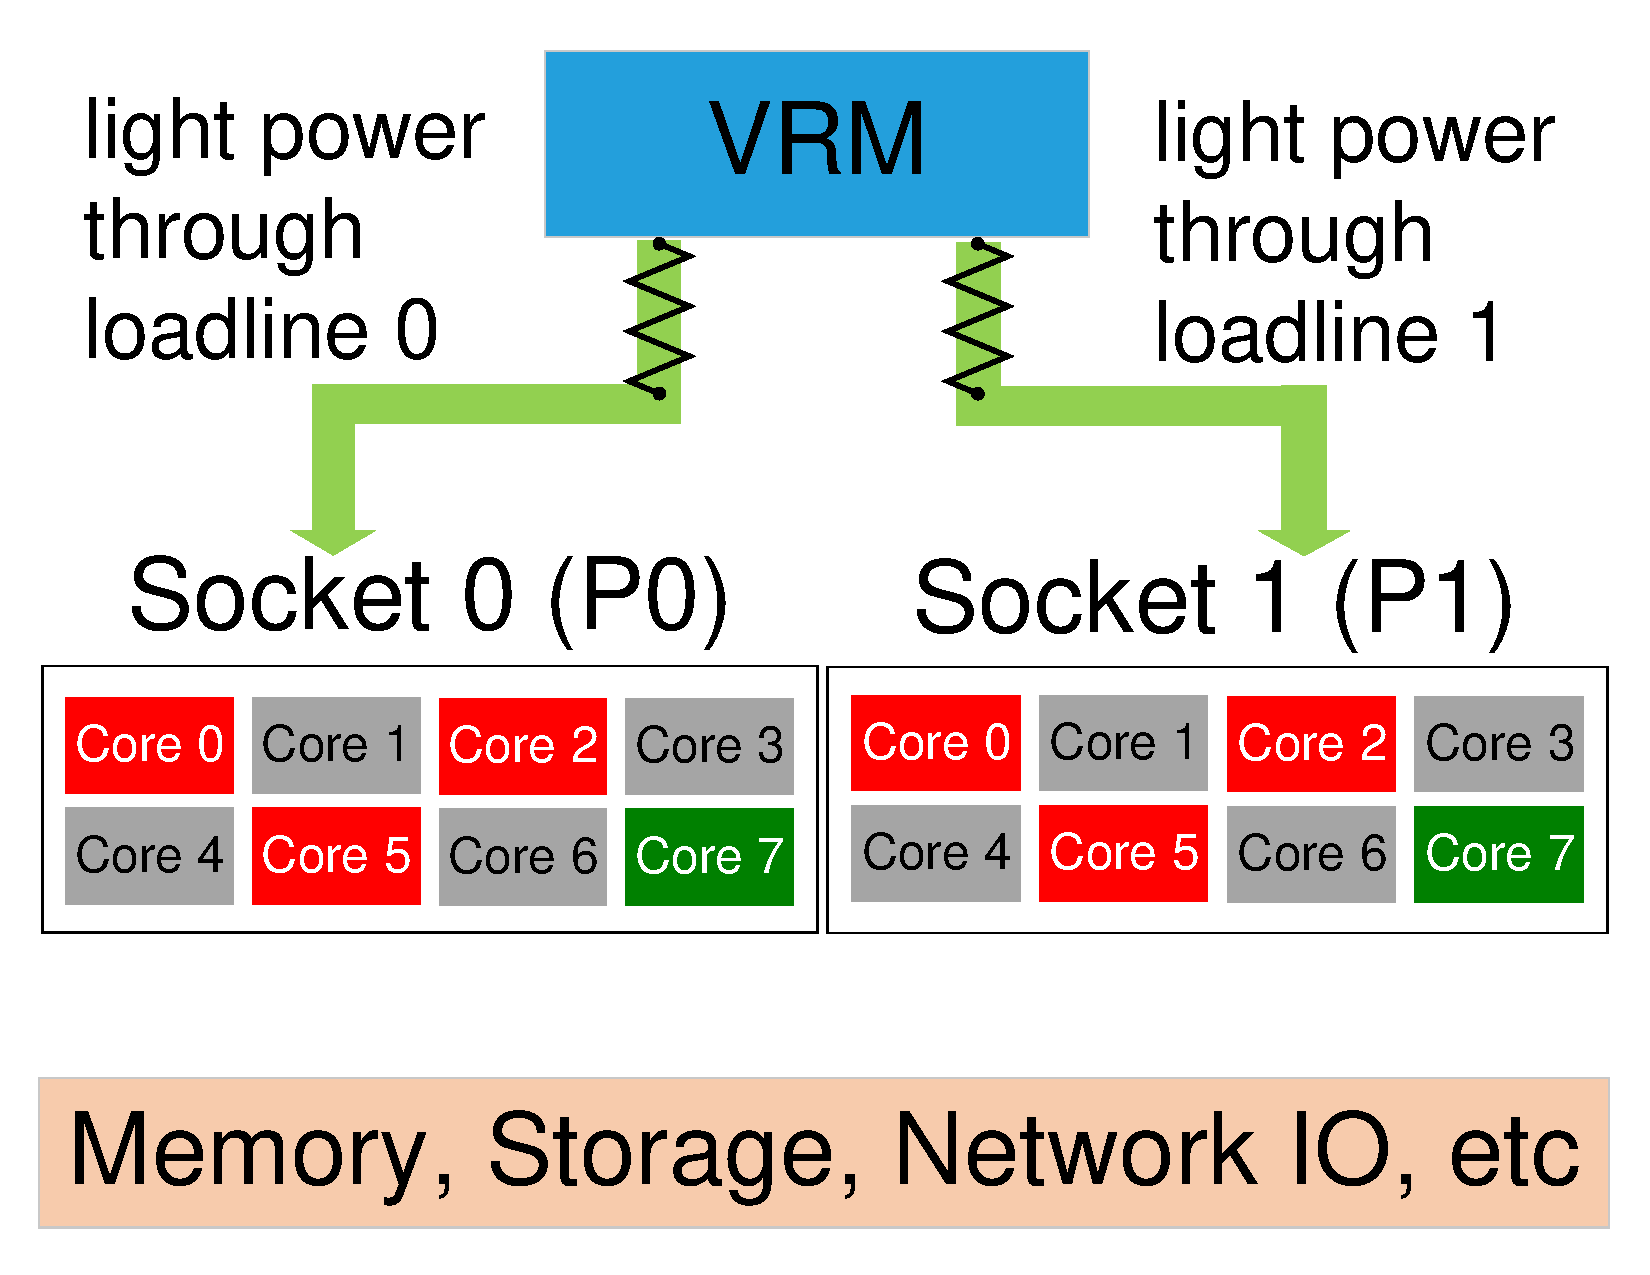
\includegraphics[trim=0 0 0 0,clip,width=.43\linewidth]{graphs/voltage/loadline-borrowing_diagram2.pdf}
    \label{fig:ll-borrow-idea2} 
}
\caption{Loadline borrowing balances workloads across multiple sockets to reduce per-socket voltage drop and create room for active timing margin.}
%\vspace*{-0.4cm}
\label{fig:ll-borrow-idea}
\end{figure}

\subsection{Solution for Recovering Multicore Scaling Loss}
\label{sec:voltage:opt:loadline}

We use~\Fig{fig:ll-borrow-idea} to introduce how loadline borrowing optimizes workload distribution among a server's VRM-multiprocessor subsystem. In~\Fig{fig:ll-borrow-idea}, multiple processor sockets share a common VRM chip, each with its own power delivery path from the VRM to the die. The VRM can generate multiple V$_{dd}$ levels for different processors, which is normal for contemporary systems. In the following discussion, we use~\Fig{fig:ll-borrow-idea1} and \Fig{fig:ll-borrow-idea2} to analyze the scenarios of workload consolidation and loadline borrowing and highlight the necessity of considering VRM's role in systems with active timing margin processors. Other components such as memory chips and disks are powered on steadily throughout our analysis.

\Fig{fig:ll-borrow-idea1} shows a traditional consolidation schedule for a multisocket server. Workloads are all mapped to socket 0 so that socket 1 can be shut down. Because all power goes to socket 0, the passive voltage drop along the power-delivery path from VRM to processor 0 is very high, which limits active timing margin's potential to undervolt.

Loadline borrowing balances workloads equally among all available sockets, and power gates off unneeded cores to eliminate idle power consumption.~\Fig{fig:ll-borrow-idea2} illustrates a loadline-borrowing schedule. In~\Fig{fig:ll-borrow-idea2} active cores are distributed to each socket evenly, and each socket power gates off a set of unused cores to achieve the same idle power elimination effect as in a consolidated schedule. In this schedule, each socket draws less power, reducing the passive voltage drop each processor experiences. This allows active timing margin to reduce more voltage from each processor and hence improve total processor power.

We use our two-socket platform to illustrate the benefits of loadline borrowing. We compare the case of conventional workload consolidation, which places all loaded cores on one processor as the baseline, to loadline borrowing, which balances the loaded core count across both processors. We keep eight of the total 16 cores turned on to respond instantly to utilization levels of up to 50\%. The remaining eight cores are assumed to be not instantly needed, and therefore are put into a deep sleep (power-gated) state. We run the workload using one to eight cores. In the conventional case, all of the turned-on cores reside on a single processor. In the loadline borrowing case, each processor has four cores that are turned on and active. In either case, we measure and compare the two processors' total chip power.

\begin{figure}[t]
\centering
\vspace*{-10pt}
\subfloat[Undervolt scaling.] {
    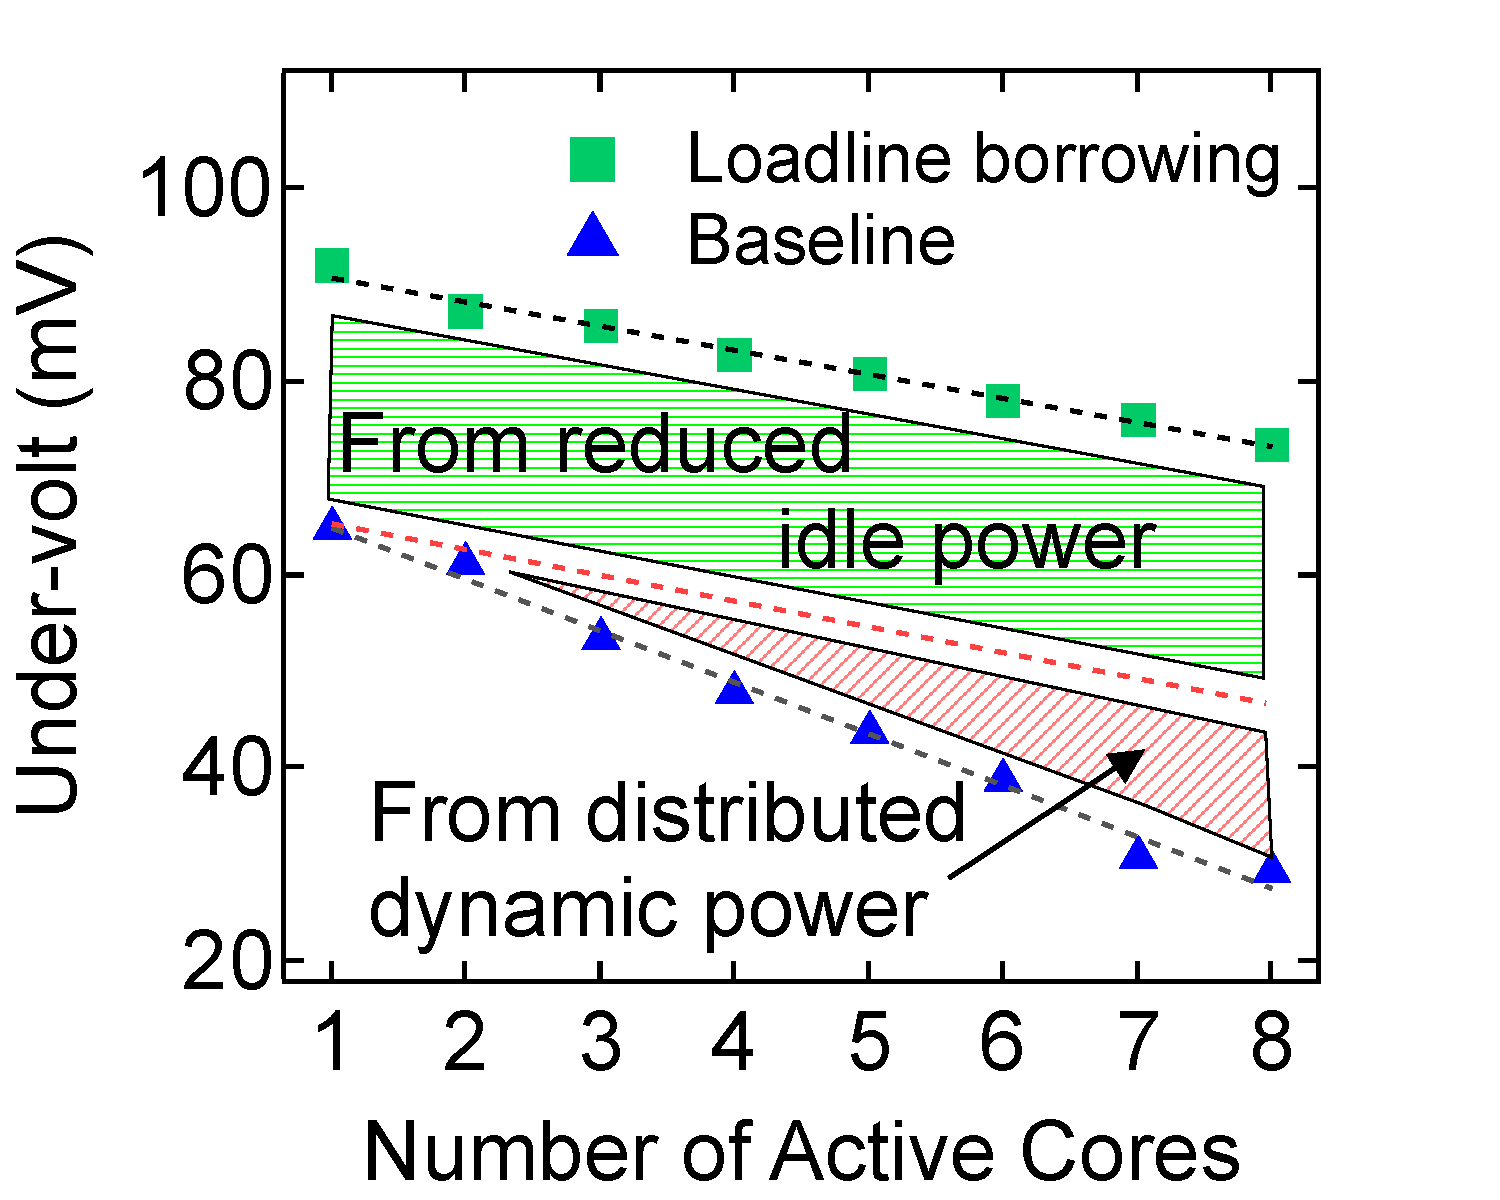
\includegraphics[trim=0 0 65 0,clip,width=.43\linewidth]{graphs/voltage/raytrace_split_uv.pdf}
    \label{fig:split_raytrace_uv} 
}
\hfill
\subfloat[Power scaling.] {
    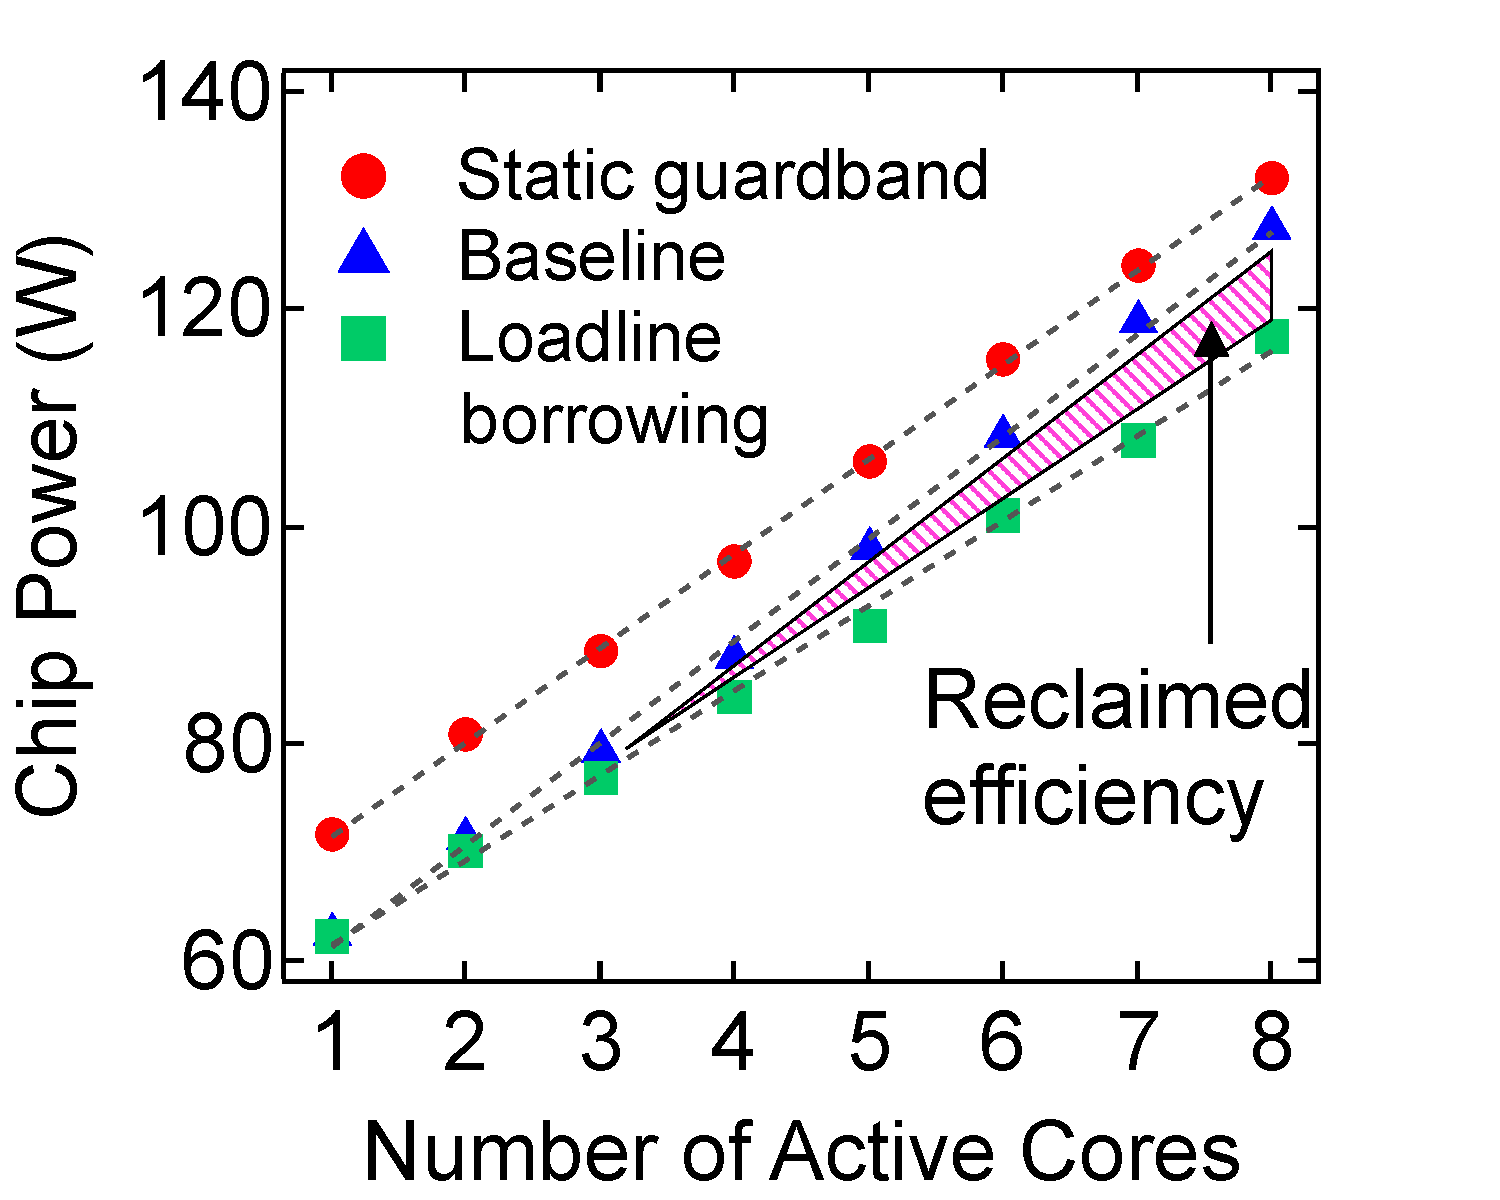
\includegraphics[trim=0 0 65 0,clip,width=.43\linewidth]{graphs/voltage/raytrace_split_pwr.pdf}
    \label{fig:split_raytrace_pwr} 
}
\caption{Distributing \benchmark{raytrace} across two processors reduces passive voltage drop, allowing more power saving under high core count.}
\vspace{-0.4cm}
\label{fig:split_raytrace}
\end{figure}

As an example, \Fig{fig:split_raytrace} shows the results for \benchmark{raytrace} with loadline borrowing. \Fig{fig:split_raytrace_uv} shows that loadline borrowing offers a better undervolting benefit no matter how many cores are used. There are two reasons. First, loadline borrowing lets each processor power on fewer cores, which cuts down leakage power, and thus substantially reduces the idle power. For~\benchmark{raytrace}, less idle power gives 20mV more undervolting benefit when one core is active. Second, balancing application activity (threads) and system requirements (idle cores) across the processors' loadline distributes dynamic power across each processor, which further reduces the passive drop for each processor. When eight cores are active, reduced dynamic power allows an additional 20mV reduction. 

\Fig{fig:split_raytrace_pwr} shows loadline borrowing can reduce a significant amount of total chip V$_{dd}$ power. The biggest effect is achieved when more cores are used. In~\Fig{fig:split_raytrace_pwr} loadline borrowing reduces power consumption by 1.6\%, 4.2\% and 8.5\% when two, four and eight cores are used, respectively. The result is intuitive because each processor's passive voltage drop is reduced when fewer cores are active. Thus, distributing the workload when more cores are active yields larger benefits. 

Loadline-borrowing is suitable only for workload scheduling within a multisocket server. In this setting, all other resources, such as memory, disk and network I/O, remain active when workloads are consolidated onto a few processors. When workloads are consolidated across multiple servers, the idle power reduction from turning off the used memory and hard drive outweighs active timing margin's processor power savings. In this case, the scheduler will consolidate workloads onto fewer servers first, then on each server loadline borrowing can be used to further improve cluster power consumption. We leave this discussion to future studies.

\subsection{Power Reduction Improvement}
\label{sec:voltage:opt:result}

\begin{figure}[t]
\centering
    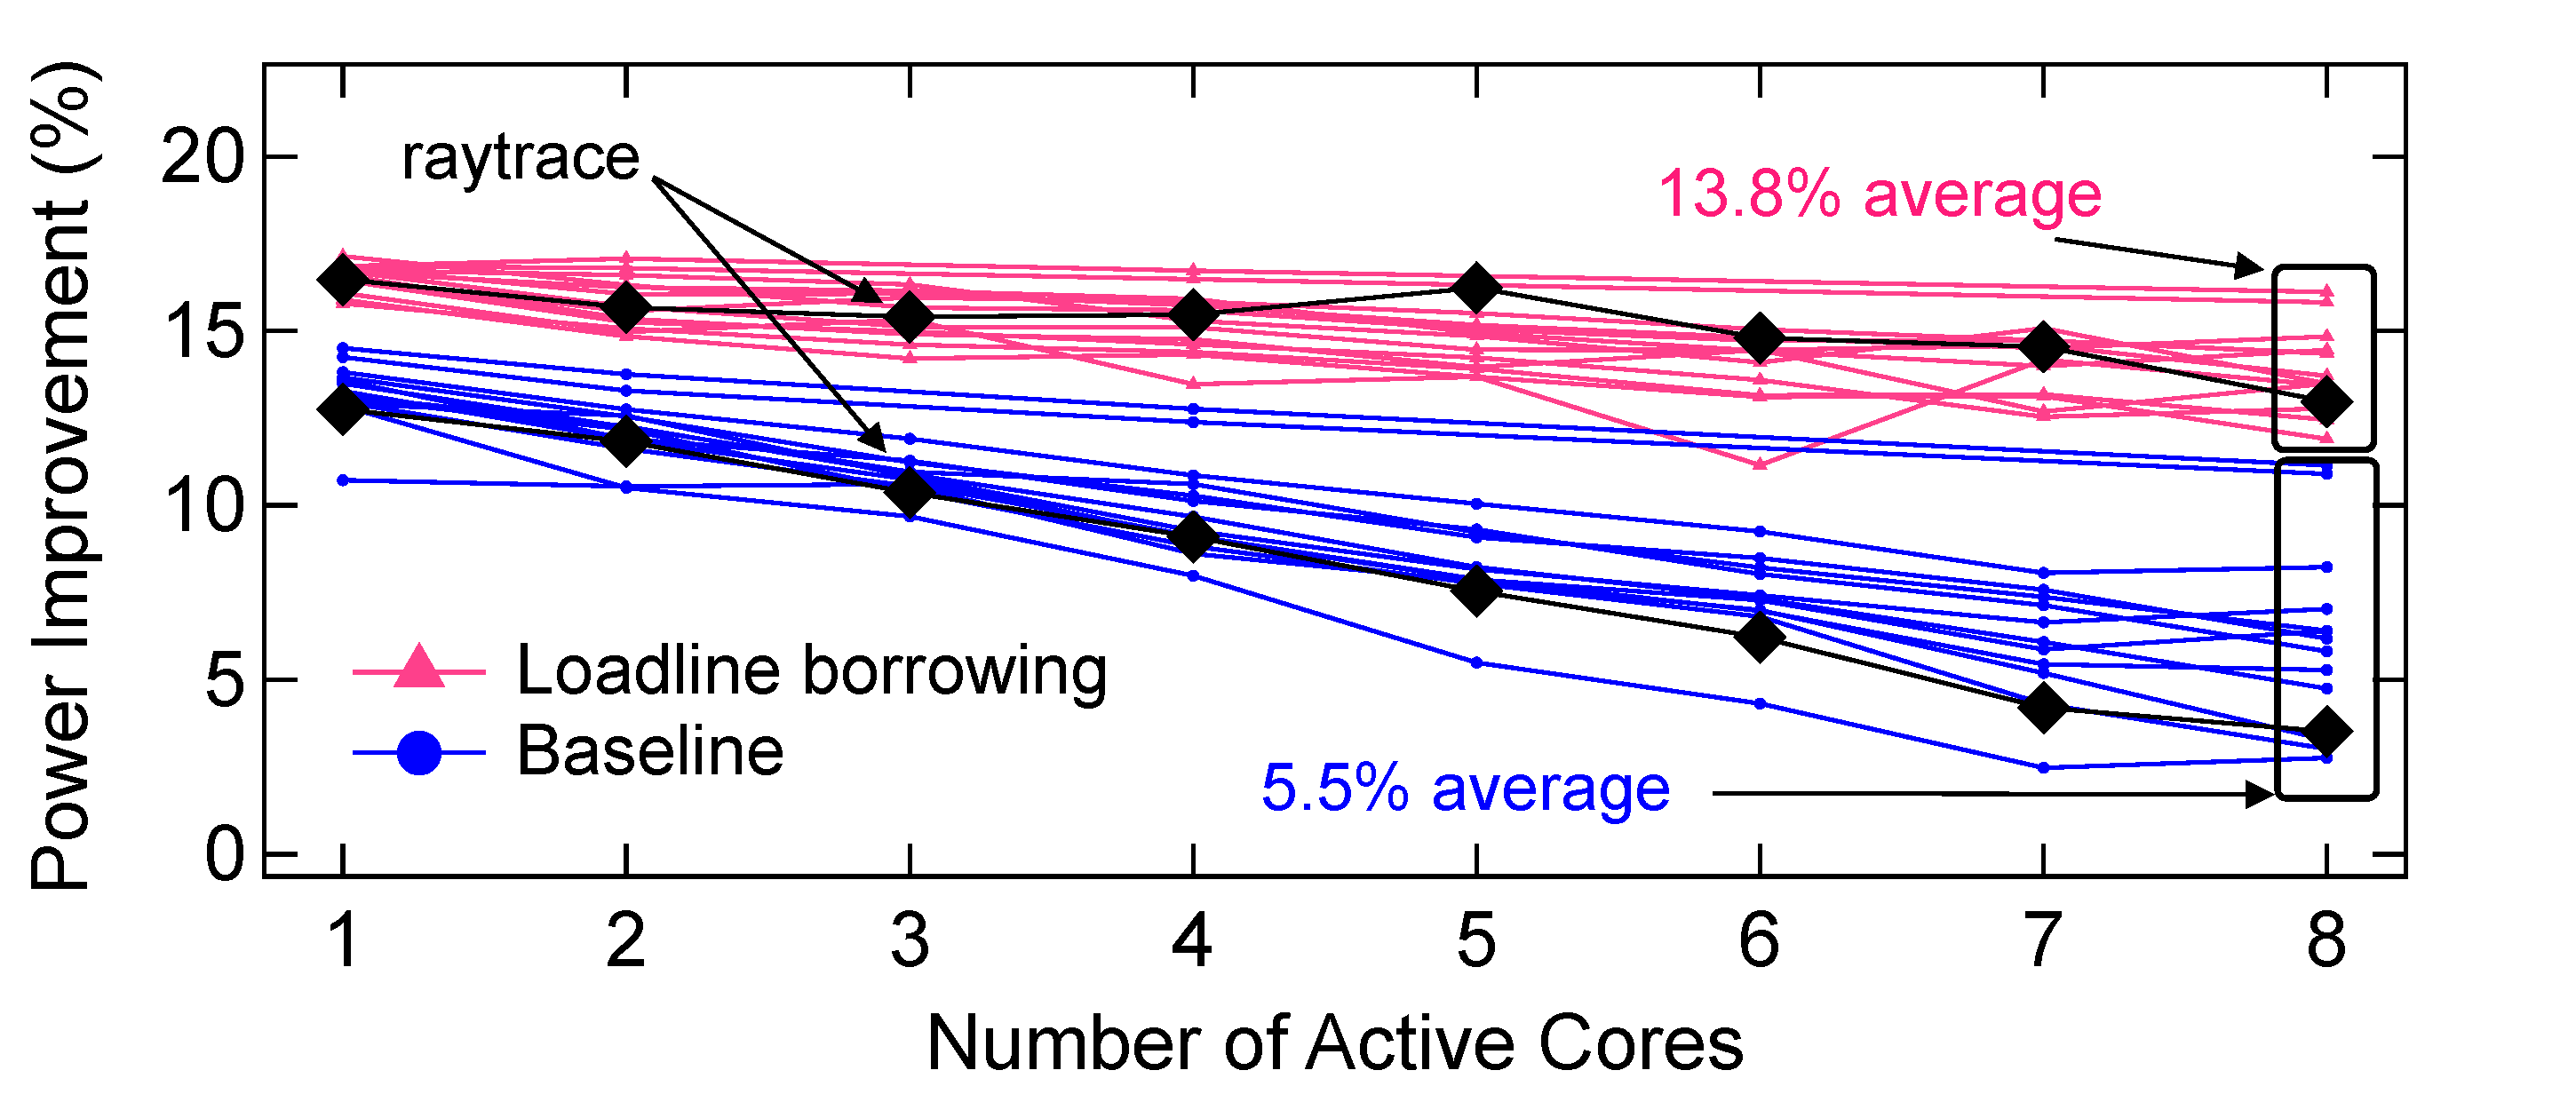
\includegraphics[trim=0 0 0 0, clip,width=0.8\linewidth]{graphs/voltage/loadline-borrowing_scale.pdf}
    \caption{Loadline borrowing's power and energy improvement under different numbers of active cores. Compared to the baseline, loadline borrowing consistently shifts up every workload's power improvement.}
    \label{fig:ll-borrow-scale}
    \vspace{-0.2cm}
\end{figure}

\begin{figure*}[t]
\centering
    \vspace{0.4in}
    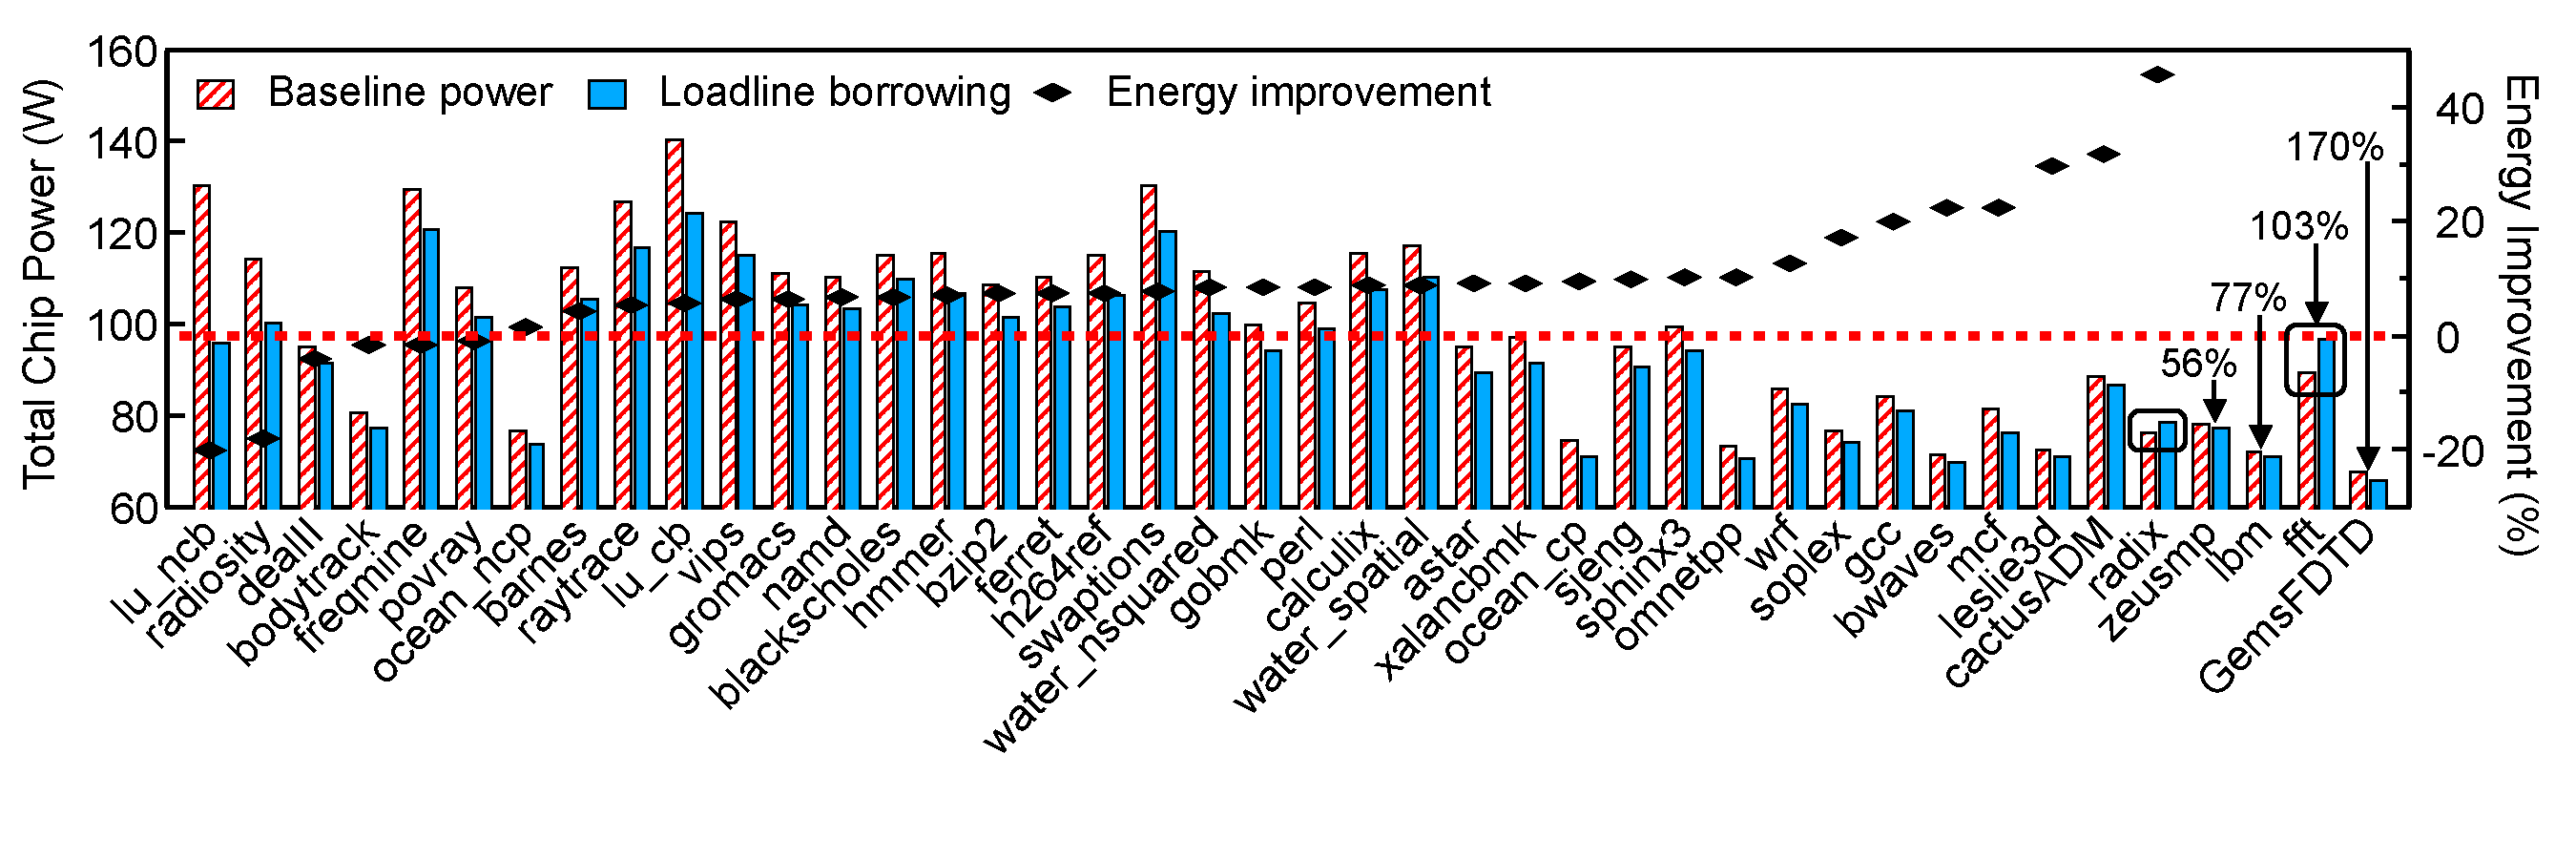
\includegraphics[trim=0 0 0 0,clip,width=\linewidth]{graphs/voltage/split_benefits_all.pdf}
    \caption{Loadline borrowing's power and energy improvement when eight cores are active.}
    \label{fig:ll-borrow-8core-normal}
\end{figure*}

Current operating systems are unaware and do not incorporate loadline knowledge into process scheduling. We use the Linux kernel's taskset affinity mechanism to emulate a schedule that dynamically performs loadline borrowing. We evaluate loadline borrowing on a wider set of benchmarks including all of PARSEC and SPLASH-2 workloads to capture the general trends. Briefly, the key highlight is that loadline-aware OS-level software scheduling can effectively \emph{double the efficiency} of active timing margin at high core counts.

\Fig{fig:ll-borrow-scale} shows active timing margin's scaling power improvement against static guardbanding under workload consolidation and loadline borrowing. Ideally, active timing margin's power improvement will not scale down, and it will be identical across workloads. Loadline borrowing approaches this goal by increasing active timing margin's power-saving capability for all active cores, shown by the clustered lines at the top of the figure. When fewer cores are active, loadline borrowing's power improvement comes mainly from the reduced idle power on each processor. The improvement increases when more cores are active because each chip's dynamic power also reduces when the workload is distributed. \Fig{fig:ll-borrow-scale} shows that on average consolidated active timing margin achieves 5.5\% power improvement over static guardbanding when eight cores are active, whereas loadline borrowing improves by 13.8\%, over 50\% improvement atop the original system design.

We study more benchmarks along with PARSEC and SPLASH-2, including SPEC CPU 2006 workloads running in the form of SPECrate~\cite{SPECrate}, to further demonstrate loadline borrowing's power and energy improvement when all eight cores are active. SPECrate is commonly used to measure system throughput, typical of evaluating performance when running different tasks simultaneously. We use 32 PARSEC and SPLASH-2 threads and eight SPECrate workload copies to match POWER7+'s eight-core architecture. The results are shown in \Fig{fig:ll-borrow-8core-normal}. On average, loadline borrowing achieves 6.2\% and 7.7\% reduction in power and energy, respectively, across the workloads. For power-intensive workloads such as \benchmark{lu\_cb}, loadline borrowing can achieve 12.7\% power improvement. 

A handful of benchmarks fall into one of two extremes. On one extreme, some benchmarks that are to the leftmost side on the $x$-axis, such as \benchmark{lu\_ncb} (not to be confused with \benchmark{lu\_cb}) and \benchmark{radiosity}, suffer from severe performance loss. Performance decreases by more than 20\% due to interchip communication overhead (not shown). This in part leads to reduced core power consumption during loadline borrowing (see left $y$-axis), but the longer execution time negatively offsets the benefit and increases total energy consumption. 

On the other extreme, some other benchmarks that are to the rightmost side on the $x$-axis, such as \benchmark{radix}, \benchmark{zeusmp}, \benchmark{lbm}, \benchmark{fft} and \benchmark{GemsFDTD}, experience large performance improvements from load balancing because there is less memory subsystem contention. This performance improvement increases chip activity that could sometimes lead to higher power consumption than the baseline system, such as in the case of \benchmark{radix} and \benchmark{fft}. Nonetheless, the improved performance brings about large energy reductions for these workloads, as the right \textit{y}-axis in~\Fig{fig:ll-borrow-8core-normal} shows. Improvements range between 50\% and 171\%.

\subsection{Related Work}
\label{sec:voltage:related}

The $di/dt$ effect and its impact on reliability has been well noted~\cite{james2007comparison,reddi2010voltage,kim2012audit,bertran2014voltage}. A plethora of work aims at reducing inductive noise in microprocessors, ranging from the circuit~\cite{ernst2003razor,blaauw2008razorii}, architecture~\cite{grochowski2002microarchitectural,powell2003pipeline,gupta2007understanding,gupta2008decor,gupta2009event,reddi2009voltage,reddi2010voltage,miller2012vrsync,zhang2014architecture} and software~\cite{reddi2010eliminating}. These works usually require intrusive design changes to the hardware~\cite{ernst2003razor,blaauw2008razorii,gupta2008decor,reddi2009voltage} and rely on simulation, microarchitecture event detection and activity throttling~\cite{grochowski2002microarchitectural,powell2003pipeline,gupta2009event,reddi2009voltage,reddi2010eliminating,miller2012vrsync}.

Unlike the prior work, we use a measurement-based approach to studying adaptive guardbanding processors~\cite{fischer200590nm,tschanz2007adaptive,kurd2008next,lefurgy2011active,bowman201222nm} that handles droops in a fundamentally new way. Because adaptive guardbanding can effectively improve efficiency and guarantee reliability at the same time, it has gained more attention recently~\cite{grenat20145,tokunaga20145,bowman20158}.

Prior work on adaptive guardbanding focuses on voltage droop tolerance and system-efficiency analysis at one core or one processor level ~\cite{fischer200590nm,tschanz2007adaptive,kurd2008next,lefurgy2011active,bowman201222nm,grenat20145,tokunaga20145,bowman20158}. In our work, we showcase adaptive guardbanding's system-level implications for core scaling and workload heterogeneity, and we investigate its root causes. Our analysis incorporates $di/dt$ noise and extends to total on-chip voltage drop. Our multicore $di/dt$ noise characterization confirms prior observations~\cite{gupta2007understanding,reddi2010voltage,miller2012vrsync}. We also observe mitigated typical-case noise and magnified worst-case noise~\cite{miller2012vrsync} due to on-chip noise propagation~\cite{gupta2007understanding,reddi2010voltage}. Because adaptive guardbanding deals with $di/dt$ noise well, further investigation should focus on improving its performance with respect to passive voltage drop.